\documentclass[a4paper,10pt]{article}
\usepackage[utf8]{inputenc}

% ----  Useful packages % ---- 
\usepackage{amsmath}
\usepackage{graphicx}
\usepackage{amsfonts} 
\usepackage{amsthm}
\usepackage{amssymb}
\usepackage{makecell}
\usepackage{tikz}
\usetikzlibrary{arrows.meta}
% ----  Useful packages % ---- 

\usepackage{pythonhighlight}
\usepackage{wrapfig}
\usepackage{caption}
\usepackage{subcaption}
\usepackage{hyperref}
\hypersetup{
	colorlinks,
	citecolor=black,
	filecolor=black,
	linkcolor=black,
	urlcolor=black
}

% ---- Set page size and margins replace ------
\usepackage[letterpaper,top=2cm,bottom=2cm,left=3cm,right=3cm,marginparwidth=1.75cm]{geometry}
% ---- Set page size and margins replace ------

% ------- NOTA ------
\theoremstyle{remark}
\newtheorem{note}{Note}[subsection]
% ------- NOTA ------

% ------- OSSERVAZIONE ------
\theoremstyle{definition}
\newtheorem{observation}{Osservazione}[subsection]
% ------- OSSERVAZIONE ------

% ------- DEFINIZIONE ------
\theoremstyle{plain}
\newtheorem{definition}{Definizione}[subsection]
% ------- DEFINIZIONE ------

% ------- ESEMPIO ------
\theoremstyle{definition}
\newtheorem{example}{Esempio}[subsection]
% ------- ESEMPIO ------

% ------- DIMOSTRAZIONE ------
\theoremstyle{definition}
\newtheorem{demostration}{Dimotrazione}[subsection]
% ------- DIMOSTRAZIONE ------

% ------- TEOREMA ------
\theoremstyle{definition}
\newtheorem{theorem}{Teorema}[subsection]
% ------- TEOREMA ------

% ------- COROLLARIO ------
\theoremstyle{plain}
\newtheorem{corollaries}{Corollario}[theorem]
% ------- COROLLARIO ------

% ------- PROPOSIZIONE ------
\theoremstyle{plain}
\newtheorem{proposition}{Proposizione}[subsection]
% ------- PROPOSIZIONE ------

% ---- Footer and header ---- 
\usepackage{fancyhdr}
\pagestyle{fancy}
\fancyhf{}
\fancyhead[LE,RO]{A.A 2023-2024}
\fancyhead[RE,LO]{Introduzione all'intelligenza artificiale}
\fancyfoot[RE,LO]{\rightmark}
\fancyfoot[LE,RO]{\thepage}

\renewcommand{\headrulewidth}{.5pt}
\renewcommand{\footrulewidth}{.5pt}
% ---- Footer and header ---- 

% ----  Language setting ---- 
\usepackage[italian, english]{babel}
% ----  Language setting ---- 

\usepackage{listings}
\usepackage{color}

\definecolor{dkgreen}{rgb}{0,0.6,0}
\definecolor{gray}{rgb}{0.5,0.5,0.5}
\definecolor{mauve}{rgb}{0.58,0,0.82}

\lstset{frame=tb,
	language=C,
	aboveskip=3mm,
	belowskip=3mm,
	showstringspaces=false,
	columns=flexible,
	basicstyle={\small\ttfamily},
	numbers=none,
	numberstyle=\tiny\color{gray},
	keywordstyle=\color{blue},
	commentstyle=\color{dkgreen},
	stringstyle=\color{mauve},
	breaklines=true,
	breakatwhitespace=true,
	tabsize=3
}

\title{\textbf{Introduzione all'Intelligenza Artificiale}}
\author{Realizzato da: Matteo Giuntoni, Ghirardini Filippo}
\date{A.A. 2023-2024}

\begin{document}
	\begin{titlepage} %crea l'enviroment
	\begin{figure}[t] %inserisce le figure
		\centering
\includegraphics[width=0.98\textwidth]{marchio_unipi_pant541.png}
	\end{figure}
	\vspace{20mm}
	
	\begin{Large}
		\begin{center}
			\textbf{Dipartimento di Informatica\\ Corso di Laurea Triennale in Informatica\\}
			\vspace{20mm}
			{\LARGE{Corso a Libera Scelta - 6 CFU}}\\
			\vspace{10mm}
			{\huge{\bf Computer Graphics}}\\
		\end{center}
	\end{Large}
	
	
	\vspace{36mm}
	%minipage divide la pagina in due sezioni settabili
	\begin{minipage}[t]{0.47\textwidth}
		{\large{\bf Professore:}\\ \large{Prof. }}
	\end{minipage}
	\hfill
	\begin{minipage}[t]{0.47\textwidth}\raggedleft
		{\large{\bf Autore:}\\ \large{Filippo Ghirardini}}
	\end{minipage}
	
	\vspace{25mm}
	
	\hrulefill
	
	\vspace{5mm}
	
	\centering{\large{\bf Anno Accademico 2023/2024 }}
	
\end{titlepage}
	
	\tableofcontents
	\newpage
	\maketitle
	\begin{center}
		\vspace{-20pt}
		\rule{11cm}{.1pt} 
	\end{center}
	\section{Punto materiale}
Oggetto caratterizzato da una massa [kg] e da un vettore posizione [m] nello spazio 3D.
Dimensioni trascurabili, forma irrilevante rispetto ai fenomeni di interesse.
Vettore posizione come funzione del tempo t[s].
\begin{example}
    Una molecola di ossigeno se sono interessato all'aereodinamica di una vettua. 
    Un satellite attorno alla terra se ignoro le forze di marea.
\end{example}
\hspace{-15pt}\textbf{Un vettore posizione} è una funzione del tempo $t[s]$.
$$\vec{r(t)} = (x(t), y(t), z(t)) = x(t)\hat{x} + y(t)\hat{z} + z(t)\hat{z}$$
\begin{observation}
    I versori cartesiani sono costanti
\end{observation}

\begin{definition}[Legge oraria]
    Si definisce come legge oraria la funzione $t \mapsto \vec{r}(t)$.
\end{definition}

\begin{definition}[Traiettoria]
    Il luogo geometrico di punti visitati dal punto materiale.
    $$\{\vec{r}(t)\:\: per \: t \in \mathbb{R}\}$$
\end{definition}

\begin{example}
    $\vec{r}(t) = (v_0t, y_0, 0)$ e $v_0 = 3m/s, y_o = 5m$ 
    \begin{figure}[h!]
        \centering
        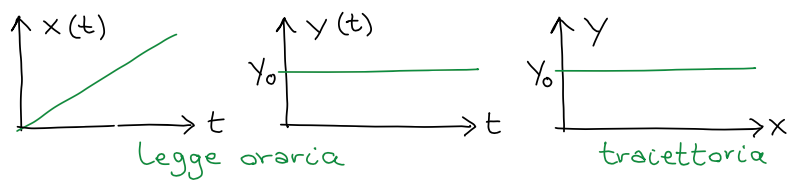
\includegraphics[width=0.8\textwidth]{images/ess-traiettoria.png}
    \end{figure}
\end{example}

\begin{definition}
    La \textbf{velocità istantanea} è la derivata della posizione rispetto al tempo.
    $$v = \lim_{\Delta t \to 0}\frac{\Delta s}{\Delta t} = \frac{ds}{dt}$$
\end{definition}

\begin{definition}
    La \textbf{velocità media} è definita come il rapporto tra lo spostamento e l'intervallo di tempo necessario per effettuarlo.
    $$v_m = \frac{\Delta s}{\Delta t}$$
\end{definition}
\hspace{-15pt}In parole povere è una grandezza che ci dice con quale rapidità cambia la posizione di un punto rispetto al tempo nell'instante $t$.
\subsection*{Vettore velocità}
Derivata rispetto al tempo del vettore posizione e si indica come 
$\frac{d\vec{r}(t)}{dt}\text{ oppure }\dot{\vec{r}}(t)[m/s]$
\begin{equation}
    \begin{split}
    \dot{\vec{r}}(t) & = (\dot{x}(t), \dot{y}(t), \dot{z}(t)) \\
     & = \frac{d}{dt}[x(t)\hat{x} + y(t)\hat{y} + z(t)\hat{z}] \\
     & = \dot{x}(t)\hat{x} + \dot{y}(t)\hat{y} + \dot{z}(t)\hat{z}
    \end{split}
\end{equation}
Per ricavare la forma esplicita uso le proprietà delle derivate (\textbf{linearità}, \textbf{Leibnitz})
\begin{example}
    $\vec{r}(t) = (v_0t, y_0, 0) = v_0t\hat{x} + y_0\hat{y}$ \:\:\:abbiamo che \:\:\:
    $\dot{\vec{r}}(t) = (v_0, 0, 0) = v_0 \hat{x}$
\end{example}
\hspace{-15pt}Velocità e spazio percorso ("integrale di linea").\\
\begin{wrapfigure}[3]{l}{5cm}
    \centering
    \includegraphics[width=5cm]{images/vettore-velocità.png}
\end{wrapfigure}
\begin{align*}
    L & = ||\vec{r}(t_1) - \vec{r}(t_0)|| + ||\vec{r}(t_2) - \vec{r}(t_1)|| + ||\vec{r}(t_3) - \vec{r}(t_2)|| + \dots \\
    & = \sum_i ||\vec{r}(t_{i+1} - \vec{r}(t_i)|| \:\: per\:\: |t_{i+1} - t_i| \text{"piccolo"} \\
    & = \sum_i ||\frac{\vec{r}(t_{i+1}) - \vec{r}(t_i)}{t_{i+1} - t_i}|| (t_{i+1} - t_i) = \int_{t_{in}}^{t_{f_{in}}}||\dot{\vec{r}}(t)||\\
\end{align*}
\begin{example}
    $\vec{r}(t) = (v_0t, y_0)\:\:\: \dot{\vec{r}}(t) = (v_0, 0)$\hspace{15pt}
    $||\dot{\vec{r}}(t)|| = \sqrt{v_0^2 + 0^2} = |v_0|$ \:\:\: $L = |v_0| \cdot (t_{f_{in}} - t_{in})$\\
    Il vettore è costante quindi facendo la derivata torna zero. Con la velocità si calcolo lo spazio percorso ("integrale di linea").
    La differenza fra le posizioni e la differenza dei tempi è il rapporto incrementale in caso gli intervalli siano sufficentemente
    piccoli, da qui si ottiene l'integrale.
\end{example}

\subsection{Vettore accelerazione}
Derivata rispetto al tempo del vettore velocità e si indica con $\frac{d^2\vec{r}(t)}{dt} \text{ oppure } \ddot{\vec{r}}(t) [m/s^2]$
\begin{equation}
    \ddot{\vec{r}}(t) = (\ddot{x}(t), \ddot{y}(t), \ddot{z}(t))\:\: = \:\: \ddot{x}(t)\hat{x} + \ddot{y}(t)\hat{y} + \ddot{z}(t)\hat{z}
\end{equation}
\begin{example}
    $\vec{r}(t)= (\frac{1}{2}a_0t^2, v_0t, 0)$ \hspace{10pt} $\dot{\vec{r}}(t) = (a_0t, v_0, 0)$ \hspace{10pt} $\dot{\vec{r}}(t) = (a_0, 0, 0)$
\end{example}
\hspace{-15pt}Serve perché l'equazione "del moto" di Newton che determinata la legge oraria è formulata in termini di accelerazione.

\subsection{Vettore quantità di moto}
Il prodotto di massa [kg] e velocità [m/s]
$$\vec{p}(t) = m \cdot \dot{\vec{r}}(t) = (m\dot{x}(t), m\dot{y}(t), m\dot{x}(t)) = m\dot{\vec{x}}(t)x + m\dot{\vec{y}}(t)y + m \dot{\vec{z}}(t)z$$
\begin{example}
    Prendiamo un punto di massa 2kg e velocità 3m/s lungo $\hat{x}$.\\
    $p_x(t) = 2 \cdot 3 kg\cdot m/s = 6 kg \cdot m/s$ \hspace{15pt} $p_y(t) = p_z(t) = 0$.
\end{example}
\hspace{-15pt}Serve per generalizzare l'equazione di Newton e per trattare sistemi di piu punti materiali.

\subsection{Vettore momento angolare rispetto a un polo P}
$$\vec{L}_p(t) = m(\vec{r}(t) - \vec{r}_p) \times \dot{\vec{r}}(t)$$
Dove $\vec{r}_p$ è il vettore posizione di p, mentre $\dot{\vec{r}}(t)$ è il prodotto vettoriale.
\begin{example}
    $\vec{r}_p = (l_0, 0, 0)$ \hspace{15pt} $\vec{r}(t) = (v_0t, y_0, 0)$\\
    $\vec{L}_p = m[(v_0t - l_0)\hat{x} + y_0\hat{y}] \times (v_0\hat{x}) \:\: = \:\: m(v_0t - l_0)v_0 \hat{x} \times \hat{x} + my_0v_0\hat{y}\times \hat{x} 
    \:\: = \:\: my_0v_0(-\hat{z}) = (0,0, -my_0v_0)$\\
    Ricorda che $\hat{x} \times \hat{x} = 0$ e $\hat{y} \times \hat{x} = -\hat{z}$
\end{example}
\hspace{-15pt}Il momento angolare dice quanta inerzia ha un oggetto in una rotazione (descrizione sommaria).\\
Il polo P è parte della definizione. È una scelta! Il risultato dipende dal polo.
Serve per formulare l'equazione del moto di sistemi di punti materiali e corpi rigidi.

\subsection{Coordinate polari}
Un metodo per rapprensentare delle cordinate x, y andando a misurare prima la distanza dall'origine e poi si va a vedere
quanto vale l'angolo fra questo segmento dall'asse x, utilizzando seno e coseno.
\begin{wrapfigure}[7]{l}{2cm}
    \centering
    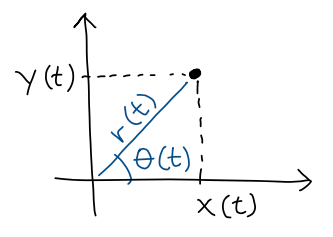
\includegraphics[width=5.5cm]{images/coordinate-polari.png}
\end{wrapfigure}
\begin{align*}
    \begin{cases}
        x(t) = r(t) \cdot \cos(\Theta(t))\\
        y(t) = r(t) \cdot \sin(\Theta(t)) 
    \end{cases}
\end{align*}
\begin{align*}
    \begin{cases}
        r(t) = \sqrt{x(t)^2 + y(t)^2} \geq 0\\
        tg(\Theta(t)) = y(t) / x(t) 
    \end{cases}
\end{align*}
\\
\begin{example} Esempi di rappresentazione di coordinate in coordinate polari.\\
    $x = 0, y = l_0 > 0 \:\: \Rightarrow \:\: r = l_0, \Theta = \pi/2$\\
    $x = 0, y = -l_0 < 0 \:\: \Rightarrow \:\: r = l_0, \Theta = -\pi/2$\\
    $x = l_0, y = l_0 > 0 \:\: \Rightarrow \:\: r = \sqrt{2}l_0, \Theta = \pi/4$\\
\end{example}

\subsection{Versori polari (2D)}
Definisco un versore $\hat{r}(t)$ che punta verso il punto materiale e un versore $\hat{\Theta}(t)$ ortogonale.
Si esprime facilmente in coordinte polari.
$$\vec{r}(t) = (x(t), y(t)) = (r(t)\cos \Theta(t), r(t)\sin\Theta(t)) \:\: = \:\: r(t)(\cos\Theta(t)\hat{x} + \sin\Theta(t)\hat{y})$$
Ma $||\vec{r}(t)|| = |r(t)| = r(t)$ allora definisco $\hat{r}(t) = \vec{r}(t)/ ||\vec{r}(t)|| = \cos \Theta(t)\hat{x} + \sin\Theta(t)\hat{y}$\\\\
Trovo facilmente che un versore ortogonale è:
$$\hat{\Theta(t)} = -\sin\Theta(t)\hat{x} + \cos\Theta(t)\hat{y} \:\:\:\text{infatti} \:\:\: \hat{r}\cdot \hat{\Theta} = c \cdot (-s) + s \cdot c = 0$$
\begin{wrapfigure}[7]{r}{6cm}
    \centering
    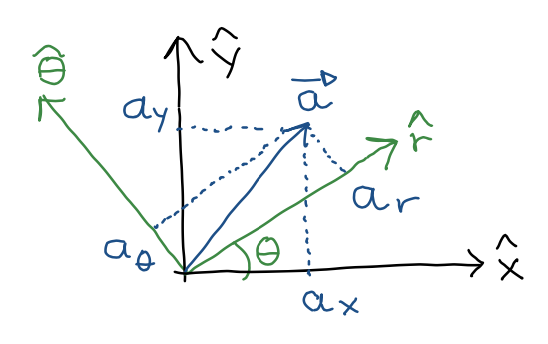
\includegraphics[width=5.5cm]{images/trasformazioni-inverse.png}
\end{wrapfigure}
\begin{note}
    Non c'è legame fra $\Theta$ e $\hat{\Theta}$ è solo una convenzione.
\end{note}
\hspace{-15pt}Le trasformazioni inverse invece si fanno come segue (verifico per sostituzione):
$$\hat{y} = \cos\Theta(t)\hat{r} - \sin\Theta(t)\hat{\Theta} \hspace{20pt} \hat{y} = \sin\Theta(t)\hat{r} + \cos\Theta(t)\hat{\Theta}$$
Possono quindi scrivere ogni vettore nella forma $\vec{a} = a_r\hat{r} + a_{\Theta}\hat{\Theta}$ con le componenti polari $a_r, a_{\Theta}$.
Per evitare ambiguità non scriviamo $(a_r, a_{\Theta})$ e riserviamo la notazione alle componenti cartesiane.\\\\
A differenza dei versori cartesiani quelli polari dipendono dal tempo per costruzioni.
$$\dot{\hat{r}}(t) = \frac{d}{dt}[\cos\Theta(t) \hat{x} + \sin\Theta(t)\hat{y}] \:\: = \:\: -\sin\Theta(t) \cdot \dot{\Theta}(t)\hat{x} + \cos\Theta(t) \cdot \dot{\Theta}(t)\hat{y}$$
Dove $\cos\Theta(t) \cdot \dot{\Theta}(t)$ si applica la derivata della somma, Leibnitz, funzione composta.
$$= \dot{\Theta}(t)\cdot \hat{\Theta}(t) \:\:\:\:(\text{confronto l'espressione di} \hat{\Theta}(t))$$
Similmente $\dot{\hat{\Theta}}(t)= - \dot{\Theta}\hat{r}(t)$.


\subsection*{Vettori posizione, velocità, accelerazione}
$$\vec{r}(t) = r(t)\hat{r}(t)$$
Dove abbiamo che $\vec{r}(t)$ è il vettore, $r(t)$ è una coordinata polare, $\hat{t}(t)$ è il versore polare.
$$\dot{\vec{r}}(r) = \dot{r}(t)\hat{r}(t) + r(t)\dot{\Theta}(t)\hat{\Theta}(t)$$
Dove la parte $\dot{\vec{r}}(r)$ è la velocità radiale.
$$\ddot{\vec{r}}(t) = [\ddot{r}(t) - r(t)\dot{\Theta}(t)^2] \hat{r} + [r(t) \ddot{\Theta}(t) + 2\dot{r}(t)\dot{\Theta}(t)]\hat{\Theta}$$
Nel quale abbiamo che la parte $r(t)\dot{\Theta}(t)^2$ si chiama \textbf{velocità centripeta}, mentre $2\dot{r}(t)\dot{\Theta}(t)$ si dice \textbf{accelerazione di Coriolis}.


	% !TeX spellcheck = it_IT
\newpage
\section{Agenti intelligenti}
L'approccio moderno dell'IA (AIMA) è quello di costruire degli \textbf{agenti intelligenti}. La visione ad agenti offre n quadro di riferimento e una prospettiva più generale. È utile anche perché è \textbf{uniforme}.
\begin{center}
	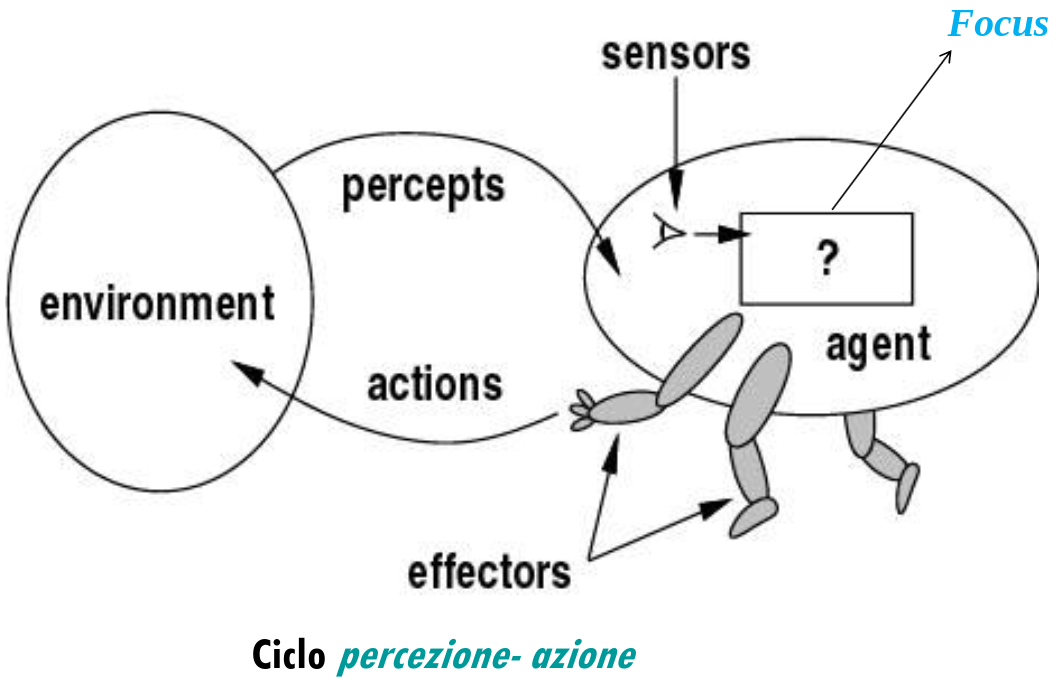
\includegraphics[scale=0.25]{images/agente.png}
\end{center}
Noi ci concentreremo sul programma che sta al centro dell'agente e che consiste in un ciclo di percezione-azione.
\subsection{Caratteristiche}
Un agente ha alcune caratteristiche:
\begin{itemize}
	\item \textbf{Situati}: ricevono \emph{percezioni} da un ambiente e agiscono mediante \textbf{azioni} (attuatori)
	
\end{itemize}

\subsubsection{Percezioni e azioni}
Le percezioni corrispondono agli \textbf{input} dai sensori. La \textbf{sequenza percettiva} sarà la storia completa delle percezioni.\\
La scelta dell'azione è \emph{funzione} unicamente della sequenza percettiva ed è chiamata \textbf{funzione agente}.\\
Il compito dell'IA è costruire il programma agente.
\begin{center}
	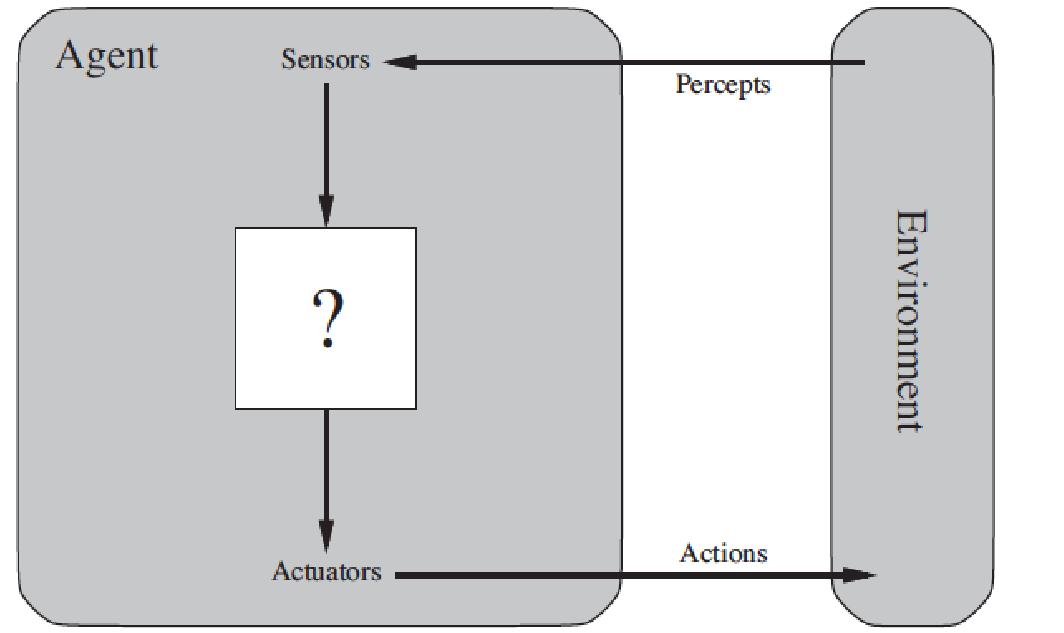
\includegraphics[scale=0.2]{images/architettura_astratta.png}
	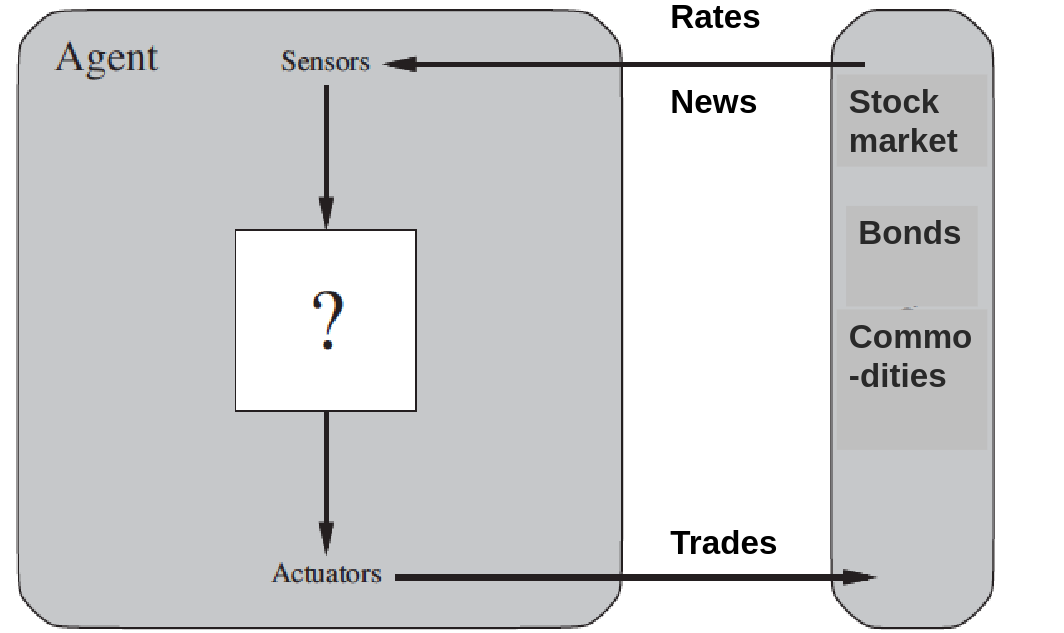
\includegraphics[scale=0.2]{images/agente_finanziario.png}
\end{center}
%TODO Caption

\subsection{Agente razionale}
Un agente razionale interagisce con il suo ambiente in maniera \textbf{efficace} (fa la cosa giusta).
Si rende quindi necessario un \textbf{criterio di valutazione} oggettivo dell'effetto delle azioni dell'agente. La valutazione della prestazione deve avere le seguenti caratteristiche:
\begin{itemize}
	\item Esterna (come vogliamo che il mondo evolva?)
	\item Scelta dal progettista a seconda del problema considerando l'effetto desiderato sull'ambiente.
	\item (possibile) Valutazione su ambienti diversi.
\end{itemize}
\begin{definition}[Agente razionale]
	Per ogni sequenza di percezioni compie l’azione che massimizza il valore atteso della
	misura delle prestazioni, considerando le sue percezioni passate e la sua conoscenza pregressa.
\end{definition}
\begin{observation}
	Si basa sulla razionalità e non sull'onniscenza e onnipotenza: non conosce alla perfezione il futuro ma può apprendere e hai dei limiti nelle sue azioni.
\end{observation}

Raramente tutta la conoscenza sull’ambiente può essere fornita a priori dal programmatore. L’agente razionale deve essere in grado di modificare il proprio comportamento con l’esperienza. Può \textbf{migliorare} esplorando, apprendendo, aumentando l'autonomia per operare in ambienti differenti o mutevoli.

\begin{definition}[Agente autonomo]
	Un agente è autonomo nella misura in cui il suo comportamento dipende dalla sua
	capacità di ottenere esperienza e non dall’aiuto del progettista.
\end{definition}

\subsection{Ambienti}
Definire un problema per un agente significa innanzitutto caratterizzare l'ambiente in cui opera. Viene utilizzata la descrizione \textbf{PEAS}:
\begin{itemize}
	\item \textbf{P}erformance
	\item \textbf{E}nviroment
	\item \textbf{A}ctuators
	\item \textbf{S}ensors
\end{itemize}

\begin{center}
	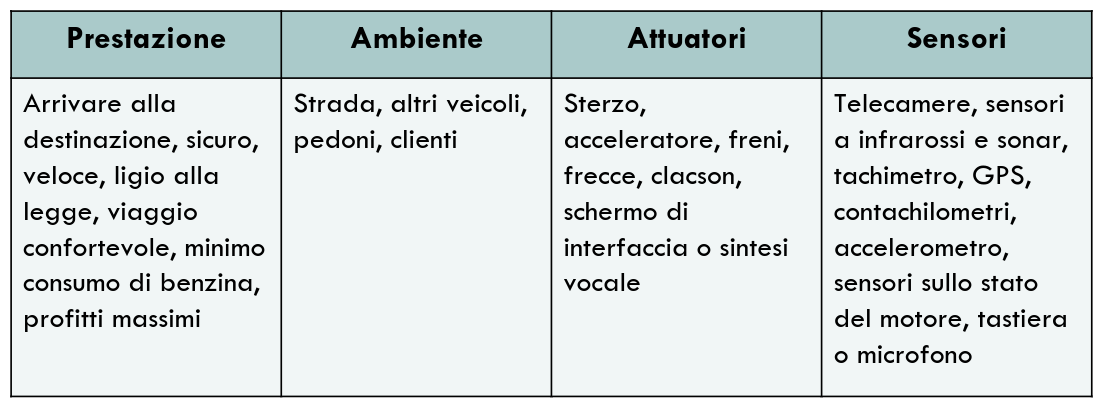
\includegraphics[scale=0.3]{images/agente_ambiente.png}
	%TODO Caption
\end{center}

L'ambiente deve avere le seguenti proprietà:
\begin{itemize}
	\item Osservabilità:
	\begin{itemize}
		\item Se è \textbf{completamente osservabile} l'apparato percettivo è in grado di dare conoscenza completa dell'ambiente o almeno tutto ciò che è necessario per prendere l'azione
		\item Se è \textbf{parzialmente osservabile} sono presenti limiti o inaccuratezze dell'apparato sensoriale
	\end{itemize}
	\item Agente singolo o multi-agente:
	\begin{itemize}
		\item L'ambiente ad agente \textbf{singolo} può anche cambiare per eventi, non
		necessariamente per azioni di agenti
		\item Quello \textbf{multi-agente} può essere \emph{competitivo} (scacchi) o \emph{cooperativo}
	\end{itemize}
	\item Predicibilità:
	\begin{itemize}
		\item \textbf{Deterministico}: quando lo stato successivo è completamente determinato dallo stato corrente e dall’azione (e.g. scacchi)
		\item \textbf{Stocastico}: quando esistono elementi di incertezza con associata probabilità (e.g. guida)
		\item \textbf{Non deterministico}: quando si tiene traccia di più stati possibili risultato dell’azione ma non in base ad una probabilità
	\end{itemize}
\end{itemize}
\newpage
\begin{itemize}
	\item Episodico o sequenziale:
	\begin{itemize}
		\item \textbf{Episodico}: quando l’esperienza dell’agente è divisa in episodi atomici
		indipendenti in cui non c'è bisogno di pianificare (e.g. partite diverse)
		\item \textbf{Sequenziale}: quando ogni decisione influenza le successive (e.g. mosse di scacchi)
	\end{itemize}
	\item Statico o dinamico:
	\begin{itemize}
		\item \textbf{Statico}: il mondo non cambia mentre l’agente decide l’azione (e.g cruciverba)
		\item \textbf{Dinamico}: cambia nel tempo, va osservata la contingenza e tardare equivale a non agire (e.g. taxi)
		\item \textbf{Semi-dinamico}: l’ambiente non cambia ma la valutazione dell’agente sì (e.g. scacchi con timer)
	\end{itemize}
	\item Valori come lo stato, il tempo, le percezioni e le azioni possono assumere valori \textbf{discreti} o \textbf{continui}. Il problema è combinatoriale nel discreto o infinito nel continuo.
	\item \textbf{Noto} o \textbf{ignoto}: una distinzione riferita alla conoscenza dell'agente sulle leggi fisiche dell'ambiente (le regole del gioco). È diverso da osservabile.
\end{itemize}

\begin{definition}[Simulatore]
	Un simulatore è uno strumento software che si occupa di:
	\begin{itemize}
		\item Generare stimoli
		\item Raccogliere le azioni in risposta
		\item Aggiornare lo stato
		\item Attivare altri processi che influenzano l'ambiente
		\item Valutare la prestazione degli agenti (media su più istanze)
	\end{itemize}
	Gli esperimenti su classi di ambienti con condizioni variabili sono essenziali per \textbf{generalizzare}.
\end{definition}

\subsection{Programma agente}
L'agente sarà quindi composto da un'architettura e da un programma. Il programma dell'agente implementa la funzione agente $Ag: Percezioni \to Azioni$. 

\begin{lstlisting}
	function Skeleton-Agent (percept) returns action
		static: memory, agent memory of the world
		memory <- UpdateMemory(memory, percept)
		action <- Choose-Best-Action(memory)
		memory <- UpdateMemory(memory, action)
		return action
\end{lstlisting}

\subsubsection{Tabella}
Un agente basato su tabella esegue una scelta come un accesso ad una tabella che associa un'azione ad ogni possibile sequenza di percezioni.\\
Ha una \textbf{dimensione ingestibile}, è difficile da costruire, non è autonomo ed è di difficile aggiornamento (apprendimento complesso).

\subsubsection{Agenti reattivi}
L'agente agisce in base a quello che percepisce senza salvare nulla in memoria.
\begin{center}
	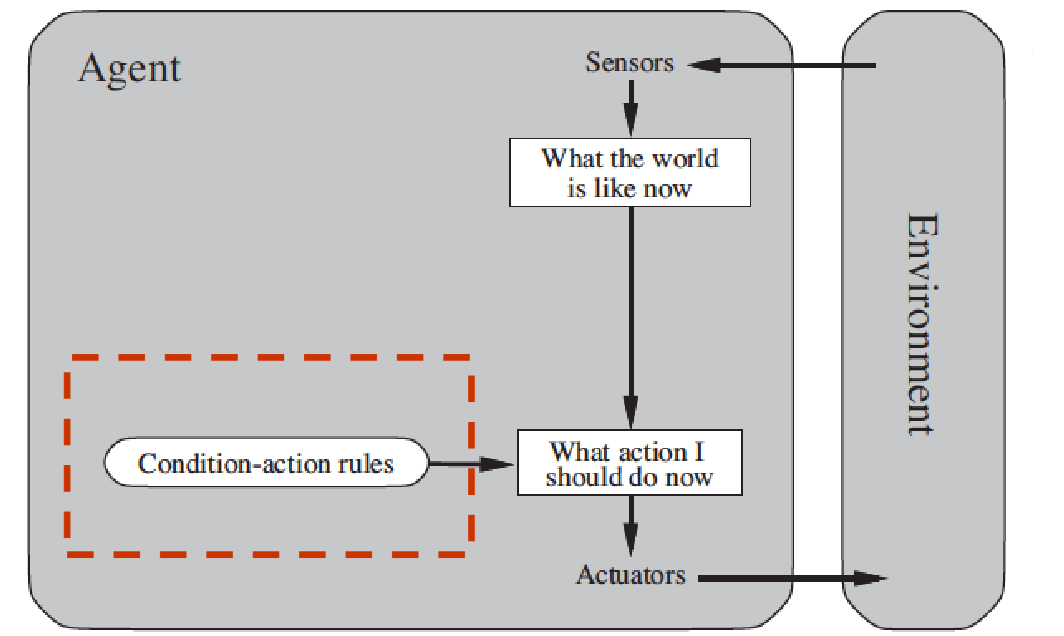
\includegraphics[scale=0.25]{images/agenti_reattivi.png}
\end{center}
\begin{lstlisting}
	function Agente-Reattivo-Semplice (percezione)
		returns azione
		persistent: regole, un insieme di regole
		condizione-azione (if-then)
		stato <- Interpreta-Input(percezione)
		regola <- Regola-Corrispondente(stato, regole)
		azione <- regola.Azione
		return azione
\end{lstlisting}

\subsubsection{Agenti basati su modello}
L'agente ha uno stato che mantiene la storia delle percezioni e influenza il modello del mondo.
\begin{center}
	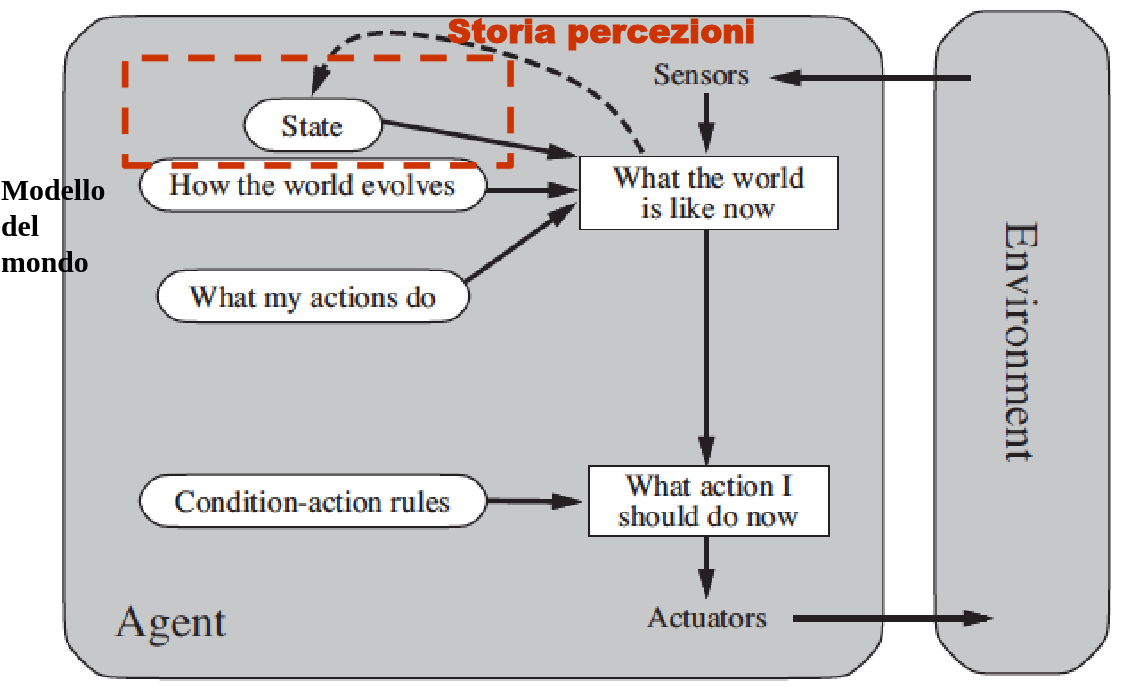
\includegraphics[scale=0.25]{images/agenti_modello.png}
\end{center}
\begin{lstlisting}
	function Agente-Basato-su-Modello (percezione)
		returns azione
		persistent: stato, una descrizione dello stato corrente
								modello, conoscenza del mondo
								regole, un insieme di regole condizione-azione
								azione, azione piu recente
		stato <- Aggiorna-Stato(stato, azione, percez., modello)
		regola <- Regola-Corrispondente(stato, regole)
		azione <- regola.Azione
		return azione
\end{lstlisting}

\subsubsection{Agenti con obiettivo}
Fin'ora l'agente aveva un obiettivo predeterminato dal programma. In questo caso invece viene specificato anche il \textbf{goal} che influenza le azioni. Abbiamo quindi più \textbf{flessibilità} ma meno efficienza.
\begin{center}
	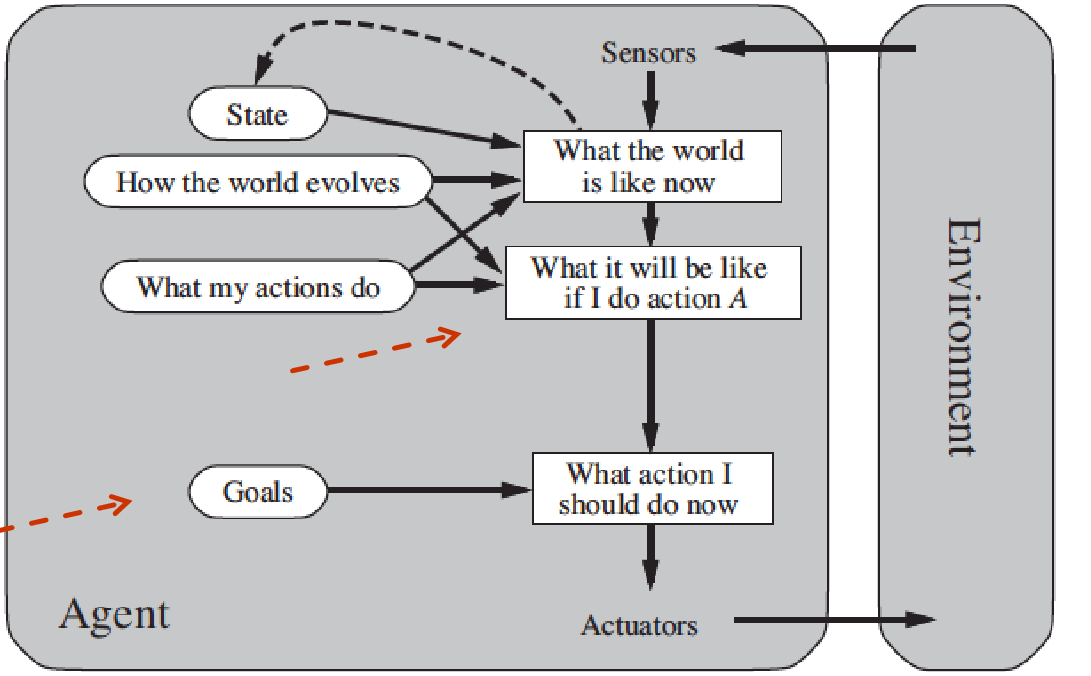
\includegraphics[scale=0.25]{images/agenti_obiettivo.png}
\end{center}

\subsubsection{Agenti con valutazione di utilità}
In questo caso ci sono \textbf{obiettivi alternativi} o più modi per raggiungerlo. L'agente deve quindi decidere verso dove muoversi e si rende necessaria una \textbf{funzione utilità} che associ ad un obiettivo un numero reale. La funzione terrà anche conto della probabilità di successo (\textbf{utilità attesa}).
\begin{center}
	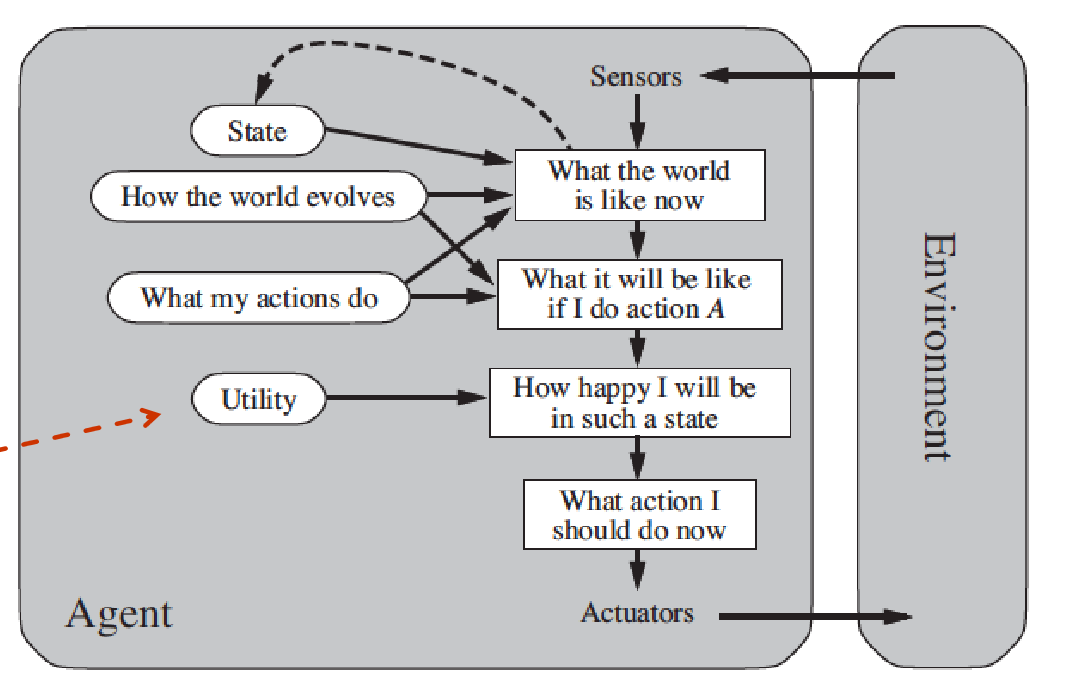
\includegraphics[scale=0.25]{images/agenti_utilita.png}
\end{center}

\subsubsection{Agenti che apprendono}
Questo tipo di agente include la capacità di \textbf{apprendimento} che produce cambiamenti al programma e ne migliora le prestazioni, adattando i comportamenti.\\
L'elemento \textbf{esecutivo} è il programma stesso, quello \textbf{critico} osserva e dà feedback ed infine c'è un generatore di problemi per suggerire nuove situazioni da esplorare.
\begin{center}
	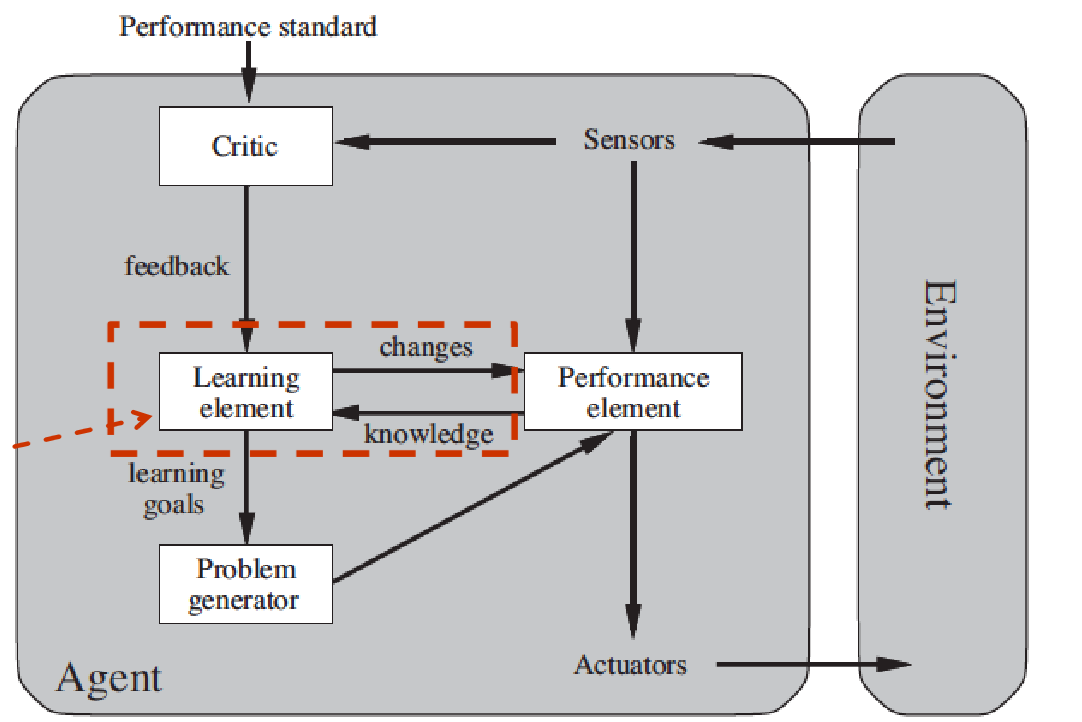
\includegraphics[scale=0.25]{images/agenti_apprendono.png}
\end{center}

\subsubsection{Tipi di rappresentazione}
Gli stati e le transizioni possono essere rappresentati in tre modi:
\begin{itemize}
	\item \textbf{Atomica}: solo con gli stati
	\item \textbf{Fattorizzata}: con più variabili e attributi
	\item \textbf{Strutturata}: con l'aggiunta delle relazioni
\end{itemize}
\begin{center}
	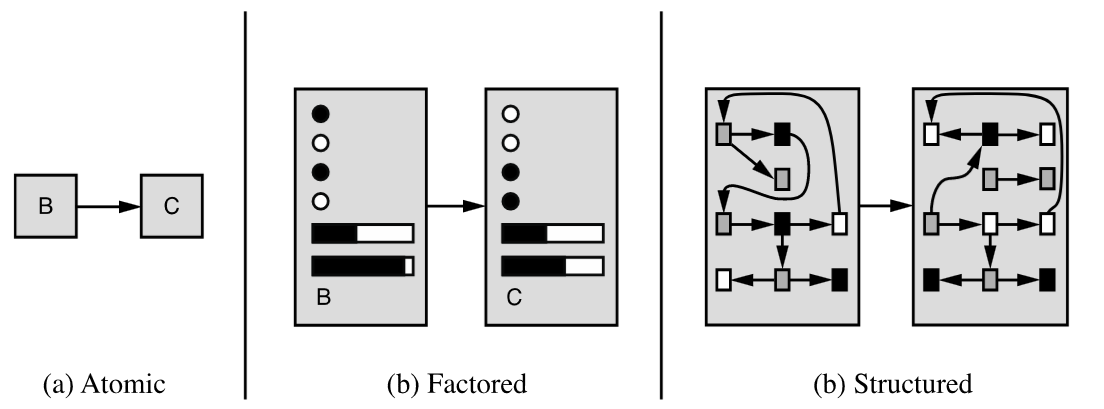
\includegraphics[scale=0.35]{images/rappresentazioni.png}
\end{center}
	% !TeX spellcheck = it_IT
\newpage
\section{Agenti risolutori di problemi}
Gli agenti risolutori di problemi adottano il paradigma della risoluzione di problemi come \textbf{ricerca} in uno \textbf{spazio di stati}. Sono agenti con \textbf{modello} (storia percezioni e stati) che adottano una rappresentazione \textbf{atomica} degli stati.\\
Sono particolari gli agenti con \textbf{obiettivo} che pianificano l'intera sequenza di mosse prima di agire.

\subsection{Processo di risoluzione}
I passi da seguire sono i seguenti:
\begin{enumerate}
	\item \textbf{Determinazione di un obiettivo}, ovvero un insieme di stati in cui l'obiettivo è soddisfatto
	\item \textbf{Formulazione} del problema tramite la rappresentazione degli stati e delle azioni
	\item Determinazione della \textbf{soluzione} mediante la ricerca
	\item \textbf{Esecuzione} del piano
\end{enumerate}

\begin{example}[Viaggio con mappa]
	Supponiamo di voler fare un viaggio. Il processo di risoluzione sarebbe il seguente:
	\begin{enumerate}
		\item Raggiungere Bucarest
		\item \begin{itemize}
			\item Azioni: guidare da una città all'altra
			\item Stato: città su mappa
		\end{itemize}
	\end{enumerate}
\end{example}

\subsection{Assunzioni}
Assumiamo che l'ambiente in questione sia \textbf{statico}, \textbf{osservabile}, \textbf{discreto} e \textbf{deterministico} (assumiamo un mondo ideale).

\subsection{Formulazione del problema}
Un problema può essere definito formalmente mediante 5 componenti:
\begin{enumerate}
	\item \textbf{Stato iniziale}
	\item \textbf{Azioni} possibili
	\item \textbf{Modello di transizione}: $ris: stato \times azione \to stato$, uno stato \emph{successore} $ris(s,a)=s'$
	\item \textbf{Test obiettivo} per capire tramite un insieme di stati obiettivo se il goal è raggiunto $test: stato \to \{true,false\}$
	\item \textbf{Costo del cammino}: composto dalla somma dei costi delle azioni, dove un passo ha costo $c(s,a,s')$. Un passo non ha mai costo negativo.
\end{enumerate}
I punti 1, 2 e 3 definiscono implicitamente lo \textbf{spazio degli stati}. Definirlo esplicitamente può essere molto costoso.

\subsection{Algoritmo di ricerca}
Gli algoritmi di ricerca prendono in input un problema e restituiscono un \textbf{cammino soluzione}.\\
Dobbiamo misurare le \textbf{prestazioni}: trova una soluzione? Quanto costa trovarla? Quanto è efficiente?
\begin{equation*}
	costo\_totale=costo\_ricerca+costo\_cammino\_sol
\end{equation*}

\begin{example}[Arrivare a Bucarest]
	Partiamo con la formulazione del problema:
	\begin{enumerate}
		\item \textbf{Stato iniziale}: la città di partenza, ovvero Arad
		\item \textbf{Azioni}: spostarsi in una città collegata vicina
		\begin{lstlisting}
			Azioni(In(Arad))={Go(Sibiu),Go(Zerind),...}
		\end{lstlisting}
		\item \textbf{Modello di transizione}: 
		\begin{lstlisting}
			Risultato(In(Arad), Go(Sibiu)) = In(Sibiu)
		\end{lstlisting}
		\item \textbf{Test obiettivo}:
		\begin{lstlisting}
			{In(Bucarest)}
		\end{lstlisting}
		\item \textbf{Costo del cammino}: somma delle lunghezze delle strade
	\end{enumerate}
	In questo esempio lo spazio degli stati coincide con la rete dei collegamenti tra le città.
	\begin{center}
		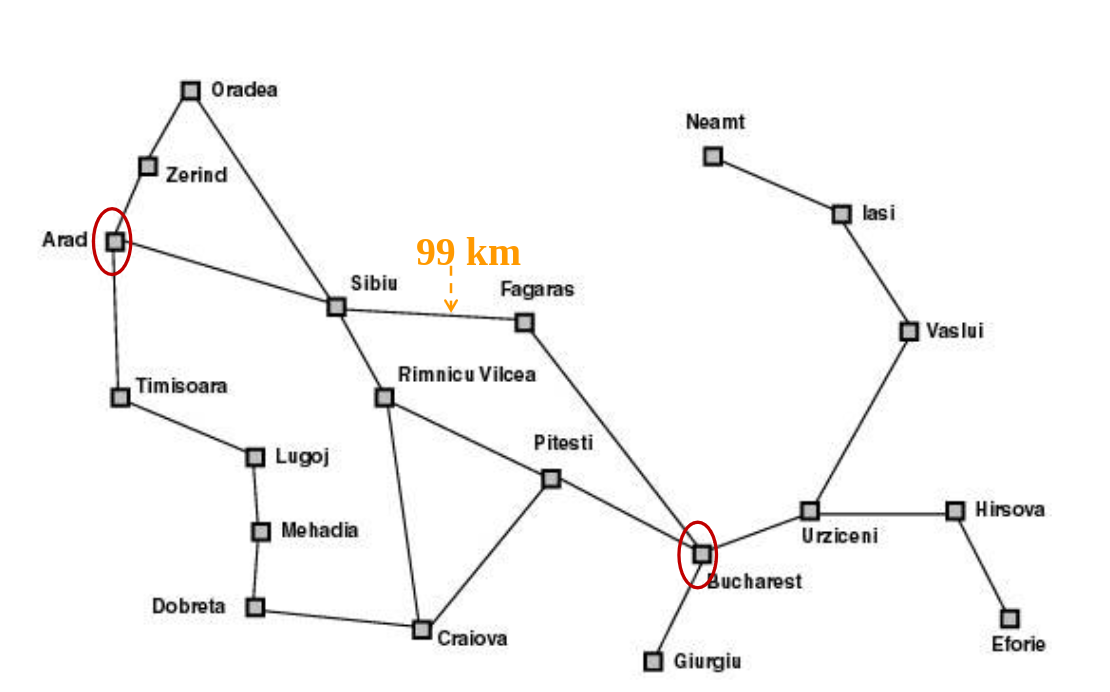
\includegraphics[scale=0.2]{bucarest_example.png}
	\end{center}
\end{example}

\begin{example}[Puzzle dell'8]
	Partiamo con la formulazione del problema:
	\begin{enumerate}
		\item \textbf{Stati}: tutte le possibili configurazioni della scacchiera
		\item \textbf{Stato iniziale}: una configurazione tra quelle possibili
		\item \textbf{Obiettivo}: una configurazione del tipo
		\begin{center}
			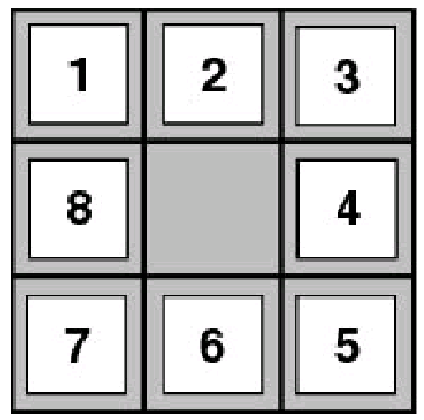
\includegraphics[scale=0.2]{8_puzzle_win.png}
		\end{center}
		\item \textbf{Azioni}: le mosse della casella vuota
		\item \textbf{Costo cammino}: ogni passo costa 1
	\end{enumerate}
	In questo esempio lo spazio degli stati è un grafo con possibili cicli (ci possiamo ritrovare in configurazioni già viste). Il problema è NP-completo: per 8 tasselli ci sono $\frac{9!}{2}=181.000$ stati.
\end{example}

\begin{example}[8 regine]
	Supponiamo di dover collocare 8 regine su una scacchiera in modo tale che nessuna regina sia attaccata da altre.
	\begin{enumerate}
		\item \textbf{Stati}: tutte le possibili configurazioni della scacchiera con 0-8 regine
		\item \textbf{Goal test}: avere 8 regine sulla scacchiera, di cui nessuna è attaccata
		\item \textbf{Azioni}: aggiungi una regina
	\end{enumerate}
	In questo esempio lo spazio degli stati sono le possibili scacchiere, ovvero $64 \times 63 \times \ldots \times 57 \simeq 1.8 \times 10^{14}$.\\
	Proviamo ad utilizzare una formulazione diversa:
	\begin{enumerate}
		\item \textbf{Stati}: tutte le possibili configurazioni della scacchiera in cui \emph{nessuna regina è minacciata}
		\item \textbf{Goal test}: avere 8 regine sulla scacchiera, di cui nessuna è attaccata
		\item \textbf{Azioni}: aggiungere una regina nella colonna vuota più a destra ancora libera in modo che non sia minacciata
	\end{enumerate}
	Lo spazio degli stati passa a $2057$, anche se comunque rimane esponenziale per $k$ regine.\\
	Vediamo infine un'ultima formulazione:
	\begin{enumerate}
		\item \textbf{Stati}: scacchiere con 8 regine, una per colonna
		\item \textbf{Goal test}: nessuna delle regine già presenti è attaccata
		\item \textbf{Azioni}: sposta una regina nella colonna se minacciata
		\item \textbf{Costo cammino}: zero
	\end{enumerate}
	Qui lo spazio degli stati è di qualche decina di milione.\\
	Capiamo quindi che formulazioni diverse del problema portano a spazi di stati di dimensioni diverse.
\end{example}

\begin{example}[Dimostrazione di teoremi]
	Dato un insieme di premesse:
	\begin{equation}
		\{s, t, q \Rightarrow p, r \Rightarrow p, v \Rightarrow q, t \Rightarrow r, s \Rightarrow v\}
	\end{equation}
	dimostrare una proposizione $p$ utilizzando solamente la regola di inferenza \emph{Modus Ponens}:
	\begin{equation*}
		(p \wedge p\Rightarrow q) \Rightarrow q
	\end{equation*}
	Scriviamo la formulazione del problema:
	\begin{itemize}
		\item \textbf{Stati}: insieme di proposizioni
		\item \textbf{Stato iniziale}: le premesse
		\item \textbf{Stato obiettivo}: un insieme di proposizioni contenente il teorema da dimostrare
		\item \textbf{Operatori}: l'applicazione del Modus Ponens
	\end{itemize}
	Lo spazio degli stati è quindi il seguente:
	\begin{center}
		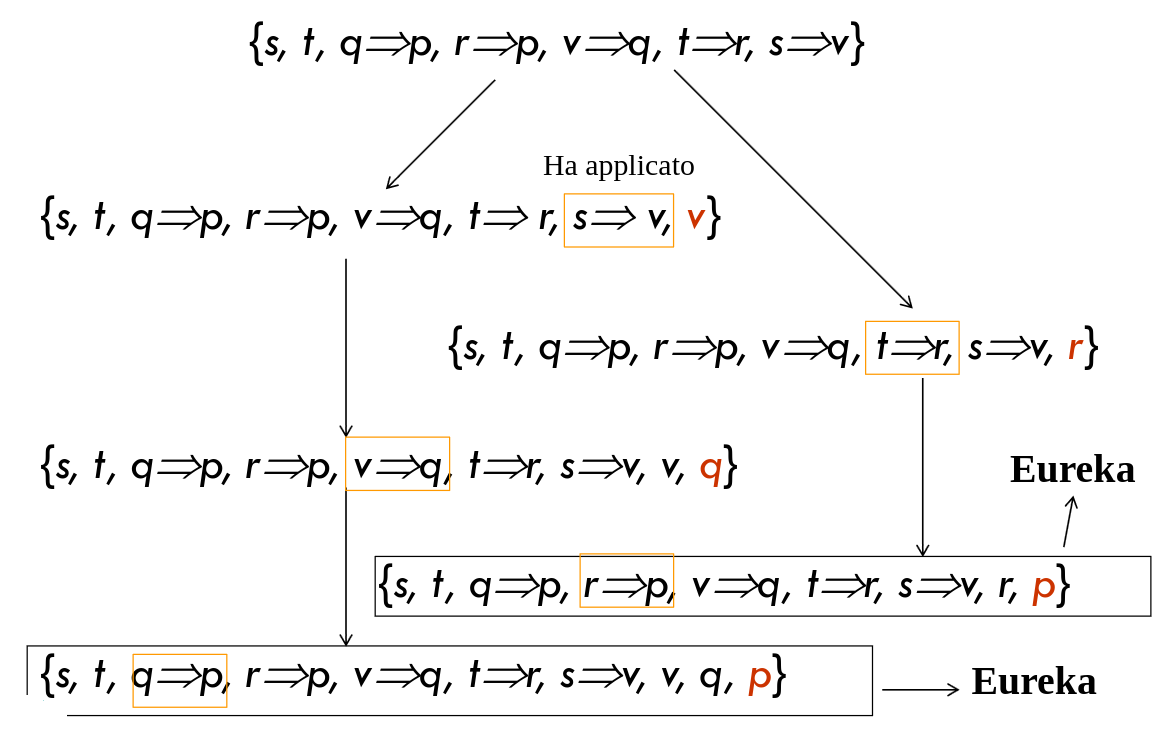
\includegraphics[scale=0.3]{dimostrazione_teoremi.png}
	\end{center}
\end{example}

%TODO Spostare da qui in poi in un altro file
\subsection{Ricerca della soluzione}
La ricerca della soluzione consiste nella generazione di un \textbf{albero di ricerca} a partire dalle possibili sequenze di azioni che si sovrappone allo spazio degli stati.\\
Ad esempio per il caso di Bucarest:
\begin{center}
	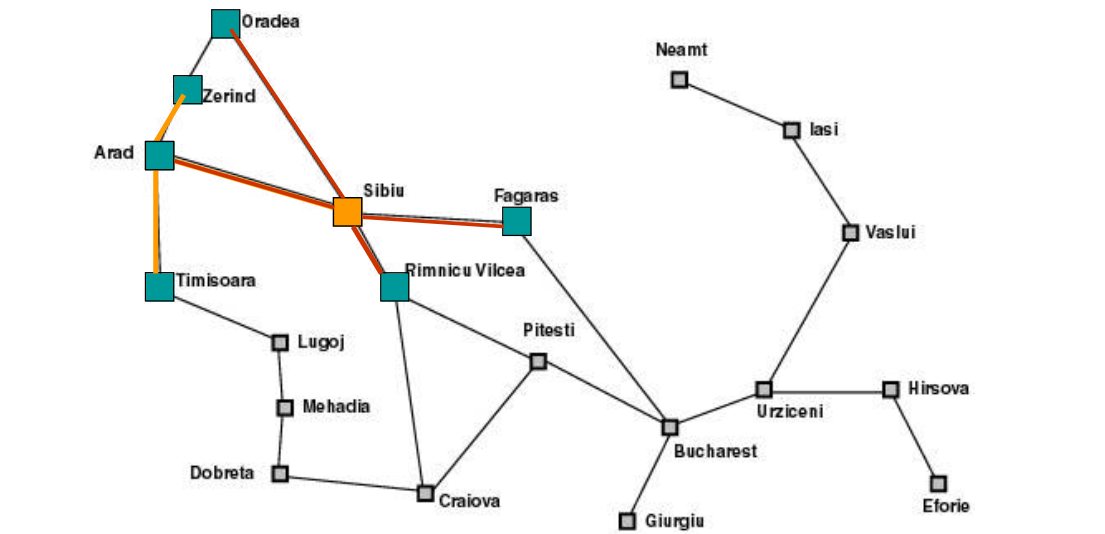
\includegraphics[scale=0.3]{bucarest_tree.png}
\end{center}
Espandiamo ogni nodo con i suoi possibili successori (frontiera).
\begin{definition}[Frontiera]
	Lista dei nodi in attesa di essere espansi (le foglie dell'albero di ricerca).
\end{definition}
\begin{observation}
	Si noti che un nodo dell'albero è diverso da uno stato. Infatti possono esitere nodi dell'albero di ricerca con lo stesso stato (si può tornare indietro).
\end{observation}

\subsection{Strategie di ricerca}
Ci sono diversi tipi di strategia per la ricerca della soluzione:
\begin{itemize}
	\item \textbf{FIFO}
	\item \textbf{LIFO}
	\item \textbf{Coda con priorità}
\end{itemize}

%TODO Ti sei perso delle slide

\subsubsection{Breadth First}
Come esplorare il grafo dello spazio degli stati a livelli progressivi di stessa profondità.\\
Per ogni nodo lo espandiamo, analizziamo i suoi figli (senza scendere ulteriormente di livello) e dopo averli fatti tutti scende di livello seguendo il principio FIFO.\\
Il seguente è il codice della \textbf{ricerca ad albero}, ovvero dove non si torna su un nodo già visitato.

\begin{lstlisting}
	function Ricerca-Ampiezza-A
		returns soluzione oppure fallimento
		nodo = un nodo con stato il problema.stato-iniziale e costo-di-cammino=0
		if problema.Test-Obiettivo(nodo.Stato) then return Soluzione(nodo)
		frontiera = una coda FIFO con nodo come unico elemento
	loop do
		if Vuota?(frontiera) then return fallimento
		nodo = POP(frontiera)
		for each azione in problema.Azioni(nodo.Stato) do
		figlio = Nodo-Figlio(problema, nodo, azione) [costruttore: vedi AIMA]
		if Problema.TestObiettivo(figlio.Stato) then return Soluzione(figlio)
		frontiera = Inserisci(figlio, frontiera) /* frontiera gestita come coda FIFO
	end
\end{lstlisting}

Il seguente è invece quello della \textbf{ricerca su grafo}:
\begin{lstlisting}
	function Ricerca-Ampiezza-g
		returns soluzione oppure fallimento
		nodo = un nodo con stato il problema.stato-iniziale e costo-di-cammino=0
		if problema.Test-Obiettivo(nodo.Stato) then return Soluzione(nodo)
		frontiera = una coda FIFO con nodo come unico elemento
		esplorati = insieme vuoto
	loop do
		if Vuota?(frontiera) then return fallimento
		nodo = POP(frontiera); aggiungi nodo.Stato a esplorati
		for each azione in problema.Azioni(nodo.Stato) do
		figlio = Nodo-Figlio(problema, nodo, azione)
		if figlio.Stato non e in esplorati e non in frontiera then
		if Problema.TestObiettivo(figlio.Stato) then return Soluzione(figlio)
		frontiera = Inserisci(figlio, frontiera) /* in coda
	end
\end{lstlisting}

\noindent Analizziamone la complessità partendo dalle seguenti assunzioni:
\begin{itemize}
	\item Fattore di \textbf{branching} $b$: numero massimo di successori
	\item \textbf{Depth} del nodo obiettivo più superficiale
	\item Lunghezza \textbf{massima} dei cammini nello spazio degli stati
\end{itemize}
La strategia è ottimale se tutti gli operatori hanno lo stesso costo $k$, ovvero se $g(n)=k \cdot depth(n)$, dove $g(n)$ è il costo del cammino per arrivare ad $n$.\\
La complessità nel \emph{tempo} (nodi generati) sarà 
\begin{equation*}
	T(b,d)=1+b+b^2+\ldots+b^d \longrightarrow O(b^d)
\end{equation*}
mentre in \emph{spazio} (nodi in memoria):
\begin{equation*}
	O(b^d)
\end{equation*}
È chiaro che l'algoritmo scali male, sopratutto per quanto riguarda lo spazio.

\subsubsection{Depth first}
In questo algoritmo si parte da un nodo e si scende nel primo figlio, procedendo appunto in profondità. Arrivati alle foglie si torna indietro ai figli precedentemente non visitati. In memoria tengo solamente  i fratelli del path corrente ed elimino i rami già esplorati.\\  Possono esserci tre versioni possibili:
\begin{itemize}
	\item \textbf{Albero}: data $m$ la lunghezza massima dei cammini nello spazio degli stati e $b$ il fattore di diramazione, la \textbf{complessità} in \emph{tempo} è $O(b^m)$ (può essere maggiore di $O(b^d)$) mentre in \emph{spazio} è $b \cdot m$.
	Rispetto al Breadth First, non è né completo né ottimale, ma ci garantisce un notevole risparmio in memoria
	\item \textbf{Grafo}: la memoria corrisponde a tutti i possibili stati, diventando quindi completo nello spazio finito (non in quello infinito)
	\item \textbf{Ricorsiva}: ancora più efficiente per la memoria perché mantiene solo il cammino corrente ($O(m)$). Viene realizzata con un algoritmo di \emph{backtracing} che salva lo stato su uno stack a cui torna in caso di fallimento.
\end{itemize}
\newpage
\begin{lstlisting}
	function Ricerca-DF-A (problema)
		returns soluzione oppure fallimento
		return Ricerca-DF-ricorsiva(CreaNodo(problema.Stato-iniziale), problema)
	
	function Ricerca-DF-ricorsiva(nodo, problema)
		returns soluzione oppure fallimento
		if problema.TestObiettivo(nodo.Stato) then return Soluzione(nodo)
		else
		for each azione in problema.Azioni(nodo.Stato) do
			figlio = Nodo-Figlio(problema, nodo, azione)
			risultato = Ricerca-DF-ricorsiva(figlio, problema)
			if risultato != fallimento then return risultato
		return fallimento
\end{lstlisting}
\subsubsection{Depth Limited}
La ricerca in profondità limitata arriva fino ad un dato livello $l$. È completa solo se si conosce il limite superiore $d$ per la profondità della soluzione e $d<l$. Non è ottimale e ha complessità in tempo $O(b^l)$ e in spazio $O(b \cdot l)$
\subsubsection{Iterative Depth}
Questo approccio prevede di provare l'algoritmo depth limited con limite di profondità $l=0, 1, \ldots$ fino a trovare la soluzione. È il miglior compromesso tra breadth first e depth first:
\begin{itemize}
	\item Complessità in \textbf{tempo} $O(b^d)$ se ammette soluzione
	\item Complessità in \textbf{spazio} $O(b \cdot d)$ se ammette soluzione
\end{itemize}
Quindi ha la \emph{completezza} e l'\emph{ottimalità} del breadth first e la complessità in \emph{spazio} della depth first.
\subsubsection{Uniform Cost}
Partendo da una ricerca in ampiezza, la generalizziamo: si sceglie il nodo di costo minore sulla frontiera e si espande sui contorni di costo uguale.
\begin{center}
	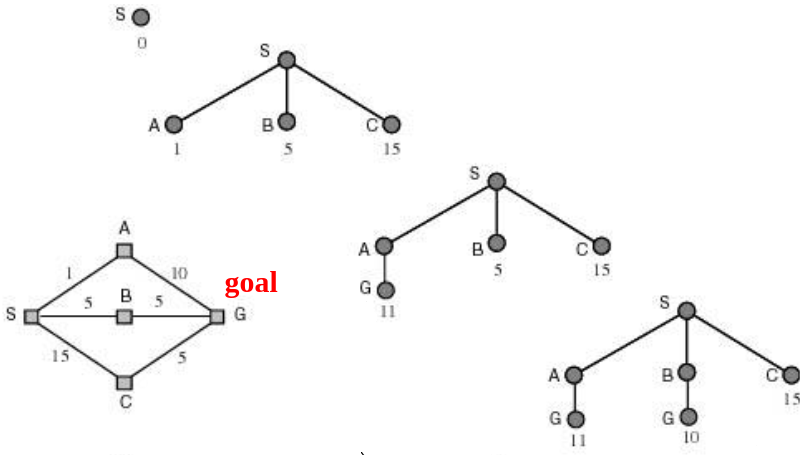
\includegraphics[scale=0.4]{uc.png}
\end{center}
\newpage
Codice per la ricerca su albero:
\begin{lstlisting}
	function Ricerca-UC-A (problema)
			returns soluzione oppure fallimento
			nodo = un nodo con stato il problema.stato-iniziale e costo-di-cammino=0
			frontiera = una coda con priorita con nodo come unico elemento
		loop do
			if Vuota?(frontiera) then return fallimento
			nodo = POP(frontiera)
			if problema.TestObiettivo(nodo.Stato) then return Soluzione(nodo)
			for each azione in problema.Azioni(nodo.Stato) do
				figlio = Nodo-Figlio(problema, nodo, azione)
				frontiera = Inserisci(figlio, frontiera) /* in coda con priorita*/
	end
\end{lstlisting}
Codice per la ricerca su grafo:
\begin{lstlisting}
	function Ricerca-UC-G (problema)
			returns soluzione oppure fallimento
			nodo = un nodo con stato il problema.stato-iniziale e costo-di-cammino=0
			frontiera = una coda con priorita con nodo come unico elemento
			esplorati = insieme vuoto
		loop do
			if Vuota?(frontiera) then return fallimento
			nodo = POP(frontiera);
			if problema.TestObiettivo(nodo.Stato) then return Soluzione(nodo)
			aggiungi nodo.Stato a esplorati
			for each azione in problema.Azioni(nodo.Stato) do
				figlio = Nodo-Figlio(problema, nodo, azione)
				if figlio.Stato non in esplorati e non in frontiera then
					frontiera = Inserisci(figlio, frontiera) /* in coda con priorita
				else if figlio.Stato in frontiera con Costo-cammino piu alto then
					sostituisci quel nodo frontiera con figlio */
	end
\end{lstlisting}
Questo algoritmo è \textbf{ottimo} e \textbf{completo} purché il costo degli archi sia $\epsilon > 0$. Assunto $C^*$ come costo della soluzione ottima, $\lfloor \frac{C^*}{\epsilon}\rfloor$ è il numero di mosse nel caso peggiore. La complessità è quindi $O(b^{1+\lfloor \frac{C^*}{\epsilon}\rfloor})$.
\begin{note}
	Quando ogni azione ha lo stesso costo, la complessità si avvicina a quella della breadth first: $O(b^{1+d})$.
\end{note}
\subsection{Direzione}
Un problema importante è quello della \textbf{direzione} della ricerca, che può essere:
\begin{itemize}
	\item In \textbf{avanti} o guidata da \emph{dati}: si esplora lo spazio di ricerca dallo stato iniziale all'obiettivo
	\item All'\textbf{indietro} o guidata dall'\emph{obiettivo}: si esplora lo spazio di ricerca partendo da uno stato goal e riconducendosi ad un sotto-goal fino a trovare uno stato iniziale
\end{itemize}
Per scegliere la direzione bisogna tenere in conto di quale ha il \textbf{fattore di diramazione} minore.  Si preferisce la ricerca all'\emph{indietro} quando l'obiettivo è ben definito (e.g. theorem proving) mentre quella in \emph{avanti} quando ci sono molteplici obiettivi (e.g. design).\\
\subsubsection{Ricerca bidirezionale}
Nella ricerca bidirezionale si procede in entrambe le direzioni fino ad incontrarsi. La \textbf{complessità} è:
\begin{itemize}
	\item \emph{Tempo}: $O(\sqrt{b^d})$ assumendo che il test dell'intersezione delle due direzioni sia costante
	\item \emph{Spazio}: $O(\sqrt{b^d})$, poiché almeno tutti i nodi di una direzione saranno in memoria
\end{itemize}
Si noti che non sempre è applicabile, come nel caso in cui i predecessori non siano definiti o ci siano troppi stati obiettivo.

\subsection{Problematiche}
\subsubsection{Cicli}
I cammini ciclici rendono gli alberi di ricerca \emph{infiniti} anche quando lo spazio degli stati è finito.
\begin{center}
	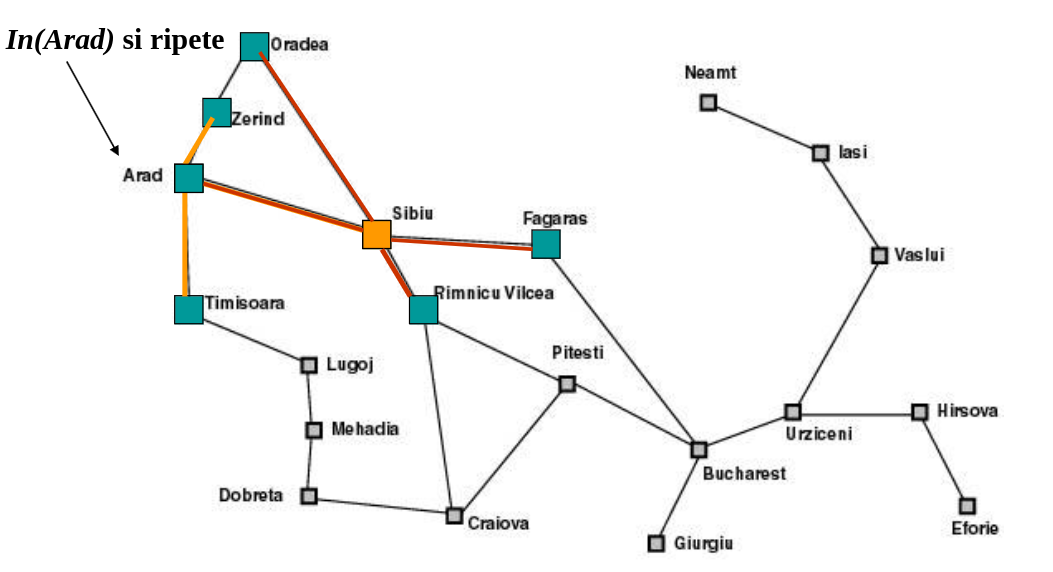
\includegraphics[scale=0.4]{cicli.png}
\end{center}
\subsubsection{Ridondanze}
Su spazi di stati a grafo si possono generare più volte nodi con lo stesso stato nella ricerca, anche in assenza di cicli.
\begin{center}
	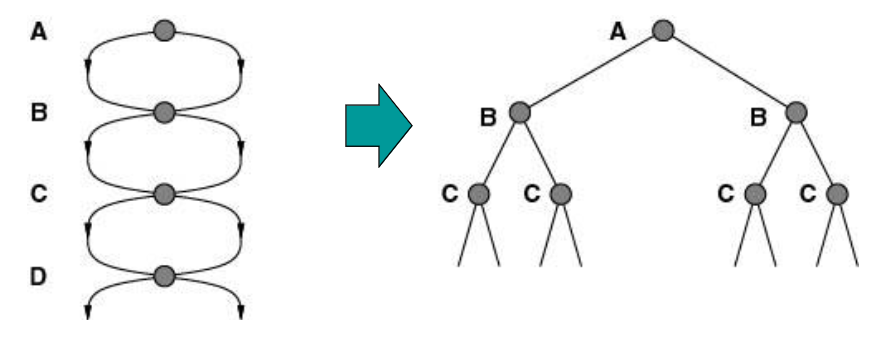
\includegraphics[scale=0.4]{ridondanze.png}
\end{center}
Visitare questi stati è lavoro inutile. Per evitarlo serve \textbf{ricordare} gli stati già visitati, occupando ovviamente più spazio. Tre possibili soluzioni sono:
\begin{enumerate}
	\item Non tornare nel nodo \textbf{genitore}, eliminandolo dai successori (non evita i cammini ridondanti)
	\item Per evitare i \textbf{cammini ciclici} si controlla che  i successori non siano antenati del nodo corrente
	\item Non generare nodi con \textbf{stati già esplorati}: ogni nodo visitato deve essere salvato in memoria
\end{enumerate}
Il costo può essere alto, ad esempio nella depth first la complessità in spazio torna ad essere pari a tutti gli stati.\\
La \textbf{ricerca} sul grafo avverrà quindi come segue:
\begin{enumerate}
	\item Mantiene una lista di stati esplorati (lista chiusa)
	\item Prima di espandere un nodo si controlla se era già stato incontrato o se è già nella frontiera
	\item In quel caso, non viene espanso
\end{enumerate}
Questa tecnica è ottimale solo se abbiamo la garanzia che il costo del nuovo cammino sia maggiore o uguale, ovvero non convenga.
\subsection{Confronto}
\begin{table}[!h]
	\centering
	\begin{tabular}{|c|c|c|c|c|c|c|}
		\hline
		\textbf{Confronto} & \textbf{BF} & \textbf{UC} & \textbf{DF} & \textbf{DL} & \textbf{ID} & \textbf{BDir}\\
		\hline
		Completa & Si & Si(*) & No & Si(**) & Si & Si(***)\\
		Tempo &$O(b^d)$ &$O(b^{1+\lfloor \frac{C^*}{\epsilon}\rfloor})$ & $O(b^m)$ & $O(b^l)$ & $O(b^d)$ & $O(\sqrt{b^d})$ \\
		Spazio &$O(b^d)$ &$O(b^{1+\lfloor \frac{C^*}{\epsilon}\rfloor})$ & $O(b\cdot m)$ & $O(b\cdot l)$ & $O(b\cdot d)$ & $O(\sqrt{b^d})$\\
		Ottimale & Si(****) & Si(*)& No & No & Si(****)& Si(***)\\
		\hline
	\end{tabular}
\end{table}
Legenda:
\begin{itemize}
	\item  \textbf{*}: se $\text{costo archi} \geq \epsilon \geq 0$
	\item \textbf{**}:  se si conosce il limite alla profondità della soluzione ($l>d$)
	\item \textbf{***}: se si utilizza UC o BF
	\item \textbf{****}: se gli archi hanno tutti lo stesso costo
\end{itemize}

	\newpage
\section{Ricerca euristica}
La ricerca esaustiva non è praticabile in problemi di complesità esponenziale (e.g. $10^{120}$ configurazioni in scacchi). Noi usiamo
conoscenza del problemi es esperienza per riconoscere i cammini più promettenti, usiamo una stima del costo futuro, evitando di generare gli altri.
La conoscenza euristica (dal greco "eureka") aiuta fare scelte "oculate", questa ovviamente però non evita la ricerca ma la riduce, consente in
genere di trovare una buona soluzione in tempi accettabilili sotto certe condizioni garantisce completezza e ottimalità.\\\\
La conoscenza del problema data tramite una funzione di valutazione $f$, che include $h$ detta \textbf{funzione di valutazione euristica}.
$$h: n \to R$$
La funzione si applica al nodo ma dipende solo dallo stato (n.Stato).
\begin{note}
    Manteniamo la notazione in $n$ per unifomritò con $g$; $g$ dipende anche dal cammino fino al nodo.
\end{note}
$$f(n) = g(n) + h(n) \text{ove g(n) è il costo cammino visto con UC}$$
Per procedere preferibilmente verso il percorso migliore, seguendo problem-specific information, di stima del costo futuro:
\begin{itemize}
    \item La città più vicina (o la città più vicina alla metà in linea d'aria - tabella esterna) nel problema dell'itinerario.
    \item Il numero della caselle fuori posto nel gioco dell'otto.
    \item Il vataggio in pezzi della dama o negli scacchi
\end{itemize}

\begin{example}
    Mappa Romania dist. in linea d'aria.
    \begin{figure}[h!]
        \centering
        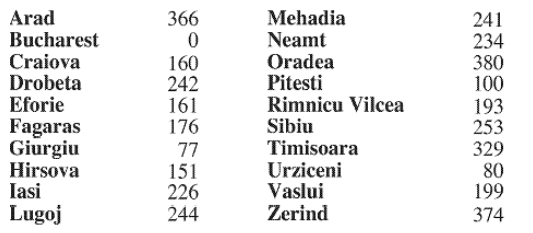
\includegraphics[width=0.75\textwidth]{images/esempio-euristica-h.png}
    \end{figure}
\end{example}

\subsection{Algoritmo di ricerca Best-first}
Il \textbf{best first - heuristic} usa lo stesso algoritmo di UC \footnote{Warning: AIMA ed. IV ha usato uno schema di
UC diverso e alcune proprietà cambiano} ma con uso di $f$ (stima di costo) per la coda con priorità.
Una volta scelta $f$ determina la strategia di ricerca. A ogni passo si sceglie il nodo sulla frontiera per cui il valore della $f$ è 
migliore (il nodo più promettente).
\begin{note}
    Migliore significa "minore" in caso di un'euristica che stima la distanza della soluzione
\end{note}
\hspace{-15pt}Un caso speciale: \textbf{greedy best-first}, su usa solo $h (f=h)$.
\begin{example}
    Esempio di greedy best-first con $f=h$
    \begin{figure}[h!]
        \centering
        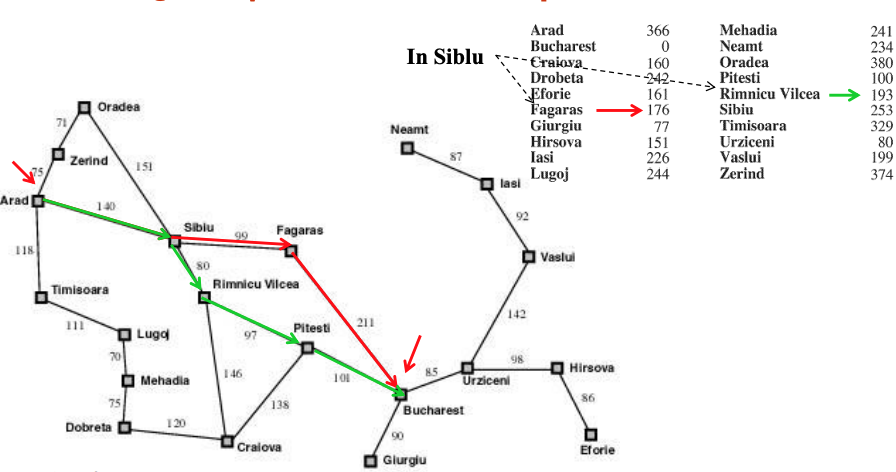
\includegraphics[width=0.75\textwidth]{images/esempio-best-first.png}
    \end{figure}
    Da Arad a Bucarest con \textbf{Greedy best-first}: Arad, sibiu, fagaras, bucharest (450) ma non è l'ottimale
    che sarebbe: Arad, Sibiu, Rimnicu, Pitesti, Bucarest (418).
\end{example}

\subsection{Algoritmo A}
Si può dire qualcosa di $f$ per avere garanzie di completezza e ottmialità?
\begin{definition}
    Un \textbf{Algoritmo A} è un algoritmo di best first con una fuzine di valutazione dello stato del tipo:
    $$f(n) = g(n) + h(n) \:\: \text{con}\:\: h(n) \geq 0 \:\: \text{e}\:\: h(goal) = 0$$
\end{definition}
In questa definizione abbiamo che $g(n)$ è il costo del cammino percorso per raggiugnere n, mentre $h(n)$ una
stima del costo per raggiungere da n un nodo goal (distanza).\\
Vedremo alcuni casi particolari dell'algoritmo A:
\begin{itemize}
    \item Se $h(n) = 0 \:\:[f(n) = g(n)]$ si ha \textbf{Ricerca Uniforme (UC)}.
    \item Se $g(n) = 0 \:\:[f(n) = h(n)]$ si ha \textbf{Greedy Best First}.
\end{itemize}
\begin{example}
    Esempio nel gioco dell'otto.
    \begin{figure}[h!]
        \centering
        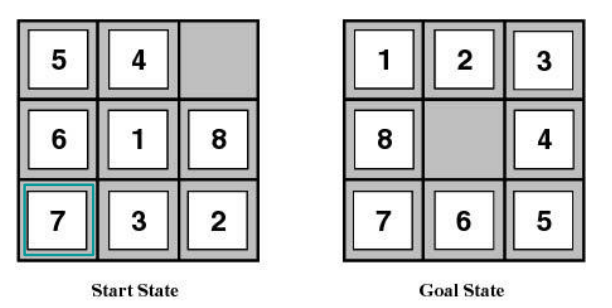
\includegraphics[width=0.6\textwidth]{images/esempio-gioco-otto.png}
    \end{figure}

    \hspace{-15pt}$f(n) = \#\text{mosse fatte} \:\: + \:\: \#\text{caselle-fuori-posto} \hspace{10pt} f(start) = 0 + 7 \hspace{10pt} f(goal-state) = ? + 0$\\
    Dopo $\leftarrow, \downarrow, \uparrow, \rightarrow$ abbiamo che $f = 4 + 7$, stesso stato, $g$ è cambiato.
\end{example}
\begin{theorem}
    L'algoritmo A con la condizione:
    $$g(n) \geq d(n) \cdot \epsilon \hspace{10pt}(\epsilon >0 \text{ costo minimo arco})$$
    è completo (con $d(n)$ che è la distanza).
\end{theorem}
\begin{note}
    La conzione ci garantisce che non si verifichino situazioni strane del tipo:
    \begin{figure}[h!]
        \centering
        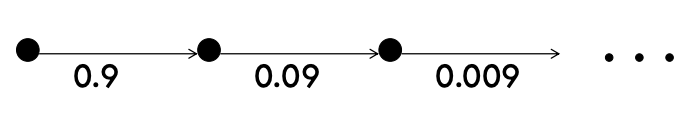
\includegraphics[width=0.65\textwidth]{images/nota-alg-completo.png}
    \end{figure}
    e quindi che il costo lungo un cammino non cresca "abbastanza" (se cresce abbastanza possiamo fermare quel path per costo alto di g).
\end{note}
\begin{demostration}
    Sia $[n_0, n_1, n_2, \dots, n', \dots, n_k = goal]$ un cammino soluzione. Sia $n'$ un nodo della frontiera su un cammino soluzione:
    $n'$ prima o poi sarà espanso. Infatti esistono solo un numero finito di nodi $x$ che possono essere aggiunti alla frontiera con $f(x) \leq f(n')$
    (è la condizione sulla crescita di g, scritta precedentemetne, tale che non esista una catena infinita di archi e nodi che possa aggiungere con costo sempre $\leq f(n')$).\\\\
    Quindi, se non si trova una soluzione prima, $n'$ verrà espanso e i suoi successori aggiunti alla frontiera. Tra questi anche il suo successore sul cammino soluzione.\\
    Il ragionamento si può ripetere fino a dimostrare che anche il nodo goal sarà selezionato per l'espanzione.
\end{demostration}

\subsection{Algoritmo $A^*$}
La funzione di valutazione ideale (oracolo):
$$f^*(n) = g^*(n) + h^*(n)$$
Con $g^*(n)$ il costo del cammino minimo da radice a n, $h^*(n)$ costo del cammino minimo da n a goal, $f^*(n)$ costo
del cammino minimo da radice a goal, attraverso n. Normalmente:
$$g(n) \geq g^*(n) \hspace{10pt} e \hspace{10pt} h(n) \text{ è una stima di } h^*(n)$$
($g(n) \geq g^*(n)$ rappresenta costo cammino $\geq$ costo migliore). Si può andare in sottostima (e.g. linea d'aria) o 
sovrastima della distanza dalla soluzione.
\begin{definition}[Euristica ammissibile]
    $$\forall n\:\: t.c.\:\: h(n) \leq h^*(n) \:\:\:\: \text{h è una sottostima}$$
\end{definition}
\begin{example}
    L'euristica della distanza in linea d'aria.
\end{example}
\begin{definition}[Algoritmo $A^*$]
    Un algoritmo A in cui h è una funzione euristica ammissibile.
\end{definition}
\begin{theorem}
    Gli algoritmi $A^*$ sono \textbf{ottimali}.
\end{theorem}
\begin{corollaries}
    $BF^{(+)}$ e UC sono ottimali ($h(n) = 0$).
\end{corollaries}
\begin{example}
    Itinerario con $A^*$ (ad albero).
    \begin{figure}[h!]
        \centering
        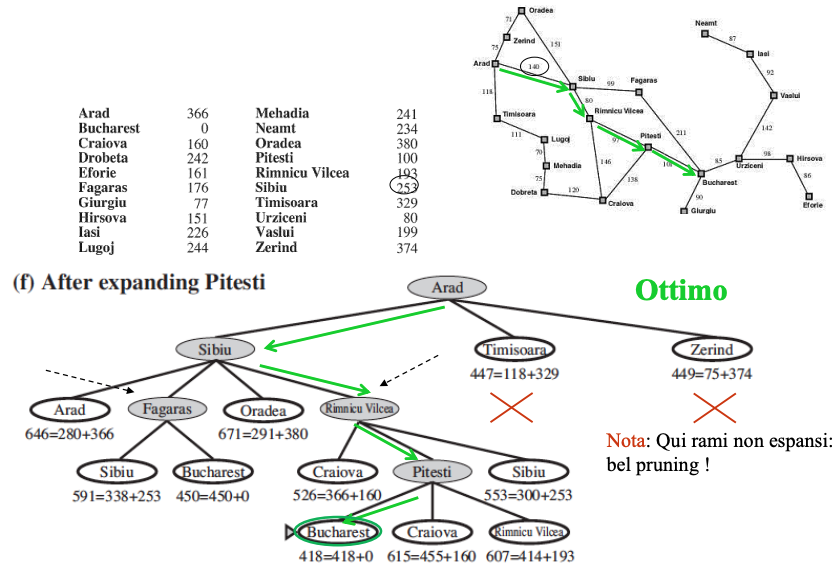
\includegraphics[width=0.62\textwidth]{images/itinerario-A*-albero.png}
    \end{figure}
\end{example}
\begin{observation}
    Alcune osservazioni su $A^*$
    \begin{enumerate}
        \item Rispetto a greedy best-first, la componente g fa si che si abbandonino cammini che vanno troppo in profondità.
        \item Ha sotto o sovra stima?
        \begin{enumerate}
            \item Una sottostima (h) può farci compiere del lavoro inutile (tenendo anche candidati non buoni), però non ci 
            fa perdere il cammino migliore (quando prendo nodo goal è il cammino migliore).
            \item Una funzione che qualche volta sovrastima può farci perdere la soluzione ottimale (taglio per causa di sovrastima, invece era buona)
        \end{enumerate}
    \end{enumerate}
\end{observation}

\subsubsection{Ottimalità su $A^*$}
\begin{wrapfigure}[8]{r}{5cm}
    \vspace{-30pt}
    \centering
    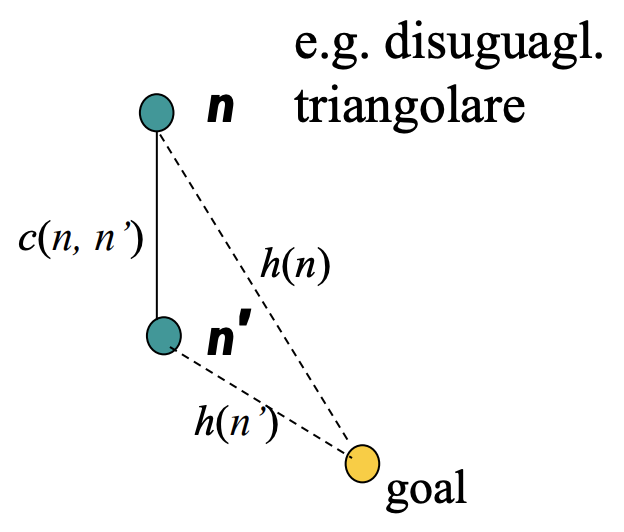
\includegraphics[width=4cm]{images/dis-triagolare.png}
\end{wrapfigure}
Nel caso di ricerca a/su albero l'uso di un'euristica ammissibile è sufficente a garantire l'ottimalità su $A^*$.
Nel caso di ricerca su grafo (con UC come visto) serve una proprietà più forte: la \textbf{consistenza} (detta anche \textbf{monotonicità}).\\\\
Per evitare rischio di scartare candidati ottimi (stato già incontrato) si vuol evitare, causa uso della lista esplorati, di far sparire, o meglio
non considerare al momento dell'espansione, candidati ottimali. Cerchiamo quindi condizioni per garantire che il primo espanso sia il migliore.

\begin{definition} 
    Un euristica \textbf{consistente} $[h(goal) = 0]$ (consistenza locale).
    $$\forall n \:\: t.c. \:\: h(n) \leq c(n, a, n') + h(n') \text{ dove n' è un successore di n}$$
\end{definition}
\hspace{-15pt}Ne segue che $f(n) \leq f(n')$
\begin{note}
    Se h è consistente la $f$ non decresce mai lungo i cammini, da cui il termine \textbf{monotona}.
\end{note}
\begin{theorem}
    Un'euristica monotona è ammissibile.
\end{theorem}
\hspace{-15pt}Esistono euristiche ammissibili che non sono monotone, ma sono rare. Le euristiche monotone garantiscino che la soluzione meno costosa 
venga trovata per rima e quindi sono ottimali anche nel caso di ricerca su grafo.\\
Non si devono recuperare tra gli antenati nodi con costo minore. Lista degli esplorati, stato già esplorato è sul cammino ottimo allora posso
evitare di inserire il corrente ripetuto senza perdere l'ottimalità.
\begin{lstlisting}
    if figlio.Stato non e in esplorati e non e in frontiera then
        frontiera = Inserisci(figlio, frontiera)
\end{lstlisting}
Per la frontiera, volendo evitare stati ripetuti, resta 'if' finale di UC:
\begin{lstlisting}
    if figlio.Stato e in frontiera con Costo-cammino piu alto then
        sostituisci quel nodo frontiera con figlio 
\end{lstlisting}
Andiamo ora a verificare l'ottimalità di $A^*$ supponendo di avere il teorema, con $h$ consistente.
\begin{enumerate}
    \item Se $h(n)$ è consistente i valori di $f(n)$ lungo un cammino sono non decrescenti:
    $$\text{se } h(n) \leq c(n, a, n') + h(n') \hspace{10pt} \Rightarrow \text{(def. consistenza sommando g(n))}\hspace{10pt} g(n) + h(n) \leq g(n) + c(n, a, n') + h(n')$$
    ma siccome abbiamo $g(n) + c(n, a, n') = g(n')$ allora
    $$g(n) + h(n) \leq g(n') + h(n') \Rightarrow f(n) \leq f(n') \Rightarrow f \text{ monotona}$$
    \item Ogni volta che $A^*$ seleziona un nodo (n) per l'espansione, il cammino ottimo a tale nodo è stato trovato: 
    se così non fosse, ci sarebbe un altro nodo m ella frontiera sul cammino ottimo (a n, ancora da trovare con un cammino ottimo), con $f(m)$
    minore (per la monotonia e n successore di m); ma ciò non è possibile perché tale nodo sarebbe già stato espanso (si espande prima un nodo con f minore).
    \item Quando seleziona nodo goal è cammino ottimo $[h=0, f=C^*]$.
\end{enumerate}
% TODO: AGGIUNGI IMMAGINI
Quindi, detto questo, perché $A^*$ è vantaggioso?
\begin{itemize}
    \item $A^*$ espande tutti i nodi con $f(n) < C^*$ ($C^*$ = costo ottimo)
    \item $A^*$ espande alcuni nodi con $f(n) = C^*$.
    \item \textbf{$A^*$ non espande alcun nodo con $f(n) > C^*$}
\end{itemize}
Quindi alcuni nodi (e suoi sottoalberi) non verranno considerati per l’ espansione (ma restiamo ottimali):
pruning (h opportuna, più alta possibile tra le ammissibili, fa tagliare molto).\\\\
% TODO: AGGIUNGI IMMAGINE
Più f è aderente a stima ottimale, più taglio! Ovali più stretti. Cercheremo quindi una h il più alta possibile tra le ammissibili
Se molto bassa molti (sino a tutti i) nodi restano minore di $C^* \to$ espando tutti (a cerchi).
Il pruning sotto-alberi è il punto focale: non li abbiamo già in memoria e evitiamo di generarli (decisivo per i problemi di AI a spazio stati esponenziali.\\\\
In riassunto L’algoritmo è quello degli schemi usati per UC, Usando f = g+h per la coda con priorità, ove h e g soddisfano quanto allo slide 9 [A], 
ove h è una funzione euristica ammissibile $[A^*]$, e considerando le condizioni dette per ottenere l’ottimalità su grafi.
\begin{itemize}
    \item $A^*$ è \textbf{completo}: discende dalla completezza di A ($A^*$ è un algoritmo A particolare).
    \item $A^*$ con euristica monotona è \textbf{ottimale}.
    \item $A^*$ è \textbf{ottimamente efficiente}: a parità di euristica nessn altro algoritmo espande meno nodi (senza rinunciare a ottimalità)
\end{itemize}
I problemi principali sono la scelta dell'euristica e  ancora l'occupazione di memoria che nel caso
pessimo resta esponenziale come visto per gli altri algoritmi di ricerca con stesso schema, causa frontiera.

\subsection{Sotto-casi speciali: US e Greedy Best First}
Ci sono due casi particolai dell'algoritmo A:
\begin{enumerate}
    \item Se $h(n) = 0$ $[f(n) = g(n)]$ si ha Uniform Cost (UC), ossia $g$ non basta (si può migliorare).
    \item Se $g(n) = 0$ $[f(n) = h(n)]$ si ha Greedy Best Fist, ossia $h$ non basta (già visto all'inizio).
\end{enumerate}
\subsubsection{UC vs $A^*$}
Illustrazione dell'algoritmo di ricerca Dijkstra per trovare il percorso da un nodo iniziale (in basso
sinistra, rosso) a un nodo obiettivo (in alto a destra, verde) in un problema di pianificazione del movimento del robot.
I nodi aperti rappresentano l'insieme "provvisorio". I nodi pieni sono quelli visitati, con colore
che rappresenta la distanza: più verde, più lontano. Nodi in tutti i diversi
le direzioni vengono esplorate in modo uniforme, apparendo come un fronte d'onda più o meno circolare
poiché l'algoritmo di Dijkstra utilizza un'\textbf{euristica identicamente uguale a 0}. $\to$ UC !\\\\
\begin{wrapfigure}[6]{r}{5cm}
    \vspace{-35pt}
    \centering
    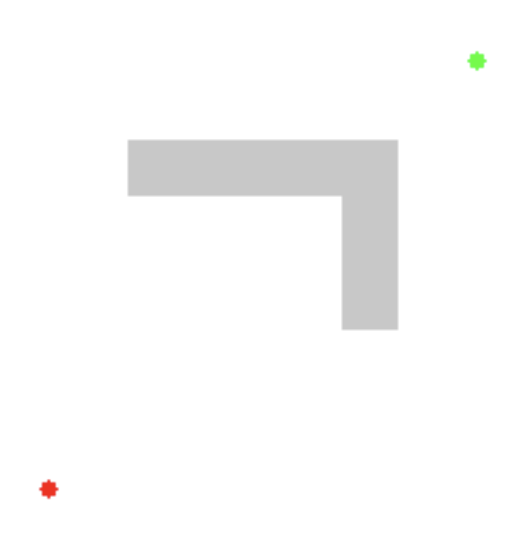
\includegraphics[width=3cm]{images/dijkstra.png}
\end{wrapfigure}
Illustrazione dell'algoritmo di ricerca A* per trovare il percorso da un nodo iniziale a un nodo obiettivo in un robot è un
problema di pianificazione del movimento. I cerchi vuoti rappresentano i nodi nell'insieme aperto, cioè,
quelli che restano da esplorare e quelli pieni sono nell'insieme chiuso. Colore acceso
ogni nodo chiuso indica la distanza dalla partenza: più è verde, più è lontano. Uno
può prima vedere A* muoversi in linea retta in direzione della porta, poi quando colpisce l'ostacolo, esplora percorsi alternativi attraverso i nodi da insieme aperto $\to$ frontiera.\\\\
L'algoritmo A* è una generalizzazione dell'algoritmo di Dijkstra che riduce le dimensioni del sottografo che deve essere esplorato, se il lower-bound
della "distanza" dall'obiettivo (h) è disponibile.

\subsection{Costruire le euristiche di $A^*$}
Partiamo dalle valutazione di funzioni euristiche. A parità di ammissibilità, una euristica può essere più
efficiente di un’altra nel trovare il cammino soluzione migliore (visitare meno nodi). Questo dipende da quanto
informata è l'euristia (dal \textbf{grado di informazione posseduto}) 
\begin{itemize}
    \item $h(n) = 0$ minimo di informazione (BF o UC)
    \item $h^*(n)$ massimo di infomrazione (oracolo)
\end{itemize}
In generale, per le euristiche ammissibili:
$$0 \leq h(n) \leq h^*(n)$$
\begin{theorem}
    Se $h_1 \leq h_2$, i nodi espansi\footnote{Ricorda che $A^*$ espande tutti i nodi con $f(n) = g(n) + h(n) < C^*$, e sono meno per $h$ maggiore (h maggiore fa andare più nodi oltre $C^*$).} da $A^*$ con $h_2$ sono un sottoinsieme di quelli espandi da $A^*$ con $h_1$.
\end{theorem}
\hspace{-15pt}Se $h_1 \leq h_2$, $A^*$ con $h_2$ è almeno efficiente quanto $A^*$ con $h_1$.
Un’euristica più informata (accurata) riduce lo spazio di ricerca (è più efficiente), ma è tipicamente più costosa da calcolare (e.g. un caso estremo ?)
\begin{example}
    Due euristiche ammissibili per il gioco dell'8 potrebbero essere le seguenti:
    \begin{itemize}
        \item $h_1$: conta il numero di caselle fuori posto
        \item $h_2$: somma delle distanze \textbf{Manhattan} (orizzonatle/verticale) delle caselle fuori posto dalla posizione finale.
    \end{itemize}
    $h_2$ è più informata di $h_1$, infatti $\forall n \:\:.\:\: h_1(n) \leq h_2(n)$, quindi si dice che $h_2$ \textbf{domina} $h_1$ (utile per confrontte tra ammissibili)
    \begin{figure}[h!]
        \centering
        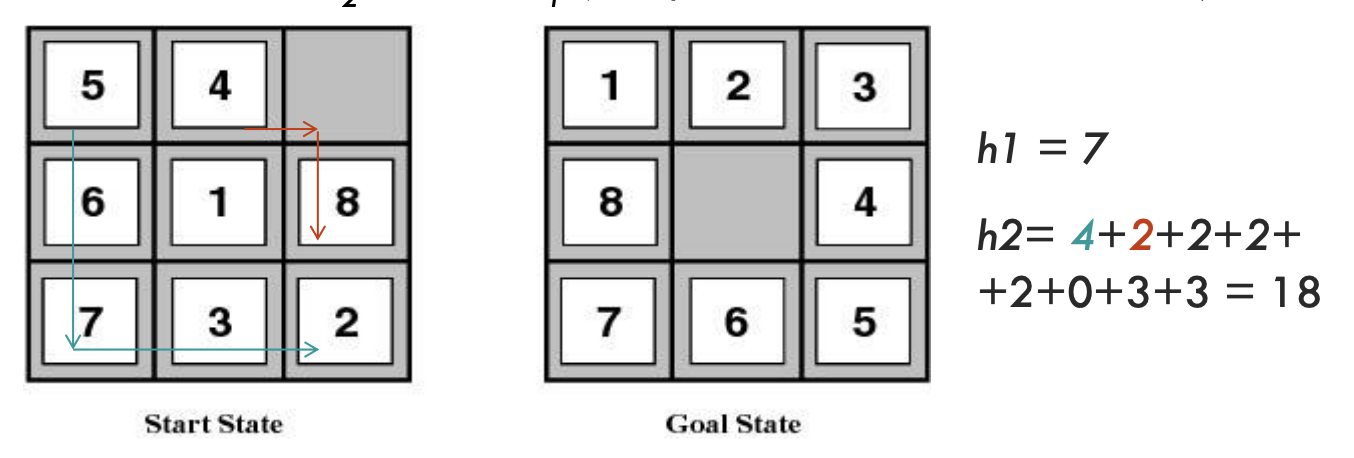
\includegraphics[width=0.65\textwidth]{images/euristica-gioco-8.png}
    \end{figure}
\end{example}
\begin{definition}
    La somma delle distanze Manghattan si definisce come:
    $$h((x,y)) = MD((x,y), (x_g, y_g)) = |x - x_g| + |y - y_g|$$
\end{definition}
\begin{figure}[h!]
    \centering
    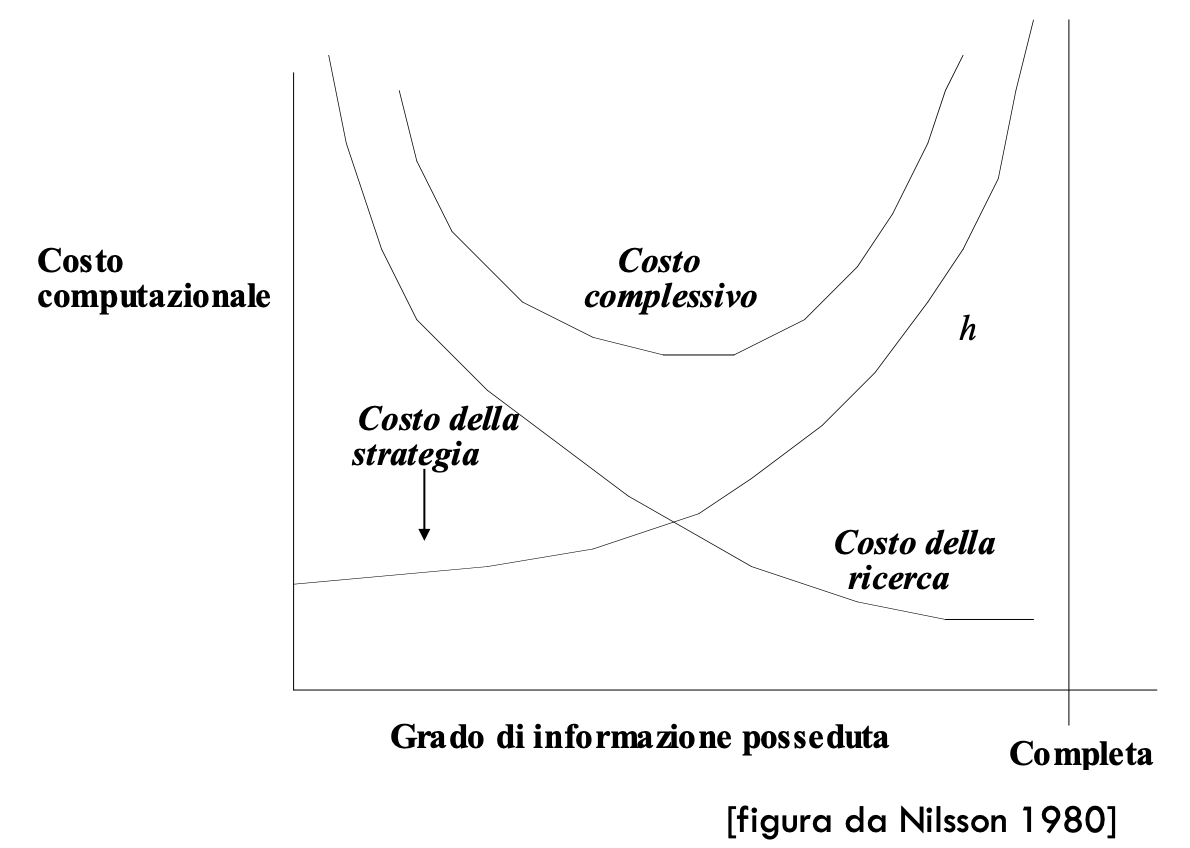
\includegraphics[width=0.60\textwidth]{images/costo-ricerva-vs-costo-euristica.png}
    \caption{Costo ricerca vs costo euristico}
\end{figure}
\hspace{-15pt}Ora capiamo come valutare gli algoritmi di ricerca euristica. Introfuciamo
il \textbf{fattore di diramazione effettivo} $b^*$, N: numero di nodi generati, d: profondità della soluzione.
$b^*$ è il fattore di diramazione di un albero uniforme con $N+1$ nodi, solizione dell'equazione:
$$N + 1 = b^* + (b^*)^2 + \dots + (b^*)^d$$
Sperimentalmente una buona euristica ha un $b^*$ abbastanza vicino a 1 (<1.5)
\begin{example}
    Ricodando l'esempio dal gioco dell'otto:
    \begin{figure}[h!]
        \centering
        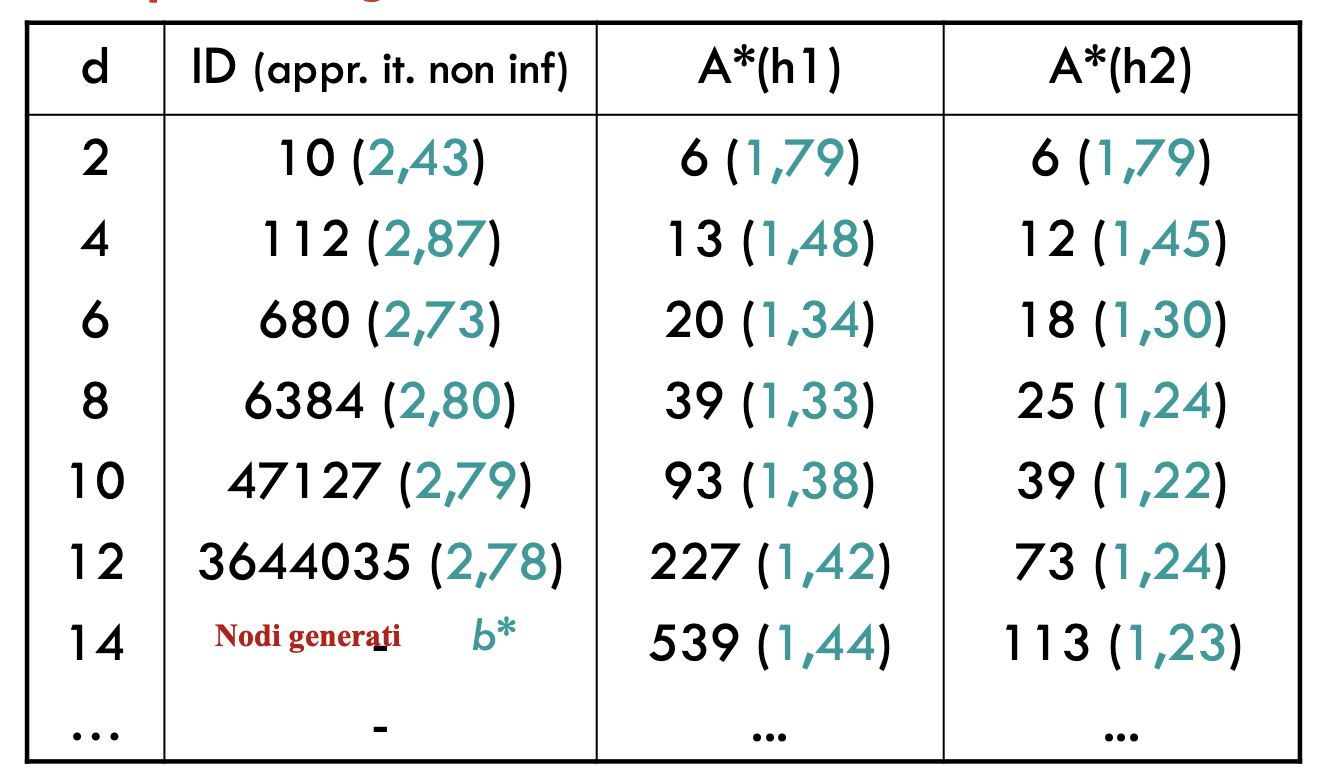
\includegraphics[width=0.60\textwidth]{images/gioco-otto-misura-euristiche.png}
    \end{figure}
    Sono riportati: Nodi generati e fattore di diramazione effettivo ($b^*$, verde)
    I dati sono mediati, per ogni d, su 100 istanze del problema [AIMA].\\\\
    Nella \textbf{capacità di esplorazione}, l'influenza di $b^*$:
    \begin{itemize}
        \item Con b=2: d=6 e N = 100 \hspace{15pt} d=12 e N = 10.0000
        \item Con b=1.5: d=12 N = 100 \hspace{15pt} d=24 e N = 10.000
    \end{itemize}
    migliorando di poco l’euristica si riesce, a parità di nodi espansi, a raggiungere una profondità doppia di esplorazione mosse!
\end{example}

\subsection{Inventare euristiche}
Quindi abbiamo che:
\begin{enumerate}
    \item Tutti i problemi dell’IA (o quasi) sono di complessità esponenziale ... (nel generare nodi, i.e. configurazioni possibili) ma c’è esponenziale e esponenziale!
    \item L’euristica può migliorare di molto la capacità di esplorazione dello spazio degli stati rispetto alla ricerca cieca.
    \item Migliorando anche di poco l’euristica si riesce ad esplorare uno spazio molto più grande (più in profondità).
\end{enumerate}
Per inventare un euristica ci sono alcune strategie, che aiutano appunto ad ottenre euristiche amissibili:
\begin{itemize}
    \item Rilassamento del problema
    \item Massimizzazione di euristiche
    \item Database di pattern disgiunti
    \item Combinazione lineare
    \item Apprendere dall’esperienza
\end{itemize} 
\subsubsection{Rillassamento problema}
\begin{example}
    Il rilassamento del problema nel gioco dell’8 mossa da A a B possibile se: 
    \begin{enumerate}
        \item \textbf{B adiacente a A}
        \item \textbf{B libera}
    \end{enumerate}
    $h_1$ e $h_2$ sono calcoli distanza esatta della soluzione in versioni semplificate del puzzle:
    \begin{itemize}
        \item $h_1$ (nessuna restrizione, ne 1 ne 2): sono sempre ammessi scambi a piacimento tra caselle (si muove
        ovunque) $\to$ numero caselle fuori posto.
        \item  $h_2$ (solo restrizione 1): sono ammessi spostamenti anche su caselle occupate, purché adiacenti $\to$ somma delle distanze Manhattan.
    \end{itemize}
\end{example}

\subsubsection{Massimizzazione di euristiche}
Se si hanno una serie di euristiche ammissibili $h_1, h_2, \dots, h_k$ \textbf{senza che nessuna "domini" un'altra}
allora conviene prendere il massimo dei lori valori:
$$h(n) = max(h_1(n), h_2(n), \dots, h_k(n))$$
Se le $h_i$ sono ammissibili, anche la $h$ lo è. La h domina tutte le altre.

\subsubsection{Database con pattern disgiunti}
\begin{figure}[h!]
    \centering
    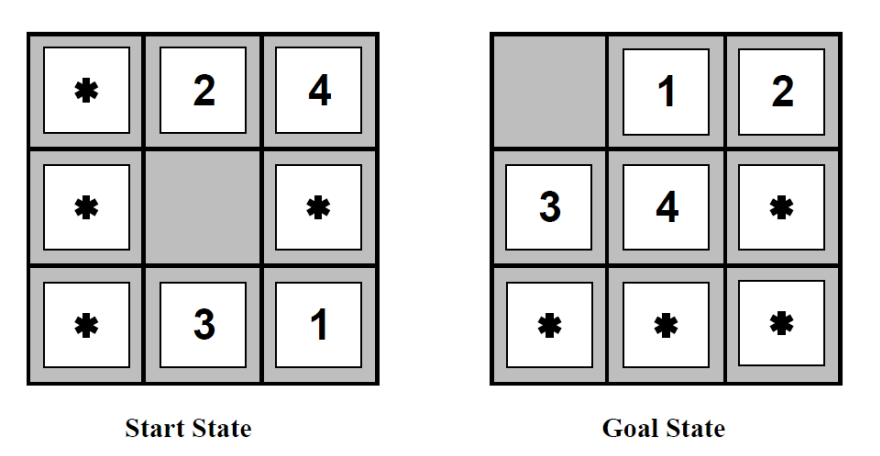
\includegraphics[width=0.65\textwidth]{images/euristiche-da-sottoproblemi.png}
\end{figure}
\hspace{-15pt}Costo della soluzione ottima al sottoproblema (di sistemare 1,2,3,4) è una sottostima del costo per il problema nel suo
complesso (e.g. rilevatesi più accurata della Manhattan). \\
\textbf{Database di pattern}: memorizzare ogni istanza del
sottoproblema con relativo costo della soluzione. Usare poi questo database per calcolare $h_{DB}$ (estraendo dal DB la
configurazione corrispondente allo stato completo corrente).
\begin{itemize}
    \item \textbf{Domanda}: Potremmo poi fare la stessa cosa per altri sottoproblemi: 5-6-7-8, 2-4-6-8, ottenendo altre euristiche ammissibili,
    poi prendere il valore massimo: ancora una euristica ammissibile. Ma potremmo sommarle e ottenere un’euristica
    ancora più accurata?
    \item \textbf{Risposta}: In generale no perché le soluzioni ai sottoproblemi interferiscono (condividono alcune mosse, se sposto 1-2-3-4, spostero
    anche 4-5-6-7) e la somma delle euristiche in generale non è ammissibile (potremmo sovrastimare avendo avuto aiuti mutui).
    Si deve eliminare il costo delle mosse che contribuiscono all’altro sottoproblema. Database di pattern disgiunti consentono di sommare i
    costi (euristiche additive) [e.g. solo costo mosse su1-2-3-4], sono molto efficaci: gioco del 15 in pochi ms
    ma per esempio difficile scomporre per cubo Rubik.
\end{itemize}

\subsubsection{Apprendimento dall'esperienza}
Bisogna eseguire un apprendimento dall'esperienza. Quindi far girare il programma, raccogliere dati: coppie
$<stato, h^*>$. Usare i dati per apprendere a predire la h con algoritmi di apprendimento induttivo (da istanze note stimiamo h in generale).\\
Gli algoritmi di apprendimento si concentrano su caratteristiche salienti dello stato (feature, xi) [e.g.
apprendiamo che da numero tasselli fuori posto 5 $\to$ costo~14, etc].

\subsubsection{Combinazione euristiche}
Quando diverse caratteristiche influenzano la bontà di uno stato, si può usare una combinazione lineare per combinare le euristiche:
$$h(n) = c_1 x_1(n) + c_2x_2(n) + \dots + c_k x_k(n)$$
\begin{example}
    Gioco dell'8: $h(n) = c_1 \:\: \#\text{fuori-posto} + c_2 \#\text{coppie-scambiate}$\\
    Scacchi: $h(n) = c_1 \:\text{vant-pezzi} + c_2 \:\text{pezzi-attacc.} + c_3 \:\text{regina} + \dots$
\end{example}
\hspace{-15pt}Il peso dei coefficienti può essere aggiustato con l’esperienza, anche qui apprendendo automaticamente da esempi di gioco.
$h(goal) = 0$ (e.g. gioco dell’8) ma ammissibilità e consistenza non automatiche.

\subsection{Algoritmi evoluti basati su $A^*$}
Ci sono una serie di algoritmi basati su $A^*$ che possono andare a portare ad un miglioramento dell'occupazione della memoria.
Fra questi abbiamo: Beam search, A* con approfondimento iterativo (IDA*), ricerca best-first ricorsiva (RBFS), A* con memoria limitata (MA*) in versione semplice (SMA*).

\subsubsection{Beam search}
Nel Best First viene tenuta tutta la frontiera; se l’occupazione di memoria è eccessiva si può ricorrere ad una variante: la Beam search.
La Beam Search tiene ad ogni passo solo i k nodi più promettenti, dove k è detto l’ampiezza del raggio
(beam). La Beam Search non è completa.

\subsubsection{IDA${}^*$}
L'$IDA^*$ è un $A^*$ con approfondimento iterativo. IDA* combina A* con ID: ad ogni iterazione si ricerca
in profondità con un limite (cut-off) dato dal valore della funzione f (e non dalla profondità) il limite f-limit viene aumentato ad ogni iterazione,
fino a trovare la soluzione. Punto critico: di quanto viene aumentato f-limit.
\begin{example}
    \begin{figure}[h!]
        \centering
        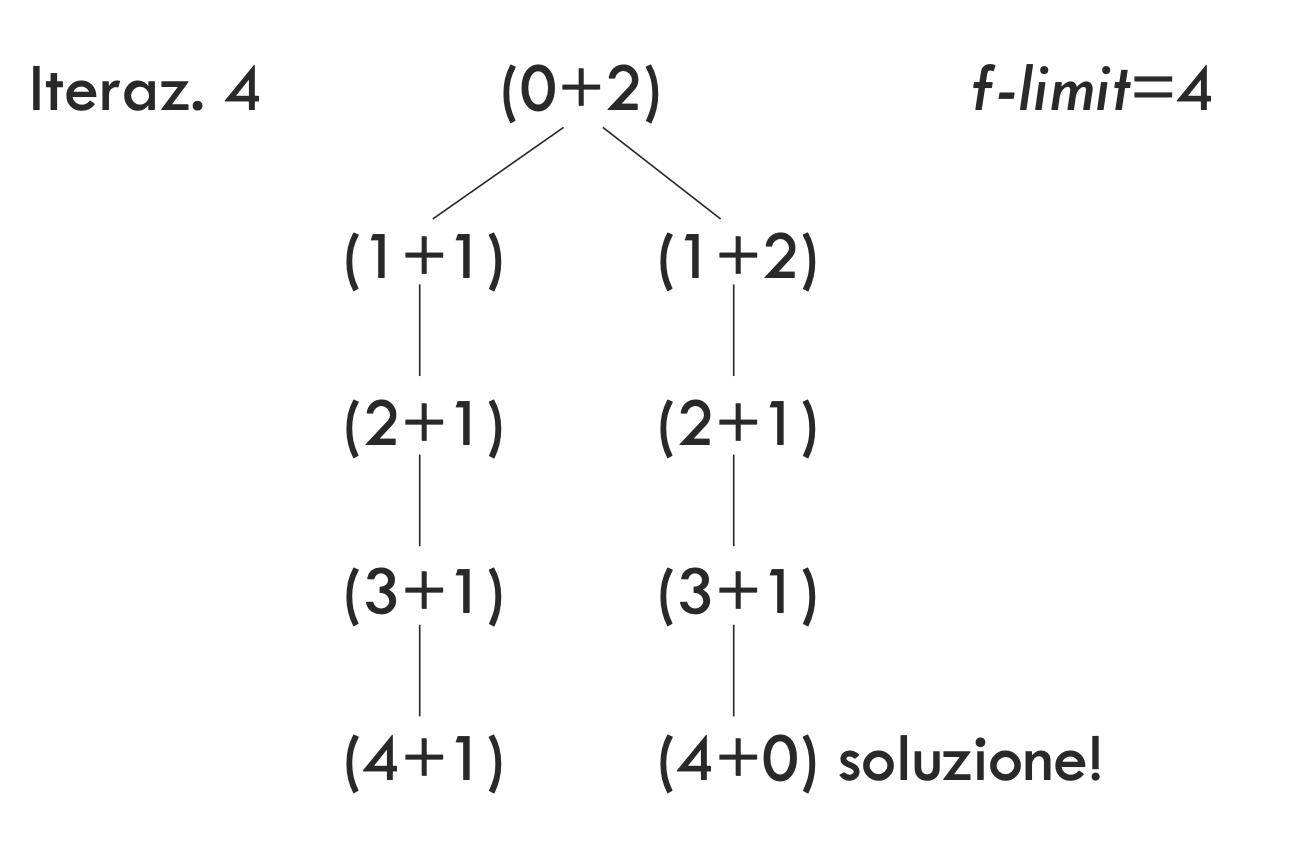
\includegraphics[width=0.65\textwidth]{images/esempio-ida*.png}
    \end{figure}
\end{example}
\hspace{-15pt}Cruciale la scelta dell'incremento per garantire l’ottimalità:
\begin{itemize}
    \item Nel caso di costo delle azioni fisso è chiaro: il limite viene incrementato del costo delle azioni.
    \item Nel caso che i costi delle azioni siano variabili? O costo minimo, oppure si potrebbe ad ogni passo fissare il limite successivo al
    valore minimo delle f scartate (in quanto superavano il limite) all’iterazione precedente.
\end{itemize}
$IDA^*$ è sia completo che ottimale.
\begin{itemize}
    \item Se le azioni hanno costo costante k (caso tipico 1) e f-limit viene incrementato di k.
    \item Se le azioni hanno costo variabile e l'incremento di f-limit è $\leq \epsilon$ (minimo costo degli archi).
    \item Se il nuovo f-limit = min. valore f dei nodi generati ed esclusi all'iterazione precedente.
\end{itemize}
L'occupazione di memoria è $O(bd)$.

\subsubsection{Best-first ricorsivo (BRFS)}
Simile a DF ricorsivo: cerca di usare meno memoria, facendo del lavoro in più. Tiene traccia ad ogni livello del \textbf{migliore percorso
alternativo}. Invece di fare backtracking in caso di fallimento (DF si ferma solo in fondo) interrompe l’esplorazione quando
trova un nodo meno promettente (secondo f). Nel tornare indietro si ricorda il miglior nodo che ha
trovato nel sottoalbero esplorato, per poterci eventualmente tornare Memoria: lineare nella profondita delle sol. ottima.
\begin{example}
    \begin{figure}[h!]
        \centering
        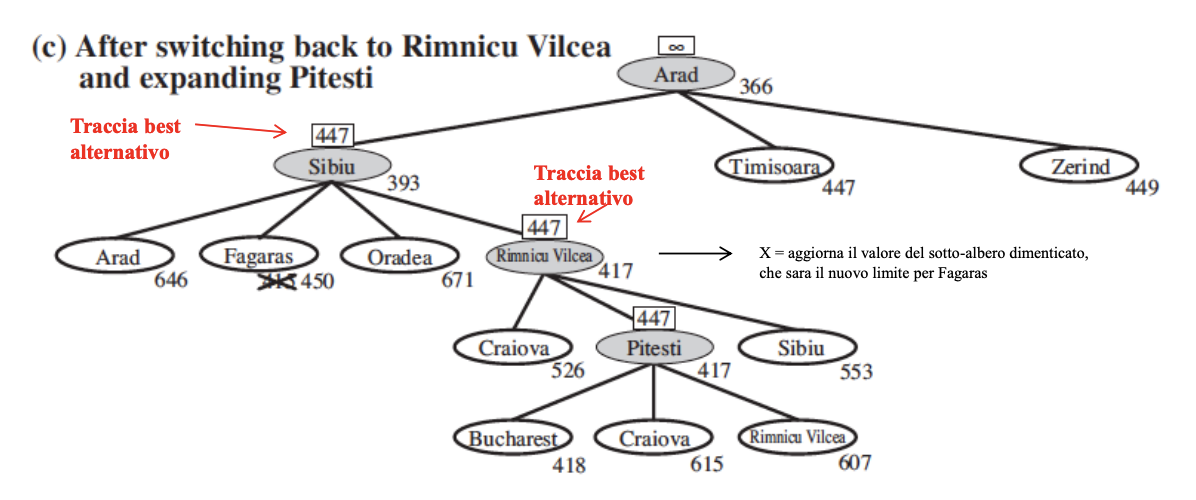
\includegraphics[width=0.65\textwidth]{images/esempio-best-first-ricorsivo.png}
    \end{figure}
\end{example}
\begin{lstlisting}
    function Ricerca-Best-First-Ricorsiva(problema)
        returns soluzione oppure fallimento
        // all inizio f-limite e un valore molto grande
        return RBFS(problema, CreaNodo(problema.Stato-iniziale), infinito) 

    function RBFS (problema, nodo, f-limite)
        // restituisce due valori
        returns soluzione oppure fallimento e un nuovo limite all f-costo 
        if problema.TestObiettivo(nodo.Stato) then return Soluzione(nodo)
        successori = [ ]

        for each azione in problema.Azioni(nodo.Stato) do
            aggiungi Nodo-Figlio(problema, nodo, azione) a successori // genera i successori
        if successori vuoto then return fallimento, infinito

        for each s in successori do // valuta i successori
            s.f = max(s.g + s.h, nodo.f) // un modo per rendere monotona f
        loop do
            migliore = il nodo con f minimo tra i successori
            if migliore.f > f_limite then return fallimento, migliore.f
            alternativa = il secondo nodo con f minimo tra i successori
            risultato, migliore.f = RBFS(problema, migliore, min(f_limite, alternativa))
            if risultato != fallimento then return risultato
\end{lstlisting}

\subsubsection{$A^*$ con memoria limitata (versione semplice)}
L'idea è quella di utilizzare al meglio la memoria disponibile. $SMA^*$ procede come $A^*$ fino ad esaurimento della
memoria disponibile. A questo punto \textbf{“dimentica” il nodo peggiore}, dopo avere aggiornato il valore del padre.
A parità di f si sceglie il nodo migliore più recente e si dimentica il nodo peggiore più vecchio. Ottimale se il cammino soluzione sta in memoria.\\\\
In conclusione in algoritmi a memoria limitata (IDA* e SMA*) le limitazioni della memoria possono portare a compiere
molto lavoro inutile [esp. ripetuta stessi nodi]. Difficile stimare la complessità temporale effettiva. Le limitazioni di memoria possono rendere un problema intrattabile dal punto di vista computazionale.
	% !TeX spellcheck = it_IT
\newpage
\section{Ricerca locale}
La ricerca \emph{euristica} nello spazio di stati è troppo costosa ed è quindi necessario utilizzare metodi diversi. \\ Se prima gli algoritmi restituivano un cammino soluzione per raggiungere un goal, ora il goal è la soluzione stessa al problema. Gli algoritmi di ricerca locale sono adatti per problemi in cui:
\begin{itemize}
	\item La sequenza di azioni non è importante ma conta solo lo stato goal
	\item Tutti gli elementi della soluzioni sono nello stato ma alcuni vincoli sono violati
\end{itemize}
Questi algoritmi non sono sistematici e tengono traccia solo del nodo corrente spostandosi su quelli adiacenti. \\
Non tengono traccia dei cammini: rendono più efficiente l'occupazione della memoria e possono trovare soluzioni anche in spazi di stati molto grandi o infiniti.\\
Sono utili per risolvere problemi di \textbf{ottimizzazione}:
\begin{itemize}
	\item Stato migliore secondo una funzione obiettivo $f$
	\item Lo stato di costo minore (non il cammino)
\end{itemize}
Data la funzione euristica del costo dell'obiettivo
\begin{center}
	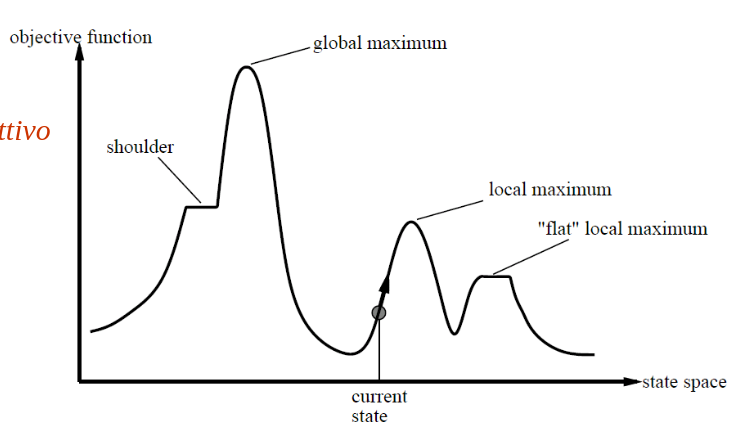
\includegraphics[scale=0.4]{ricerca_locale_spazio_stati.png}
\end{center}
uno stato ha una posizione sulla superficie e un'altezza che corrisponde al valore della valutazione della funzione obiettivo. Un algoritmo provoca movimento sulla superficie e l'obiettivo è raggiungere un punto in particolare (e.g. massimo locale).
\subsection{Hill climbing}
Sfrutta un principio di ricerca locale greedy dove vengono generati i successori e vengono valutati. Viene scelto un nodo che migliora lo stato attuale e scartati gli altri:
\begin{itemize}
	\item \textbf{Salita rapida} (o discesa): viene scelto il migliore
	\item \textbf{Stocastico}: scelta random
	\item \textbf{Prima scelta}: viene scelto il primo 
\end{itemize}
Se non ci sono successori che migliorano lo stato, l'algoritmo termina con fallimento.
\begin{lstlisting}[language=Python]
	def hill_climbing(problem):
		current = Node(problem.initial_state)
		while True:
			neighbors = [current.child_node(problem, action) for action in problem.actions(current.state)]
			if not neighbors: # se current non ha successori esci e restituisci current
				break
			# scegli il vicino con valore piu' alto (sulla funzione problem.value)
			neighbor = (sorted(neighbors,key = lambda x:problem.value(x), reverse = True))[0]
			if problem.value(neighbor) <= problem.value(current):
				break
			else:
				current = neighbor # (altrimenti, se vicino migliore, continua)
		return current
\end{lstlisting}
Non c'è frontiera a cui ritornare e si tiene un solo stato, quindi efficiente per la memoria. Il tempo necessario è variabile e dipende dal punto di partenza.\\

\subsubsection{8 regine}
Nel problema già descritto delle 8 regine, poniamo come funzione da minimizzare $h$ il numero di coppie di regine che si attaccano a vicenda. Bisogna minimizzare $h$.
Ogni regina può fare 7 mosse quindi abbiamo $7\cdot 8 = 56$ possibili stati successivi. Tra i migliori con lo stesso valore di $h$ si sceglie a caso.
\begin{example}[8 regine]
	Nel caso delle 8 regine:
	\begin{center}
		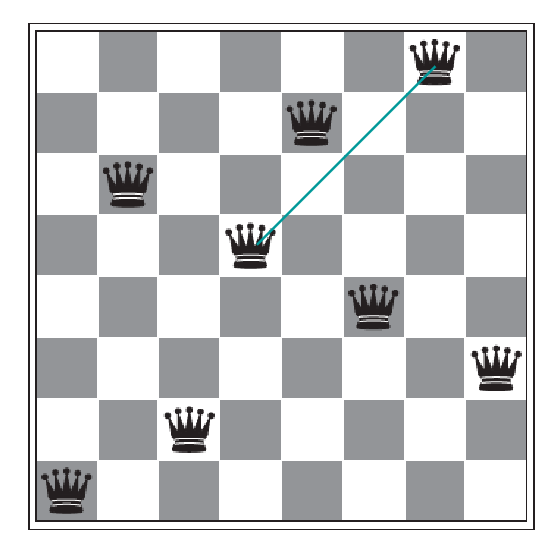
\includegraphics[scale=0.2]{8_regine_hill_climbing.png}
	\end{center}
\end{example}
Possiamo migliorare l'algoritmo in alcuni modi:
\begin{enumerate}
	\item Consentire un numero limitato di \textbf{mosse laterali}, ovvero l'algoritmo si ferma solo quando è peggiore la soluzione e non peggiore o uguale (sulle 8 regine $94\%$ di successo ma in media 21 passi)
	\item Hill-climbing \textbf{stocastico} (più lento ma soluzioni migliori)
	\item Hill-climbing \textbf{prima scelta}: genera mosse a caso fino a trovarne una migliore.
	\item Implementiamo un \textbf{riavvio casuale} che fa ripartire l'algoritmo da un punto a caso. Se la probabilità di successo è $p$, saranno necessarie $\frac{1}{p}$ iterazioni. Con molti minimi locali nella funzione obiettivo, $p$ si abbassa e aumentano il numero di volte in cui si blocca.
\end{enumerate}

\subsection{Tempra simulata}
Questo algoritmo combina hill-climbing con una scelta stocastica non totalmente casuale.\\
Ad ogni passo si sceglie un successore $n'$ a caso:
\begin{itemize}
	\item Se \textbf{migliora} lo stato corrente, viene espanso
	\item Se lo \textbf{peggiora} ($\Delta E = f(n')-f(n) \leq 0$) quel nodo viene scelto con probabilità $p=e^{\frac{\Delta E}{T}} \quad 0 \leq p \leq 1$.
\end{itemize}
Questo significa che $p$ è inversamente proporzionale al peggioramento. Con il progredire dell'algoritmo rende improbabili le mosse peggiorative.
\subsubsection{Scelta dei parametri}
I parametri sono il valore iniziale e il decremento di $T$. Il valore iniziale dovrebbe essere tale che per i valori medi di $\Delta E$ $p$ sia circa $0.5$.

\subsection{Local beam}
Dato l'algoritmo \emph{beam}, vengono salvati in memoria solo $k$ stati. Ad ogni passo si generano i successori di tutti i $k$ stati e:
\begin{itemize}
	\item Se si trova un goal, ci si ferma
	\item Altrimenti si prosegue con i $k$ migliori tra questi
\end{itemize}
\begin{note}
	È diverso da $k$ restart, in quanto non si riparte da $0$, e dal \emph{beam search} perché non si tengono tutti gli stati.
\end{note}
\subsubsection{Versione stocastica}
Si introduce un elemento di casualità: i $k$ successori vengono scelti con una probabilità maggiore per i migliori ma non tutti.
Introduciamo della terminologia:
\begin{itemize}
	\item \textbf{Organismo}: lo stato
	\item \textbf{Progenie}: i successori
	\item \textbf{Fitness}: il valore della funzione obiettivo
\end{itemize}

\subsubsection{Algoritmi genetici ed evolutivi}
Sono una variante della \emph{beam search stocastica} in cui gli stati successori sono ottenuti combinando due stati genitore invece che per evoluzione.
La \textbf{popolazione} iniziale è composta da $k$ \textbf{individui} generati casualmente e rappresentati come una stringa.
Gli individui sono valutati da una funzione di \textbf{fitness}. Vengono poi selezionati quelli per l'\textbf{accoppiamento} che danno vita alla generazione successiva in due modi:
\begin{itemize}
	\item \textbf{Crossover}: combinando il materiale genetico
	\item \textbf{Casuale}: con un meccanismo di mutazione genetica
\end{itemize}
Ogni generazione dovrebbe essere migliore della precedente.
\begin{example}[8 regine]
	Nel problema delle 8 regine abbiamo una popolazione di queste, dove le loro posizioni sono descritte da una stringa (ogni cifra è la riga in cui c'è la regina in quella colonna). La funzione di fitness è il numero di coppie di regine che non si attaccano.
	Per ogni coppia di combinazioni sulla scacchiera (scelta con la probabilità proporzionale alla fitness) viene scelto un punto di \textbf{crossing over} in maniera casuale e vengono generati due figli scambiandosi dei pezzi. Alla fine viene fatta una mutazione causale.
	\begin{center}
		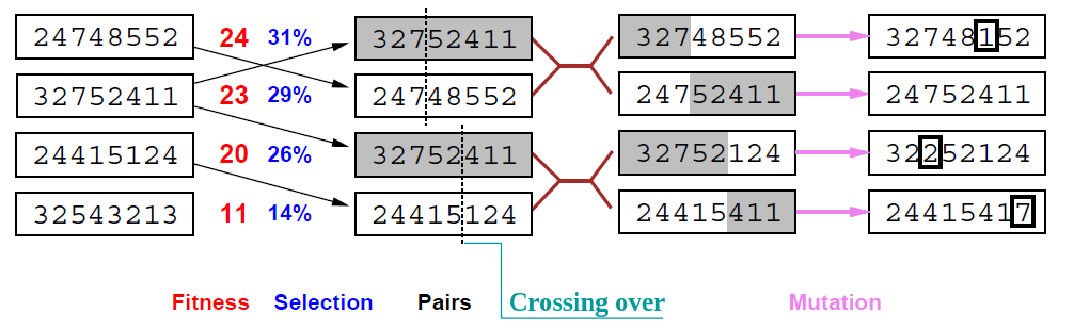
\includegraphics[scale=0.3]{alg_gen_ex.png}
	\end{center}
	\begin{center}
		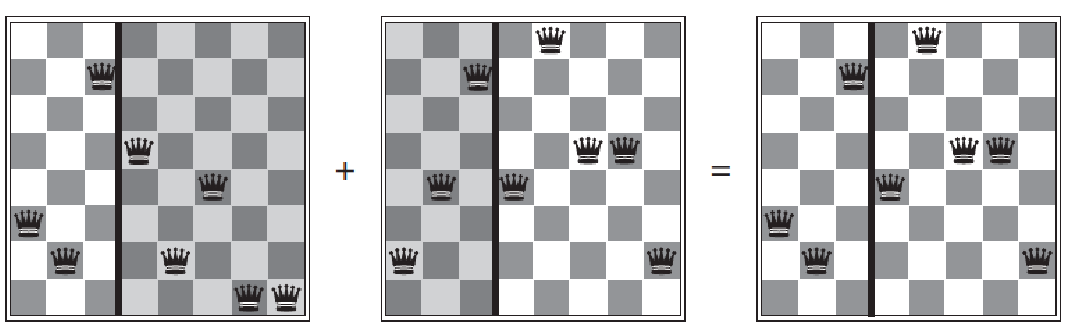
\includegraphics[scale=0.3]{alg_gen_ex_2.png}
	\end{center}
\end{example}
\noindent Questi algoritmi fanno parte del \textbf{Natural computer} e come vantaggi hanno:
\begin{itemize}
	\item Tendenza a salire della beam search stocastica
	\item Interscambio delle informazioni tra thread paralleli di ricerca in maniera indiretta
\end{itemize}
Questo tipo di algoritmi sono più efficaci se il problema ha componenti significative rappresentate in stringhe; è proprio la rappresentazione ad essere il punto critico.

\subsection{Spazi continui}
Lo stato è descritto da variabili \textbf{continue} in un vettore $x = x_1, \ldots, x_n$. Un esempio è lo spazio tridimensionale.\\
L'apparente difficoltà dovuta ai fattori di ramificazione infiniti è affrontata tramite strumenti matematici quali il \emph{gradiente}. Ad esempio l'\textbf{hill climbing iterativo} diventa:
\begin{equation*}
	x_{new} = x \pm \eta \nabla f(x)
\end{equation*}
sfruttando la direzione e lo spostamento che ci fornisce il gradiente invece di cercarlo tra gli infiniti successori.

\begin{example}
	Prendiamo la funzione $f(x)=x^2$ con derivata prima $f'(x)=2x$. Cerchiamo il minimo con
	\begin{equation*}
		x_{new}=x-\eta f'(x)
	\end{equation*}
	Partendo ad esempio da $x=2$ con $\eta=0.2$, otteniamo come primo risultato $x_{new} = 2-0.8=1.2$.
\end{example}

\subsection{Ambienti realistici}
A differenza dei problemi classici, il nostro ambiente è \textbf{parzialmente osservabile} e \textbf{non deterministico}. Qui le \textbf{percezioni} sono importanti in quanto restringono gli stati possibili e informano sull'effetto dell'azione.\\
L'agente deve elaborare una strategia con un piano di contingenza che tenga conto delle diverse eventualità.
\begin{example}[Aspirapolvere]
	\label{example:aspirapolvere}
	Un aspirapolvere imprevedibile ha due comportamenti:
	\begin{itemize}
		\item Se aspira in una stanza sporca la pulisce ma a volte pulisce anche una stanza adiacente
		\item Se aspira in una stanza pulita, a volte la sporca
	\end{itemize}
	La soluzione non è più una sequenza ma è un albero che gestisce il piano di di contingenza.
\end{example}

\subsubsection{Albero AND-OR}
È un albero che ha come nodi \emph{OR} le scelte dell'agente e come nodi \emph{AND} le diverse contingenze da considerare.
\begin{example}[Aspirapolvere]
	Nell'esempio \ref{example:aspirapolvere} l'albero sarebbe:
	\begin{center}
		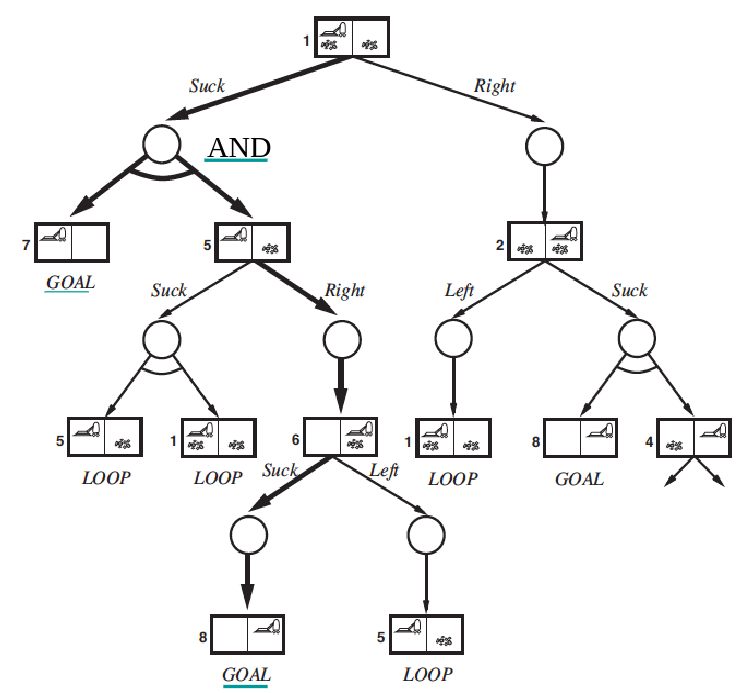
\includegraphics[scale=0.2]{example_aspirapolvere.png}
	\end{center}
\end{example}
	\newpage
\section{Agenti basati su coscenza}
Abbiamo già visto agenti con stato e con obiettivo in mondi osservabili con stati atomici e azioni descrivibili
in maniera semplice, mettendo enfasi sul processo di ricerca.\\\\
Ora andremo ad parlare di come migliorare le \textbf{capacità di ragionamento} degli agenti,
dotandoli di rappresentazioni di mondi complessi e astratti, non descrivibili semplicemente.
Agenti \textbf{basati su conoscenza}, dotati di una KB (\textbf{Knowledge Base}) con conoscenza espressa in maniera esplicita e dichiarativa.
\subsection{Introduzione}
La maggior parte dei problemi di I.A. sono “knowledge intensive”. Il mondo è tipicamente complesso: ci serve una rappresentazione
\textbf{parziale} e \textbf{incompleta} (un’astrazione) del mondo funzionale agli scopi dell’agente. Per ambienti parzialmente osservabili e complessi ci servono
linguaggi di rappresentazione della conoscenza più espressivi e capacità inferenziali. La conoscenza può essere codificata a mano ma anche estratta dai
testi o appresa dall’esperienza o estratta/elicitata dagli esperti.\\\\
La KB racchiude tutta la conoscenza necessaria a decidere l’azione da compiere in forma \textbf{dichiarativa}.
Un agente basato su conoscenza può essere costruito dicendogli (TELL) ciò che deve sapere. SI inizia con una base di conoscneza vuota
si aggiungono progressivamente formule alla base di conoscneza, una alla volta.\\\\
L’alternativa (approccio procedurale) è scrivere un programma che implementa il processo decisionale, una
volta per tutte. Un agente KB è più flessibile: più semplice acquisire conoscenza incrementalmente e modificare il
comportamento con l’esperienza.
\begin{example}
    Il mondo del Wumpus. Il mondo del Wumpus è una caverna fatta di stanze connesse tra di loro da
    passaggi. Il wumpus è una bestia puzzolente che mangia chiunque entri nella stanza in
    cui si trova. 
    \begin{figure}[h!]
        \centering
        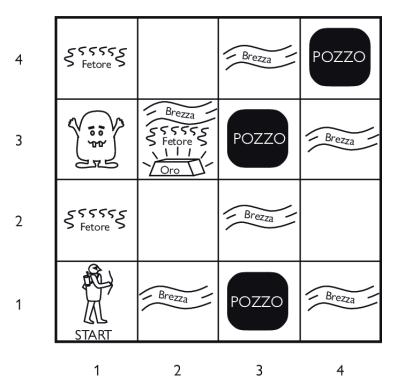
\includegraphics[width=0.4\textwidth]{images/esempio-wumpus.png}
    \end{figure}
    Il wumpus può essere ucciso dall’agente, che ha solo una freccia a disposizione.
    \begin{itemize}
        \item Ci sono stanze con dei pozzi: se l’agente entra in una di queste stanze cade nel pozzo e muore. Il Wumpus non muore nel pozzo.
        \item In una delle stanze si trova l’oro e l’obiettivo dell’agente è di trovare l’oro e tornare a casa con l’oro, sano e salvo.
        \item L’agente non conosce l’ambiente, né la sua locazione. Solo all’inizio sa dove si trova (in [1,1]).
    \end{itemize}
    Abbiamo poi delle misure di prestazioni:
    \begin{itemize}
        \item +1000 se trova l'oro, trona in [1,1] ed esce.
        \item -1000 se muore.
        \item -1 per ogni azione.
        \item -10 se usa la freccia.
    \end{itemize}
    L'\textbf{ambiente} è strutturato in una griglia 4 x 4 di stanze, circondata da pareti di delimitazione.
    L’agente comincia sempre dalla posizione [1,1], rivolto verso est (dx) ([1,1] è safe).
    Le posizioni dell’oro e del Wumpus sono scelte casualmente tra tutti I riquadri tranne quello iniziale.
    Tutti I riquadri (tranne quello iniziale) hanno una probabilita’ 0.2 di contenere un pozzo.\\\\
    Le \textbf{azioni} disponibili sono: avanti, a destra di 90°, a sinistra di 90°, afferra un oggetto, scaglia la freccia (solo una), esce.
    Le cose che vengono \textbf{percepite} (sesori) sono:
    \begin{itemize}
        \item fetore nelle caselle adiacenti al Wumpus.
        \item brezza nelle caselle adiacenti ai pozzi.
        \item Luccichio nelle caselle con l'oro.
        \item Bump se sbatte in un muto
        \item Urlo se il wumpus viene ucciso.
        \item L'agente NON percepisce la sua locaizone.
    \end{itemize}
\end{example}

\begin{figure}[h!]
    \begin{subfigure}{0.24\textwidth}
        \centering
        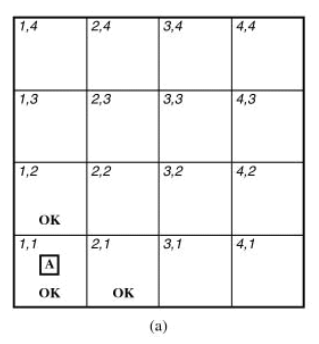
\includegraphics[width=\textwidth]{images/ess-wumpus-scenario-1.png}
        \caption{Scenario 1}
    \end{subfigure}
    \begin{subfigure}{0.24\textwidth}
        \centering
        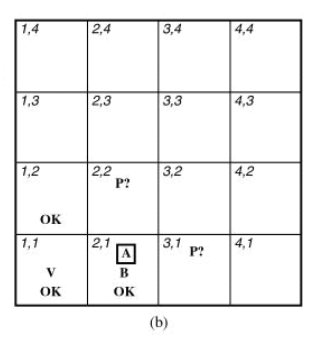
\includegraphics[width=\textwidth]{images/ess-wumpus-scenario-2.png}
        \caption{Scenario 2}
    \end{subfigure}
    \begin{subfigure}{0.24\textwidth}
        \centering
        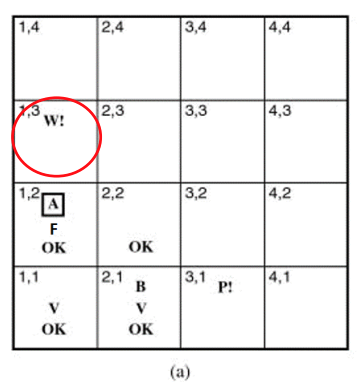
\includegraphics[width=\textwidth]{images/ess-wumpus-scenario-3.png}
        \caption{Scenario 3}
    \end{subfigure}
    \begin{subfigure}{0.24\textwidth}
        \centering
        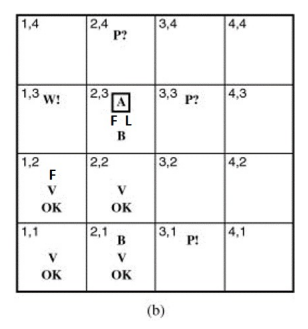
\includegraphics[width=\textwidth]{images/ess-wumpus-scenario-4.png}
        \caption{Scenario 4}
    \end{subfigure}
\end{figure}
\begin{enumerate}
    \item La percesione sono quintuple: [fetore, brezza, luccichio, bump, urlo].\\
    Percesione [1,1] = [none, none,none, none], non essendoci ne brezza ne fetore in [1,1] allora
    [1,2] e [2,1] sono sicure (OK), l'agente decide di spostarsi in [2,1].
    \item Percezione in [2,1] [none,Brezza,none,none,none].\\
    L’agente percepisce una Brezza. Quindi c’è un pozzo in [2,2] o [3,1] (P?). L’agente torna in [1,1] e poi si
    sposta in [1,2].
    \item Percezione in [1,2]: [Fetore,none,none,none,none]\\
    Il Wumpus non può essere in [1,1] (safe per definizione), né in [2,2] (altrimenti avrebbe percepito Fetore anche in [2,1]). Quindi è in [1,3].\\
    Siccome non c’è Brezza in [1,2], [2,2] è OK e ci deve essere un Pozzo in [3,1].
    \item L’agente si sposta in [2,2] e poi in [2,3]. Percezione in [2,3] [Fetore, Brezza, Luccichio, none,none].\\
    Percepisce un Luccichio, afferra l’Oro e torna sui suoi passi, percorrendo caselle OK.
\end{enumerate}

\newpage
\subsection{Agenti basati sulla conoscenza}
Un agente basato su conoscenza mantiene una \textbf{base di conoscenza} (KB): un insieme di \textbf{enunciati} (formule) espressi in un
linguaggio di rappresentazione. Interagisce con la KB mediante una interfaccia funzionale Tell-Ask:
\begin{itemize}
    \item Tell: per aggiungere nuovi enunciati a KB.
    \item Ask: per interrogare la KB.
    \item Retract: per eliminare enunciati.
\end{itemize}
Gli enunciati nella KB rappresentano le \textbf{opinioni/credenze dell’agente}. Le risposte $\alpha$ devono
essere tali che $\alpha$ \textbf{discende necessariamente} dalla KB.\\\\
Il problema: data una base di conoscenza KB, contenente una rappresentazione dei fatti che si
\textbf{ritengono veri}, come dedurre che un certo fatto a è vero di conseguenza?
$$KB |= \alpha \hspace{15pt}\text{conseguenza logica}$$
\begin{lstlisting}
    //Prende in input una percezione e restituisce un azione
    function Agente-KB (percezione) returns un azione
        //Mantiene in memoria una base di conoscenza KB che puo contenere una conoscenza iniziale.
        persistent: KB, una base di conoscenza
        t, un contatore, inizialmente a 0, che indica il tempo

        // Comunica la percezione all KB
        TELL(KB, Costruisci-Formula-Percezione(percezione, t ))

        // Chiede alla KB quale azioni deve compiere
        azione <- ASK(KB, Costruisci-Query-Azione( t ))

        // Comunica alla KB che l azione e stata compiuta al tempo t
        TELL(KB, Costruisci-Formula-Azione(azione, t ))
        t <- t + 1
        return azione
\end{lstlisting}
Base di conoscenza vs base di dati:
\begin{itemize}
    \item \textbf{base di dati}: solo fatti specifici, solo recupero (retrieval).
    \item \textbf{Base di conoscenza}: una rappresentazione esplicita, parziale e compatta, in un linguagio simbolico, che contiene:
    fatti di timpo specifico (casella [1,1] ok, c'è un posso in [3,1]), fatti di tipo generale, o regole (c'è brezza nella caselle adiacenti ai pozzi).
\end{itemize}
Qullo che caratterizza una KB è la capacità inferenziale, derivare nuovi fatti da quelli memorizzati esplicitamente (es. c'è un pozzo in [3,1] il wumpus è in [1,3]).\\
Sfortunatamente pià il linguaggio è \textbf{espressivo}, meno \textbf{efficiente} è il meccanismo inferenziale. § Il problema ‘fondamentale’ in R.C. è trovare il giusto
compromesso tra: \textbf{espressività} del linguaggio di rappresentazione, \textbf{complessità} del meccanismo inferenziale.\\
Questi due obiettivi sono in contrasto e si tratta di mediare tra queste due esisgenze.

\subsection{Logica}
Le basi di conoscenza sono costituite da enunciati (formule). Le formule sono espresse secondo le regole della sintassi,
che specifica quali di esse sono “ben formate”. La semantica di una formula esprime il “significato” della
formula. Un modello e’ una configurazione dei valori di verità che si possono assegnare alle variabili convolte in una formula.\\\\
Un formalismo per la rappresentazione della conoscneza ha tre componenti:
\begin{enumerate}
    \item Una \textbf{sintassi}: un linguaggio composto da un vocabolario e regole per la formazione delle frasi (enuciati, formule).
    \item Una \textbf{semantica}: stabilisce una corrisondenza tra gli enunciati e i fatti del mondo; se un agente ha un enunciato $\alpha$ nella KB, crede ch eil fatto corrispondente sia vero nel mondo.
    \item Un \textbf{meccanismo inferenziale} (codificato o meno tramite regole di inferenza come nella logica) che ci consente di inferire nuovi fatti.
\end{enumerate}
\begin{definition}[Semantica]
    La semantica specifica le regole usate per determinare il valore di verità di una formula nei confronti di un particolare modello.
\end{definition}
Nella logica proposizionale, un modello specifica il valore di verità (True o False) di ogni simbolo proposizionale.
\begin{figure}[h!]
    \centering
    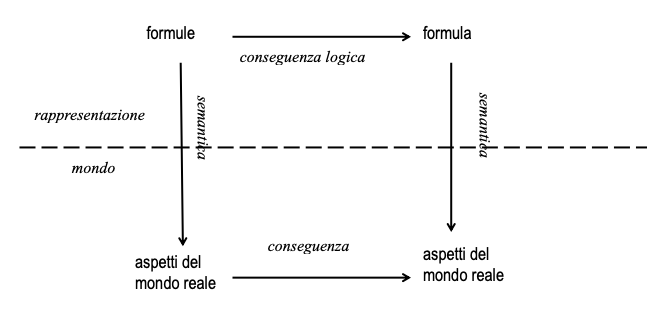
\includegraphics[width=0.65\textwidth]{images/rappresentazione_e_mondo.png}
\end{figure}

\hspace{-15pt}Le formule sono configurazioni fisiche dell’agente. 
Il ragionamento e’ il processo di costruzione di nuove configurazioni partendo dale vecchie. 
Il ragionamento logico dovrebbe assicurare che le nuove configurazioni rappresentino aspetti del mondo che sono effettive conseguenze degli aspetti delmondo rappresentati dale vecchie configurazioni
\newpage
\section{Logica Proposizionale}
\subsection{Sintassi}
\begin{definition}[Sintassi]
    La sintassi definisce quali sono le frasi leggittime (ben formate) del linguaggio.
    \begin{equation*}
        \begin{split}
            formula & \longrightarrow formulaAtomica \:\: | \:\: formula complessa \\
            formulaAtomica & \longrightarrow True \:\: | \:\: False \:\: | \:\: simbolo \\
            simbolo & \longrightarrow P \:\: | \:\: Q \:\: | \:\: R \:\:| \:\: \dots\\
            formulaComplessa & \longrightarrow \lnot formula \text{ not (negazione)}\\
            & | \:\: (formula \land formula) \text{ and (congiuzione )}\\
            & | \:\: (formula \lor formula) \text{ or (disgiunzione)}\\
            & | \:\: (formula \Rightarrow formula) \text{ implicazione}\\
            & | \:\: (formula \Leftrightarrow formula) \text{ se e solo se}\\
        \end{split}
    \end{equation*}
\end{definition}

\begin{example}
    $((A \land B) \Rightarrow C)$.
    Possiamo oettere le parentesi assumendo questa precedenza tra gli operatori:
    $$\lnot \:\: > \:\: \land \:\: > \:\: \lor \:\: > \:\: \Rightarrow, \Leftrightarrow$$
    $\lnot P \land Q \lor R \Rightarrow S$ è la stessa cosa di $(((\lnot P) \lor (Q \land R)) \Rightarrow)$. Per esempio
    dal mondo del Wumpus $P_{1,1}$ c'è il posso in $[1,1]$, $W_{2,3}$ il wumpus è in $[2,3]$.
\end{example}

\subsection{Semantica}
\begin{definition}
    La semantica specifica le regole usate per determinare il valore di verità di una formula nei confronti di un particolare modello.
\end{definition}
\hspace{-15pt}Nella logica proposizionale, un modello specifica il
valore di verità (True o False) di ogni simbolo proposizionale.\\\\
La semantica ha a che fare col significato delle frasi: definisce se un enunciato
è vero o falso rispetto a una interpretazione (mondo possibile). Una interpretazione definisce un valore di verità per tutti i simboli proposizionali.
\begin{example}
    $\{P_{1,1} \text{ vero, } P_{1,2} \text{ false, } W_{w,3} \text{ vero}\}$
\end{example}
\subsubsection{Semantica composizionale}
Il significato di una frase è determinato dal significato dei suoi componenti, a partire dalle frasi atomiche (i simboli proposizionali).
\begin{figure}[h!]
    \centering
    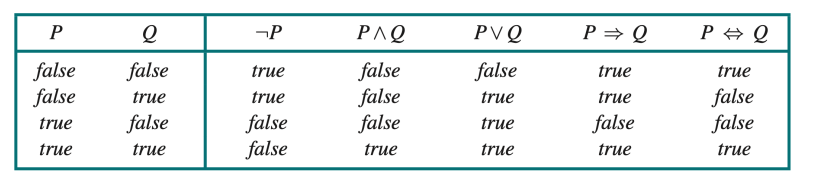
\includegraphics[width=0.65\textwidth]{images/tavola-vertià.png}
\end{figure}

\hspace{-15pt}La logica proposizionale non richiede alcuna relazione di causalità 
Per esempio per $P \Rightarrow Q$ in effetti significa che “Se P è vero, allora sostengo che lo è anche Q. Se P è falso, allora non faccio alcuna asserzione”\\\\
Una formula $\alpha$ è conseguenza logica di un insieme di
formule KB se e solo se in ogni modello di KB, anche $\alpha$
è vera ($KB \models \alpha$).\\\\
Indicando con M(KB) i modelli dell’insieme di formule
in KB e con M($\alpha$) l’insieme delle interpretazioni che
rendono $\alpha$ vera (i modelli di $\alpha$)
$$KB \models \alpha \:\: sse \:\: M(KB) \subseteq M(\alpha)$$

\subsubsection{Model checking}
Un modo (semplice) per determinare la conseguenza logica. Si enumerano i modelli. 
Si mostra che la formula $\alpha$ deve valere in tutti i modelli in cui è vera la KB.
Si usa per eseguire “inferenze logiche”, derivare una conclusione che segue logicamente da una KB
\begin{example}
    La KB iniziale $KB_0$ è costituita dalle regole generali del WW e deal fatto che la casella iniziale è safe per definizione.
    $$\lnot W_{1,1} \:\: \lnot P_{1,1} \text{ la casella iniziale è safe}$$
    Esempio di regole generate: 
    $$B_{2,1} \Leftrightarrow (P_{1,1} \lor P_{2,2} \lor P_{3,1}) \hspace{15pt} B_{1,1} \Leftrightarrow (P_{1,2} \land P_{2,1})$$
    L’agente non ha percepito nulla in [1,1] e si è spostato in [2,1] dove ha percepito una Brezza. $KB_1$ a questo punto è $KB_0$
    più i fatti corrispondenti alle percezioni $$KB_0 \cup \{\lnot B_{1,1}, B_{2,1}, \lnot F_{1,1}, \lnot F_{2,1}, \cdots\}$$
    Domandiamoci se le stanze adiacenti non contengono pozzi
    $$KB_1 \models \lnot P_{1,2} \hspace{10pt} KB_1 \models \lnot P_{2,2} \hspace{10pt} KB_1 \models \lnot P_{3,1}$$
    Cosa sappiamo all'inizio (quindi cosa c'è in $KB_0$):
    \begin{itemize}
        \item In [1,1] non ci sono pozzi: $R1: \lnot P_{1,1}$
        \item In una stanza si percepisce brezza se e solo se c’è un pozzo in una stanza adiacente (di seguito solo per le posizioni rilevanti):
        $$R2: B_{1,1} \Leftrightarrow (P_{1,2} \lor P_{2,1}) \hspace{15pt} R3: B_{2,1} \Leftrightarrow (P_{1,1} \lor P_{2,2} \lor P_{3,1})$$
    \end{itemize}
    Cosa sappiamo in base alle percezioni (cosa aggiungiamo alla KB):
    \begin{itemize}
        \item Non c'è brezza in [1,1]: $R4: \lnot B_{1,1}$
        \item C'è brezza in [2,1]: $R5: B_{2,1}$
    \end{itemize}
    \begin{figure}[h!]
        \centering
        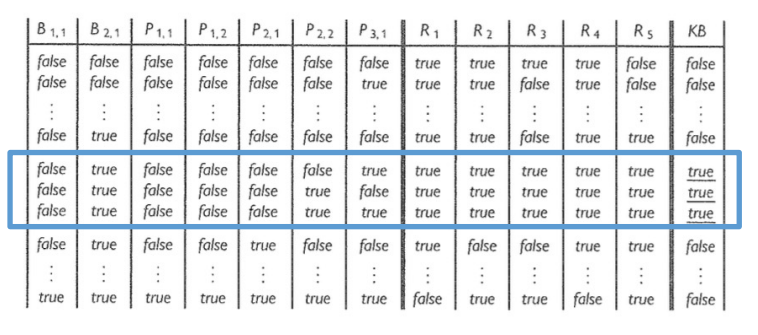
\includegraphics[width=0.5\textwidth]{images/wumpus-logica-prop.png}
    \end{figure}
    Considerando solo l’esistenza di pozzi nelle 3 caselle $P_{1,2}, P_{2,2}, P_{3,1}$ ci sono
    $2^3 = 8$ possibili interpretazioni o mondi possibili.
    \begin{figure}[h!]
        \centering
        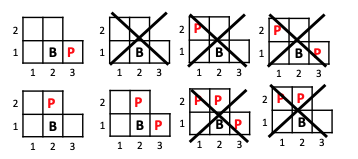
\includegraphics[width=0.5\textwidth]{images/possibili-finali-ess-wumpus-log-prop.png}
    \end{figure}
    $$KB_1 \models \lnot P_{1,2} \hspace{15pt} KB_1 \lnot P_{2,2} \lor P_{3,1} \text{ possiamo conclude che } \lnot P_{2,2} e \lnot P_{3,1} (\text{ne su }P_{2,2} \:e\: P_{3,1} \cdots)$$
\end{example}

	\newpage
\section{Calcolo proposizionale}
\subsection{Dimostrazione di teoremi}
Fin qui abbiamo visto come determinare la conseguenza logica tramite il model checking,
enumerare i modelli e mostrare che la formula deve valere in tutti. La conseguenza logica puo’ essere ottenuta anche tramite la
dimostrazione di teoremi:
\begin{itemize}
    \item applicando regole di inferenza direttamente alle formule della KB
    \item costruire una dimostrazione della formula desiderata senza consultare i modelli
\end{itemize}
Per quest'utlimo caso abbiamo tre fondamentali concetti relativi alla conseguenza logica: equivalenza logica, validià, soddisfacibilità

\subsubsection{Equivalenza logica}
Due formule $\alpha$ e $\beta$ sono \textbf{equivalenti} se sono vere nello stesso insieme di modelli.
$$\alpha \equiv \beta \Leftrightarrow \alpha \models \beta \text{ e } \beta \models \alpha$$
\begin{example}
    $A \land B \equiv B \land A \hspace{10pt} \lnot(A \land B) \equiv \lnot A \lor \lnot B \hspace{10pt} (A \land (A \lor B)) \equiv A$ 
\end{example}
\begin{figure}[h!]
    \centering
    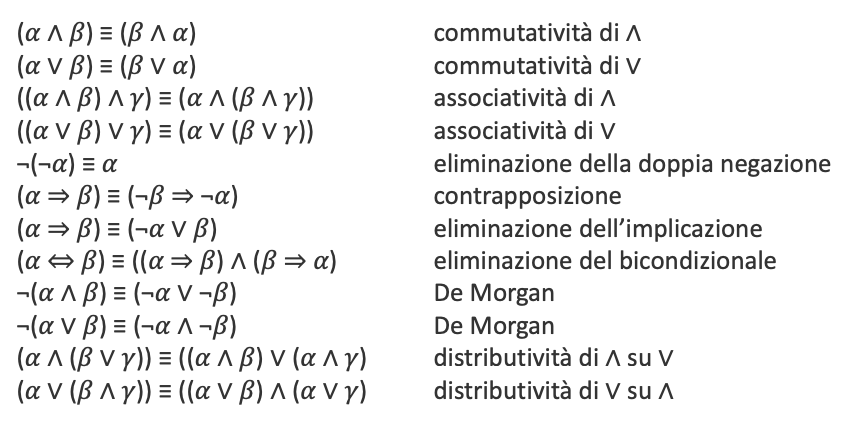
\includegraphics[width=0.65\textwidth]{images/equiv-lofiche.png}
\end{figure}

\subsubsection{Validità}
Una formula $\alpha$ \textbf{valida} sse è vera in tutte le interpretazioni.
\begin{example}
    $A \lor \lnot A$
\end{example}
\hspace{-15pt}Le formule valide sono anche dette \textbf{tautologie}, sono formule necessariamente vere.
\begin{theorem}[Teorema di deduzione]
    Date due formule $\alpha$ e $\beta$ 
    $$\alpha \models \beta \Leftrightarrow (\alpha \Rightarrow \beta) \text{ è valida}$$
\end{theorem}

\subsubsection{Soddisfacibilità}
Una formula $\alpha$ è \textbf{soddisfacibile} sse esiste una interpretazione in cui $\alpha$ è vera (ovvero se esiste un modello di $\alpha$).
\textbf{SAT}: determinare la soddisfacibilità di formule della logica proposizionale.\\\\
Validità e soddisfacibilità sono strettamente connesse:
\begin{itemize}
    \item $\alpha$ è valida sse $\lnot\alpha$ è insoddisfacibile
    \item $\alpha$ è soddisfacibile sse $\lnot\alpha$ non è valida
\end{itemize}

\subsubsection{Dimostrazione per assurdo}
Teorema di deduzione: $\alpha \models \beta$ se e solo se $(\alpha \Rightarrow \beta)$ \textbf{è valida}.\\
$\alpha \models \beta$ se e solo se $\lnot(\alpha \Rightarrow \beta)$ \textbf{è insoddisfacibile}.
Poi applico delle equivalenze logiche:
$$(\alpha \Rightarrow \beta) \equiv (\lnot\alpha \lor \beta) \text{ [eliminazione dell'implicitazione]}$$
$$\lnot(\alpha \Rightarrow \beta) \equiv \lnot (\lnot \alpha \lor \beta) \equiv (\alpha \land \lnot \beta) \text{ [De Morgan]}$$
Da questo consegue che:
$$\alpha \models \beta \Leftrightarrow (\alpha \land \lnot \beta) \text{ è insoddisfacibile}$$
Dimostrazione per refutazione o per contraddizione, si assume che $\beta$ sia falsa e si dimostra che questo porta a una contraddizione
con gli assiomi $\alpha$

\subsubsection{Inferenza per PROP}
\begin{itemize}
    \item \textbf{Model checking}: una forma di inferenza che fa riferimento alla definizione di
    conseguenza logica (si enumerano i possibili modelli), Tecnica delle tabelle di verità (TV)
    \item Algoritmi per la \textbf{soddisfacibilità (SAT)}: $KB \models \alpha \Leftrightarrow (KB \lor \lnot \alpha)$ è insoddisfacibile (\textbf{Teorema di refutazione})
    \begin{itemize}
        \item dimostrare $\alpha$ partendo da KB verificando che ($KB \land \lnot \alpha$) non è mai vero (dimostrazione per assurdo)
        \item si parte da $\lnot \alpha$ e si dimostra che questo porta a una contraddizione con gli assiomi in KB (che sono noti).
    \end{itemize}  
    La conseguenza logica può essere ricondotta a un problema SAT
\end{itemize}


	\newpage
\section{Introduzione Maching Learning}
Questo per molti è un nuovo campo, con una metodologia diversa di approccio. Infatti qui gli algoritmi non vengono usati
per risolvere un problema ma invece per creare modelli dai dati.\\
Con "Learning" (apprendimento) si intende i principi universali per gli essere viventi, la società e le macchine:\\\\
\textit{Il problema dell’apprendimento è senza dubbio al centro stesso del problema intelligenza, sia biologica che artificiale (Poggio, Shelton, AI Magazine 1999)}\\\\
Il "Learning" è quindi un obiettivo complesso, ed un campo di ricerca in continua crescita.
Il \textbf{machine learning} è emersa come un’area di ricerca che combina l'obiettivo di creare computer in grado di apprendere (IA) e nuovi potenti strumenti adattivi/statistici con basi rigorose scienza computazional.\\
Macchine che imparano da sole. Perché? Lusso o necessità?
\begin{itemize}
    \item Crescente disponibilità e necessità di analisi di dati empirici.
    \item Difficile fornire adattività/intelligenza mediante la programmazione.
\end{itemize}
Gli obbiettivi principali del ML includono:
\begin{itemize}
    \item Come metodologia AI, costruisci sistemi intelligenti adattivi (Dal motore di ricerca alla robotica).
    \item Come apprendimento statistico, costruisci un potente sistema predittivo per l'analisi intelligente dei dati (strumenti per il “data scientist”).
    \item Come metodo informatico per ambiti applicativi innovativi, usare modelli come tool per problemi complessi, interdisciplinari (dalla analisi di dati biologici per capire immagini).
\end{itemize}
Noi in particolare andiamo a studiare il ML perché è un'opportunità per conoscere \textbf{nuovi paradigmi informatici}, con un approccio diverso rispetto a alla programmazione standard, IA algoritmica/classica approcci. 
Tipico dell'area del soft computing/intelligenza computazionale. Per trovare soluzioni approssimative per problemi difficili, difficile da formalizzare
per algoritmo "fatto a mano". Costruire nuovi \textbf{sistemi intelligenti} robusti e ampiamente applicabili.
\begin{figure}[h!]
    \centering
    \includegraphics[width=0.65\textwidth]{images/ml-overview.png}
\end{figure}
\begin{example}
    Un esempio potrebbe essere riconoscere dei numeri scritti a mano.
    \begin{itemize}
        \item \textbf{Input}: abbiamo un insieme di immagini di numeri scritti a mano.
        \item \textbf{Problem}: costruire un modello che riceve come input un immagine di un numero scritto a mano e capisce che numero è.
    \end{itemize}
    La difficoltà qui sta nel \textbf{formalizzare} esattamente la soluzione del problema: infatti ci potrebbe essere
    la presenza di \textbf{"rumore"} e \textbf{ambiguità} dei dati.
\end{example}
\subsection{Apprendimento supervisionato}
Questo problema rientra nell'insieme del \textbf{Supervised learning} (classificazione, regressione).
\begin{figure}[h!]
    \centering
    \includegraphics[width=0.65\textwidth]{images/sup-learning.png}
\end{figure}
Nel apprendimento supervisionato abbiamo che:
\begin{itemize}
    \item \textbf{Given}: vengono dati degli esempi di allenamento $<input, outpu> = (x,d)$, per una funzione sconosciuta $f$.
    Il \textbf{target value} è il valore desiderato $d$ o $t$ o $y$ ... viene fornito dall'insegnamento secondo $f(x)$ per etichettare i dati.
    \item \textbf{Find}: viene trovato una buona approssimazione di $f$.
\end{itemize}
Come abbiamo già detto prima l'apprendimento supervisionato di divide in \textbf{classificazione} e \textbf{regressione}.
\begin{definition}[Classificazione]
   $f(x)$ ritorna (la presunta) classe di correttezza per $x$, $f(x)$ è funzione a valori discreti $\in \{1, 2, \dots, k\}$.   
\end{definition}
\begin{definition}[Regressione]
    Valori di uscita conitnui reali (approssimare una funzione target a valore reale, in $R, R^*$)
\end{definition}

\subsection{Apprendimento non supervisionato}
\begin{definition}[Training Set (TS)]
    Insieme di dati senza etichetta.
\end{definition}
Per esempio. Per trovare raggruppamenti naturali in un insieme di dati (clustering,
Riduzione dimensionale/Visualizzazione/Preelaborazione, modellazione della densità di dati.).
\begin{figure}[h!]
    \centering
    \includegraphics[width=0.65\textwidth]{images/unsupervides-learning.png}
\end{figure}

\subsection{Model}
Un \textbf{modello} ha l'obbiettivo di catturare/descrivere le relazioni tra i dati (sul base del compito). 
Va anche a definire la classe di funzioni che la macchina che apprende può eseguire implementare (spazio delle ipotesi)
\begin{example}
    Un insieme di funzioni $h(x, w)$ dove $w$ sono dei paramentri (astratti).
\end{example}
Altre definizioni importanti da dire sono le seguenti:
\begin{itemize}
    \item \textbf{Training example}: un esempio delle forma $(x, f(x) + noise)$ con $x$ che solitamente 
    è un vettore di caratteristiche, (d o t) $y = f(x) + noise$ è chiamato il valore target.
    \item \textbf{Target function}: la vera funzione $f$.
    \item \textbf{Ipotesi}: Una funzione proposta h ritenuta simile a f. Un espressione in un dato linguaggio che descrive le relazioni tra i dati.
    \item \textbf{Spazio di ipotesi}: Lo spazio di tutte le ipotesi (modelli specifici) che può, in linea di principio, essere prodotto dall'algoritmo di apprendimento.
\end{itemize}
Fortunatamente già conoscete alcuni linguaggi in cui esprimere relazioni che possiamo usare per esprimere modelli di ML (le ipotesi h):
\begin{itemize}
    \item \textbf{Logica} (proposizionale)
    \item \textbf{Equazioni numeriche}
    \item \textbf{Probabilità}: questo verrà reintrodotto per la rappresentazione della conoscenza incerta in AI (e quindi per esprimere modelli di ML)
\end{itemize}
Una prima vista dei differenti modi in cui verranno rappresentate le ipotesi.
\begin{itemize}
    \item \textbf{Liner models}
    \item \textbf{Symbolic rules}: (lo spazio delle ipotesi è basato sulla rappresentazione discreta); sono possibili regole diverse, ad ess:
    \begin{lstlisting}
        if(x1 = 0) and (x2 = 1) then h(x) = 1
        else h(x) = 0
    \end{lstlisting}
    \item \textbf{Probabilistic models}: una stima $p(x,y)$
\end{itemize}

\subsection{Learning algorithms}
Basandosi su dati, attività e modello, apprendimento come ricerca (euristica) attraverso lo spazio delle ipotesi H di l'ipotesi migliore.
Cioè la migliore approssimazione alla funzione target (sconosciuta). Tipicamente ricercando la h con il minimo “errore”.
\begin{example}
    Per esempio i paramentri liveri del modello sono adattati al compito da svolgere, per esempio
    migliore $w$ nei modelli lineari, migliori regole per i modelli simbolici, ecc.
\end{example}
\hspace{-15pt}$H$ potrebbe non coincidere con l'insieme di tutte le possibili funzioni e la ricerca
non può essere esaustiva: occore fare delle ipotesi, noi vedremo il ruolo del bias induttivo.
\begin{figure}[h!]
    \centering
    \includegraphics[width=0.5\textwidth]{images/learning-algo.png}
\end{figure}

\hspace{-15pt}\textbf{Apprendimento}: cercare una \textbf{buona funzione} in una funzione
spazio dai dati noti (in genere riducendo al minimo un errore/perdita).
\begin{definition}
    \textbf{Buon} w.r.t. errore di generalizzazione: misura come
    il modello prevede con precisione su nuovi campioni di dati
    (Errore/perdita misurata su nuovi dati) (errore basso, alta precisione e viceversa)
\end{definition}
\hspace{-15pt}La generalizzazione è un punto cruciale nel ML. Essa comprende:
\begin{itemize}
    \item \textbf{Fase di apprendimento}(formazione, adattamento): costruire il modello
    dai dati conosciutidati di addestramento (e bias)
    \item \textbf{Fase predittiva} (test): applicare a nuovi esempi (prendiamo gli input x’; calcoliamo la risposta secondo il modello; confrontiamo con il suo bersaglio che il modello non ha mai visto).
    Valutazione dell’ipotesi predittiva, cioè del \textbf{capacità di generalizzazione}.
    \item \textbf{Teoria}: Per esempio. Teoria dell'apprendimento statistico. In quali condizioni (matematiche) un modello è in grado di farlo generalizzare?
\end{itemize}
\begin{note}
    Le performance in ML sono uguali all'accuratezza nelle previsioni, stimato dall'errore calcolato sul set di test (Hold out).
\end{note}
	\newpage
\section{Concept learning}
Il Concept Learning per esempio è la ricerca in spazi impotetici. Lo guardiamo perché è 
un'opportunità per dare uno sguardo ad un semplice apprendimento simbolico e come base per la sucessiva
introduzione di modelli flessibili.\\\\
Un altro caso sono gli spazi discreti (rappresentazione simbolica del bersaglio funzione), sono struttura dello
spazio delle ipotesi.\\\\
Il problema dell'apprendimento prevede di imparare come migliorare con l'esperienza in qualche compito. Migliorare oltre una task T,
tenendo conto di una misura di performance P e basandosi sull'esperienza E.

\begin{definition}
    Il concept learning si definisce come inferire una funzione booleana da esempi di tringing
    positivi e negativi.
    $$c: X \to \{t,f\} \:\:or\:\: \{+, -\} \:\:or\:\: \{yes, no\} \:\:or\:\: \{0,1\}$$
    con X che è lo spazio di instanze.
\end{definition}
\hspace{-15pt}Un esempio di concepts potrebberro essere "gatto" in animale o "sport-divertente" in giorni.
\begin{figure}[h!]
    \centering
    \includegraphics[width=0.5\textwidth]{images/ess-concept-learning.png}
\end{figure}
\begin{definition}
    Si definisce "\textbf{esempio}": $<x, c(x)>$ (o $<x,d>$) in D (o nell'insieme TR).
\end{definition}
\begin{definition}
    Si dice che $h: X\to \{0,1\}$ \textbf{soddisfa} $x$ se $h(x) = 1$
\end{definition}
\begin{definition}
    Una ipotesi $h$ è \textbf{consistente}
    \begin{itemize}
        \item Con un esempio $<x, c(x)>$, con $x \in X$ se $h(x) = c(x)$
        \item Con D, se $h(x) = c(x)$ per ogni esempio di training $<x, c(x)> \in D$
    \end{itemize}
\end{definition}
\begin{figure}[h!]
    \centering
    \includegraphics[width=0.65\textwidth]{images/learning-boolean-functions.png}
\end{figure}
\hspace{-15pt}Il problema dell'\textbf{ill posed} dice che: ci sono $2^{16} = 2^{2^4} = 65536$ possibili funzioni booleane
oltre quattro funzioni booleane di input. Noi non possiamo sapere quale sia corretta finché non abbiamo visto ogni possibile coppia
input-output. Dopo 7 esempi, noi continuiamo ad avere $2^9$ possibilità.
\begin{definition}
    Nel caso generale $|H| = 2^{\#-instances} = 2^{2^n}$ per inputs/outputs binari, e con n = dimensione input.
\end{definition}
\hspace{-15pt}\textbf{Per lavorare con spazi di ipotesi ristretti}: dobbiamo iniziare scegleindo uno spazio 
di ipotesi $H$ che è considerabile più piccolo rispetto allo spazio di tutte le possibili soluzioni.

\subsection{Regole congiuntive}
Quando ci chiediamo quante possibili $h$ abbiamo, è come chiedersi quante regole congiuntive semplici nell'esempio della tabella dei valori binari.\\
Nel caso generale:
\begin{itemize}
    \item Letterali positivi, per esempio: $h_1 = l_2 \:\:\: h_2 = (l_1 \land l_2) \:\:\: h_3 = true, \dots$\\
    \textbf{Regole congiuntive semplici} $|H| = 2^n$ (immaginando $l_i$ come un bit di una stringa di lunghezza n)
    \item Letterali (anche \textbf{not}($l_i$)) \hspace{15pt} $|H| = 3^n + 1$
\end{itemize}
\begin{example}
    Esempio di training per il concept.
    \begin{itemize}
        \item \textbf{Concept}: giorni il cui l'amico Aldo si diverte con il suo sport preferito.
        \item \textbf{Task}: prevedere il valore di "Enjoy Sport" per un giorno arbitrario in base ai valori degli altri attributi attributi.
    \end{itemize}
    \begin{figure}[h!]
        \centering
        \includegraphics[width=0.5\textwidth]{images/training-esamples-concept-ler.png}
    \end{figure}
\end{example}
\subsubsection{Rappresentazione di ipotesi}
Un ipotesi $h$ è una congiunzione di vincoli sugli attributi. Ogni vincolo può contenere:
\begin{itemize}
    \item Uno specifico valore. Ess. Water=Warm
    \item Un valore che non mi interessa: Ess. Water=?
    \item Un valore non consetito (iporesi null). Ess. Water=$\O$
\end{itemize}
\begin{example}
    Un esempio di ipotesi $h$:\\
    Sky \hfill Temp \hfill Humid \hfill Wind \hfill Water \hfill Forecase\\
    Sunny \hfill ? \hfill ? \hfill Strong \hfill ? \hfill Same
    \begin{note}
        Questa è una funzione $h$, non un esempio di input.
    \end{note}
    \hspace{-15pt}Questa roba corrisponde alla funzione booleana:
    $$Sky = Sunny \land Wind = Strong \land Forecase = Same$$
    \begin{figure}[h!]
        \vspace{-15pt}
        \centering
        \includegraphics[width=0.5\textwidth]{images/rapre-ipotesi-ess.png}
    \end{figure}
\end{example}
\begin{definition}
    Task di apprendimento di concetti prototipici:
    \begin{itemize}
        \item \textbf{Given}
        \begin{itemize}
            \item \textbf{Istanza} X: Per esempio i possibili giorni descritti da degli attributi (Sky, Temp, Humidity, Wind, Water, Forecase)
            \item \textbf{Target function} c: EnjoySport X $\to \{0, 1\}$
            \item \textbf{Ipotesi H}: una congiunzione di (insieme finito di) letterali \\
            ess. $<$Sunny\:\: ? \:\:?\:\: Strong \:\:?\:\: Same $>$
            \item \textbf{Training examples} D: esempi positivi e negativi di una funzione target: $<x_1, c(x_1), \dots, <x_n, c(x_l)>$ ($l$ esempi)
        \end{itemize}
        \item \textbf{Trovare}: una ipotesi $h \in H$ tale che $h(x) = c(x)$ per ogni $x \in X$
    \end{itemize}
\end{definition}
Chiamiamo l'operazione di \textbf{Learning} la ricerca di ipotesi nello spazio $H$.\\\\
\textbf{Ipotesi dell'apprendimento induttivo}: Assumiamo in queste lezioni che "qualsiasi ipotesi trovata per approssimare la funzione target rispetto agli
esempi, andrà inoltre ad aprossimare la funzione target ben oltre gli esempi osservati".\\\\
$h=(x)$ per ogni $x \in D$ (ess. consistenza con D) \hspace{15pt} $h(x) = c(x)$ per ogni $x \in X$ \footnote{Un problema fondamentale del ML, analisi teorica ed empirica}\\\\
La rappresentazione per $H$ determina lo spazio di ricerca:
\begin{itemize}
    \item instance distinte: $3*2*2*2*2*2 = 96$
    \item Concetti distinti: $2^{96} = 2^{\#-instanze}$
    \item Ipotesi distinte sintatticamente (congiunzioni): $5*4*4*4*4*4 = 5120$ con 5 = sunny/cloudy/riny/?/$\O$ e 4=warm/cold/?/$\O$.
    \item Ipotesi distinte semanticamente: 1 + 4*3*3*3*3*3 = 973 (perché tutte le $h$ con $\O$ sono equivalenti a "false")
\end{itemize}
In generale: Dimensione elevata, addirittura infinita: strutturare lo spazio di ricerca può aiuto nella ricerca in modo più efficiente!

\subsubsection{Ordinamento da generale a specifico}
Consideriamo due ipotesi:
$$h_1 = <Sunny, ?, ?, Strong, ?, ?> \hspace{15pt} h_2 = <Sunny, ?, ?, ?, ?, ?>$$
Ed un insieme di instance coperte da $h_1$ e $h_2$.\\
$h_2$ impone meno vincoli rispetto a $h_1$ e quindi classifica più istanze x come positivo.
\begin{definition}
    Prendiamo $h_j$ e $h_k$ funzioni a valori booleani definite su X. Diciamo allora che $h_j$ è \textbf{più generale di o uguale a} $h_k$ (scritto come $h_j \geq h_k$) se e solo se
    $$\forall x \in X \: :\: [(h_k(x) = 1) \to (h_j(x) = 1)]$$
\end{definition}
\begin{example}
    Esempi binari $l_i: l_1 \geq (l_1 \land l_2),$ $l_1$ versus $l_2$, non comparabili. La relazione $\geq$ impone un 
    ordine di partizione (p.o.) sullo spazio di ipotesi $H$ che viene utilizzato da molti metodi di concept leargning. Possiamo approfittare di questo p.o. organizzare in modo efficiente la ricerca in H
\end{example}
\begin{figure}[h!]
    \centering
    \includegraphics[width=0.6\textwidth]{images/struttura-su-H.png}
\end{figure}

\subsection{Algoritmo Find-S}
Sfrutta l'ordine parziale m.g.t per cercare in modo efficiente $h$ (senza fare un enumerazione esplicita per ogni $h \in H$).
\begin{definition}
    Definiamo l'Algoritmo con i seguenti passaggi:
    \begin{enumerate}
        \item Inizializzo $h$ con l'ipotesi più specifica in H.
        \item Per ogni instanza di training $x$ \textbf{positiva}
        \begin{lstlisting}
        for each attribute a_i in h
            if a_i in h e soddisfatto da X
                non fare nulla
            else
                sostituisci a_i in h dal successivo vincolo piu generale, cioe
                soddisfatto da x [es. rimuovi da h i letterali non soddisfacenti x]
        \end{lstlisting}
        \item In output ritorna un ipotesi $h$.
    \end{enumerate}
\end{definition}
Ricerca su spazio di ipotesi fatto dall'algoritmo Find-S:
\begin{figure}[h!]
    \centering
    \includegraphics[width=0.65\textwidth]{images/ricerca-con-find-s.png}
\end{figure}

\hspace{-15pt}Alcune proprietà importnati dell'algoritmo find-S sono:
\begin{itemize}
    \item Lo spazio di ipotesi deve essere descritto da congiunzioni di attributi (forte limitazione)
    \item Find-S produttà l'iposeti più specifica fra quelle di H che sia anche coerente con gli esempi di training \textbf{positivi}.
    \item L'ipotesi di output $h$ sarà coerente con gli esempi negativi, a condizione che il terget conecpt sia contenuto in H. (perché $c \geq h$)
\end{itemize}
Mentre invece alcuni dei problemi relativi al Find-S sono i seguenti:
\begin{itemize}
    \item Non si può dire se l'apprendimento è convergente verso un concept target, nel senso
    che non è in grafo di determinare se ha trovato l'unica ipotesi coerente con gli esempi di training.
    \item Non è possibile stabilire quando i dati di training sono incosistenti, poiché ignora gli esemi di training negativo: nessuna tolleranza al rumore!
\end{itemize}
Perché preferire l’ipotesi più specifica? Cosa succede se ci sono più ipotesi massimamente specifiche?

\subsection{Algoritmo List-Then eliminate}
Per parlare di questo algoritmo bisogna prima parlare del \textbf{version spaces}. L'idea chiave è che: l'output
è un descrizione dell'insieme di tutte le $h$ consistenti con D. Possiamo fare questo senza enumerare tutti loro:
$$Consistent(h, D) := \forall <x, c(x)> \in D\:\: h(x) = c(x)$$
\begin{definition}
    Il \textbf{version space}, $VS_{H,D}$ che rispetta lo spazio di ipotesi $H$, e l'insieme di training D, 
    è un sottoinsieme delle ipotesi di H consistenti con tutti gli esempi di traning:
    $$VS_{H,D} = \{h \in H \:\:|\:\: Consistent(h, D)\}$$
\end{definition}
\hspace{-15pt}L'algoritmo ora si definisce con i seguenti punti:
\begin{enumerate}
    \item Dato un VersionSpace $\to$ una lista contenente ogni ipotesi in H.
    \item Per ogni esempio di training $<x, c(x)>$ si rimiove dal VersionSpace ogni ipotesi
    che è inconsistente con l'esempio di training, $h(x) \neq c(x)$
    \item L'output è una lista di ipotesi in VersionSpace.
\end{enumerate}
Una miglior rappresentazione per il Version space (by G e S):
\begin{figure}[h!]
    \centering
    \includegraphics[width=0.65\textwidth]{images/miglior-rapresentazione-version-space.png}
\end{figure}
\begin{definition}
    Ci sono vari modi per rappresentare il version space:
    \begin{itemize}
        \item Il \textbf{confine generale}, G, dello spazio delle versioni $VS_{H,D}$ è l'insieme di 
        membri generali massimi. (per H consistente con D).
        \item Il \textbf{confine specifico}, S, dello spazio delle versioni $VS_{H,D}$ è l'insieme di
        membri generali massimi (per H consistente con D)
        \item \textbf{Teorema}: ogni membro della spazio di versione si trova fra questi confini.
    \end{itemize}
\end{definition}
$$VS_{H,D} = \{h \in H \:|\: (\exists \: s \in S) \:\: (\exists \: g \in G) \:\:(g \geq h \geq s)\}$$
dove $x \geq y$ vuol dire che $x$ è più o uguale generale rispetto a $y$

\subsection{Algoritmo candidate elimination}
In questo algoritmo abbiamo che:
\begin{itemize}
    \item $G \to$ ipotesi massimali generali in $H$
    \item $S \to$ ipotesi massimali specifiche in $H$
\end{itemize}
For eatch esempio di training $d = <x, c(x)$.
\begin{itemize}
    \item if d è un esempio \textbf{positivo} allora rimuovi da G qualsiasi ipotesi che sia incoerente con d (def di VS).\\
    for each ipotesi $s \in S$ che non è consistente con d [\textbf{generalizzare S}]
    \begin{itemize}
        \item Rimuovere s da S.
        \item Aggiungere ad S tutti le generalizzazioni minime h di s tale che: h consistente con d ed un qualche membri di G è più generale rispetto ad h.
        \item Rimuovere da S ogni ipotesi che è più generale rispetto ad altre ipotesi in S.
    \end{itemize}
    \item if d è un esempio \textbf{negtivo} allora rimuovere da S ogni ipotesi che è inconsistente con d.\\
    for eatch ipotesi $g \in G$ che non è consistente con d [specilizzazione G]
    \begin{itemize}
        \item rimuovere g da G.
        \item Aggiungere a G tutte le specializzazioni minime h di g tali che: h sia consistente con d e cia sia qualche membro di S che è più specifico rispetto a h.
        \item Rimuovere da G ogni ipoesi che è meno generale rispetto ad altre ipotesi in G.
    \end{itemize}
\end{itemize}
\begin{example}
    Esempio dell'algoritmo Candidate Elimination.
    \begin{figure}[h!]
        \begin{subfigure}{0.45\textwidth}
            \centering
            \includegraphics[width=\textwidth]{images/es-candidate-elimination-1.png}
        \end{subfigure}
        \hspace{10pt}
        \begin{subfigure}{0.45\textwidth}
            \centering
            \includegraphics[width=\textwidth]{images/es-candidate-elimination-2.png}
        \end{subfigure}
    \end{figure}
\end{example}
La classificazione di nuovi dati si può fare nel seguente modo.
\begin{figure}[h!]
    \centering
    \includegraphics[width=0.6\textwidth]{images/classification-new-data.png}
\end{figure}

\subsection{Bias induttivo ed il suo ruolo}
Il nostro spazio di ipotesi non è capace di rappresentare un semplice concetto target di 
disgiunzione come il seguenti: $(Sky=Sunny) \lor (Sky=Cloudy)$. La candidate elimination sarebbe:
$$x_1 = <Sunny, Warm, Normal, Strong, <Cool, Change> + $$
$$x_2 = <Cloudy, Warm, Normal, Storng, Cool, Change> +$$
$S: \{<?, Warm, Normal, Strong, Cool, Change> \}$
$$x_3 = <Rainy, Warm, Normal, Strong, Cool, Change> -$$
$S: \{\}$\\\\
\textbf{Bias}: Assumiamo che lo spazio di ipotesi H contenga il concetto target c. In altre parole
che c sia descritto da con congiuzione (operatore AND) o da un letterale.

\subsubsection{Unbiased learning}
L'idea dietro al unbiased learning è la seguente: scegliere H che esprime ogni concetto che può
essere insegnato, ciò significa che H è l'insieme di tutti i possibili sottoinsiemi di X: il power set P(X).
\begin{example}
    $|H| = 96, |P(X)| = 2^{96} \sim 10^{28}$ concetti distinti.
\end{example}
\hspace{-15pt}H = disgiunzione, congiunzione, negazione. Ess. $<Sunny, Warm, Normal, ?, ?, ?> v <?, ?, ?, ?, ?, Change>$.
H contiene sicuramente il concetto target. A questo punto capiamo come generalizzare.\\\\
Che cosa sono S e G in questo caso?\\
Assumiamo esempi positivi $(x_1, x_2, x_3)$ ed esempi negativi $(x_4, x_5)$
$$S: \{(x_1 \lor x_2 \lor x_3)\} \hspace{15pt} G: \{\lnot (x_4 \lor x_5)\}$$
Gli unici esempi che sono classificati in modo non ambiguo sono gli esempi di training stessi (H può rappresentrli). In altre parole
per apprengere il concetto target si dovrebbe presentare ogni singola instanza in X come esempio di training.
\begin{proposition}
    Una \textbf{proprietà} importante è che un unbiased learner non è in grado di generalizzare
\end{proposition}
\begin{demostration}
    Ogni instanza non osservata verrà classificata positiva per precisamente metà delle ipotesi nel VS e negativa nell'altrà metà (rejecion).
    Infatti: $\forall h$ consistenti con $x_i$ (test), $\exists h'$ identico ad h eccetto per il fatto che $h'(x_i) <> h(x_i)$, $h\in VS \Rightarrow h' \in VS$ (ci sono identici in D, l'insieme TR).
\end{demostration}
\hspace{-15pt}Un entità che apprendet e che non fa ipotesi preliminari riguardo all'identità del concetto target non ha basi
razionali per classificare ogni instanza invisibile. (Restrizione, preferenza) Bias non vengono solo assunti per l'efficienza, 
essi servono anche per la generalizzazione, tuttovia, non ci dice ancora (quantifica) quale sia la soluzione migliore generalizzanta.
\begin{example}
    \textbf{Esempio trivial} (TR = Training set, TS = Test set)
    \begin{figure}[h!]
        \centering
        \includegraphics[width=0.5\textwidth]{images/trivial-esempio.png}
    \end{figure}
\end{example}
\hspace{-15pt}Problema: caratterizzare i bias per i diversi approcci di apprendimento.
\subsubsection{Bias induttivo}
Consideriamo le seguenti cose:
\begin{itemize}
    \item Un algoritmo di concept leargning L.
    \item Instance X, concetto target c.
    \item Esempi di trining $D_c = \{<x, c(x)>\}$
    \item Sia $L(x_i, D_c)$ a denotare l'assegnamento di classificazione all'instanza $x_i$ da L dopo il training con $D_c$.
\end{itemize}
\begin{definition}
    Il bias intduttivo di L è ogni insieme minimo di affermazioni \textbf{B} tali che per ogni concetto target c e corrispettivi dati di training $D_c$
    $$(\forall x_i \in X)[B \land D_c \land x_i] |- \:\: L(x_i, D_c)$$
    Dove $A |- B$ vuol dire che A implica logicamente B (segue deduttivamente da)
\end{definition}
\newpage
Sistema induttivo e \textbf{equivalente} sistema deduttivo.
\begin{figure}[h!]
    \centering
    \includegraphics[width=0.65\textwidth]{images/inductive-system.png}
\end{figure}
Visto questo, vediamo 3 apprendimento con il bias diversi:
\begin{itemize}
    \item \textbf{Rote learner} (lookup table): memorizzare esempi, classificare x se e solo se esso matcha con un precedente esempio osservabile. No bias induttivo $\to$ no generalizzazione.
    \item \textbf{Version space candidate elimination algorithm}. Bias: lo spazio di ipotesi contiene il concetto target $|H| = 973$ versus $10^{28}$
    \item \textbf{Find-S}: Bias: Lo spazio delle ipotesi contiene il concetto target e tutto il resto delle istanze sono istanze negative a meno che non sia implicato il contrario
    dalle sue altre conoscenze (viste come esempi positivi). In altre parole: abbiamo una bias linguistico dovuto all'AND sul
    letterali più il bias di ricerca dovuto alla preferenza della ipotesi più specifica.
\end{itemize}
	\newpage
\section{Modelli linari}
\subsection{Regression}
Un possibile esempio di regressione potrebbe essere un processo di stima di una funzione di valore
reale sulla base di un insieme finito di campioni rumorosi. Le conoscenze sarebbero $pairs(x, f(x) + random noise)$.\\
La task a questo punto sarebbe trovare $f$ per i dati nella seguente tabella.
\begin{figure}[h!]
    \centering
    \includegraphics[width=0.65\textwidth]{images/esempio-regresione.png}
\end{figure}
\begin{example}
    Esempio di modelli linari:
    \begin{figure}[h!]
        \centering
        \includegraphics[width=0.65\textwidth]{images/esempio-modelli-lineari.png}
    \end{figure}
\end{example}

\subsubsection{Univariate linear regression}
Il caso univariante, semplice regressione linieare: iniziamo con 1 valore di inputl, $x$ e 
1 valore di output $y$.
\begin{definition}
    Assumiamo che un modello $h_w(x)$ espresso come:
    $$out = h(x) = w_1x + w_0$$
    dove $w$ è il coefficiente a valore reale/paramentro libero (peso).
\end{definition}
Si cerca di avere un adattamento dei dati secondo una “linea retta”. Trovare $h$ (modello lineare) che 
meglio si adattano ai dati (da gli insieme di dati osservati dei valori $x$ e $y$). Assumiamo che la variabile data (y) è (linearmente) 
associata ad un'altra viarialbe (x) o più variabili, da $y = w_1x + w_0 + noise$, dove $w$ è il free par e $noise$ è
un errore misurato al target (con una distribuzione normale). Andiamo a costruire un modello (trovare il valore $w$) per predirre/stimare il prezzo ($y$) dei punti
per altri (osservabile) valori $x$ (prediction).
\begin{figure}[h!]
    \centering
    \includegraphics[width=0.55\textwidth]{images/task-model-esempio.png}
\end{figure}
Usiamo poi questi valori per \textbf{predirre/stimare} il prezzo (t) dei punti per altri valore osservabili.
\begin{figure}[h!]
    \centering
    \includegraphics[width=0.55\textwidth]{images/uso-predizione-esempio.png}
\end{figure}

\subsubsection{Learning via LMS}
Abbiamo capito che quindi dobbiamo andare a trovare i valori dei paramentri $w$ ($w_1$ e $w_2$ nei casi univarianti) per andare a minimizzare 
l'output dell'errore del modello (per eseguire un buon fitting). In uno spazio di ipotesi infinito (valore $w$ continuo) abbiamo una buona soluzione
data dalla matematica classica, possiamo "imparare" da dei semplici tools, sebbene semplice incluse moltri concetti rileventi per
il ML moderno ed è alla abse dei metodi evoluti in the field. Definiamo qui una \textbf{funzione less / error} e usiamo il \textbf{Least Mean Square (LMS)} approccio.\\\\
\textbf{Il training} si fa trovando $w$ tale che minimizzi l'\textbf{errore}/la \textbf{perdita epirica} (il miglior dato che fitta nel training set con l'esempio $l$)

\begin{definition}
    Andiamo allora a definire LMS con:
    \begin{itemize}
        \item \textbf{Given} un insieme ti esempi di training $l$ ($x_p, y_p$) $p = 1 \dots l$
        \item \textbf{Trovare} $h_w(x)$ nella forma $w_1 x + w_0$ (quindi i valori di $w$) che minimizzano la perdita attesa dei dati di training.
    \end{itemize}
    Per la perdita usiamo la radice dell'errore.\\
    Da qui il \textbf{least (mean) square} si tratta di trovare la $w$ che minimizzi la somma residua delle ragdici [$argmin_w Error(w) in L_2$]
    $$Loss(h_w) = E(w) = \sum_{p=1}^{l} (y_p - h_w(x_p))^2 = \sum_{p=1}^{l}(y_p - (w_1 x_p + w_0))^2$$
    Dove $x_p$ è $p-th$ input/pattern/esample, $y_p$ l'output per $p$, $w$ free par., $l$ numero degli esempi.
\end{definition}
\hspace{-15pt}Perché usare LMS per adattarsi ai dati con $h$? Il \underline{least (mean) square} trova $w$ per minimizzare la \textbf{somma di radici residua} [$argmin_w Error(w) \in L_2$]:
\begin{figure}[h!]
    \centering
    \includegraphics[width=0.6\textwidth]{images/lms.png}
\end{figure}

\hspace{-15pt}Il metodo dei minimi quadrati è un approccio standard alla soluzione approssimata di sistemi sovradeterminati, cioè insiemi di equazioni
in cui ci sono più equazioni che "sconociuti".\\\\
\textbf{Come si risolve?} Ricorda che il minimo locale è un punto stazionario, il gradiente è nullo.
$$\frac{\partial E(wi)}{\partial w_i} = 0 \hspace{15pt} i = 1, \dots, dim\_input + 1$$
Per una semplice regressione lineare (2 paramentri liberi) abbiamo che:
$$\frac{\partial E(w)}{\partial w_0} = 0 \hspace{15pt} \frac{\partial E(w)}{\partial w_1} = 0$$
Funzione di perdita convessa $\Rightarrow$ abbiamo la seguente soluzione (senza minimo locala).
$$w_1 = \frac{\sum x_p y_p - \frac{1}{l}\sum x_p \sum y_p}{\sum x_p^2 - \frac{1}{l} (\sum x_p^2)} = \frac{Conv[x, y]}{Var[x]}, \hspace{10pt} w_0 = \overline{y} - w_1 \overline{x} \hspace{20pt} \overline{y} = \frac{1}{l}\sum_{p \to 1} t_p  \hspace{7pt} \overline{x} = \frac{1}{l}\sum_{p\to 1}x_p$$
Calcolare il gradiante per 1 (ciascuno, omettendo quindi $p$ per $x$) pattern p. 
$$\frac{\partial E}{\partial w_i} = \frac{\partial (y - h_w(x))^2}{\partial w_i} = 2(y - h_w(x))\frac{\partial (y - h_w(h))}{\partial w_i} = 2(y - h_w(x))\frac{\partial (y - (w_1 x + w_0))}{\partial w_i}$$

\subsection{Summarizing}
\begin{itemize}
    \item \textbf{Given} un insieme di $l$ esempi di training ($x_p, y_p$) ed una funzione di perdita.
    \item \textbf{Find} il valore del peso $w$ per costruire $h_w(x)$ espresso come $y/out = w_1 x + w_0$ (minimizzare la perdita attesa dei dati di training)
\end{itemize}
\begin{figure}[h!]
    \centering
    \includegraphics[width=0.55\textwidth]{images/summarizing.png}
\end{figure}
Ora è possibile usarlo per nuovi $x'$ per predirre $y'$. Vediamo ora un approccio differente.

\subsection{Gradiant descent (ricerca locale)}
Errore delle superfici per il linear model con 2 pesi. Parabolico per $E(w) = E([w_0, w_1]^T)$ (funzione quadratica convessa)
\begin{figure}[h!]
    \centering
    \includegraphics[width=0.4\textwidth]{images/error-surface.png}
\end{figure}

\hspace{-15pt}Spazio ipotetico con 2 parametri $w_0, w_1$. Il gradiente di $E(w)$ è il nostro "compasso" per trovare il minimo.\\\\
La derivazione precedente suggerisce la linea per costruire un \textbf{algoritmo iterativo} basato su $\frac{\partial E(w)}{\partial w_i}$
\begin{definition}
    \textbf{Gradiente} = direzione salita, possiamo muoverci verso il minimo con un gradiente in discesa ($\Delta w =$ gradiente di $E(w)$)
\end{definition}
\begin{definition}
    \textbf{ricerca locale} inizia con vettore di pesi iniziali. Esso viene modificato iterativamente per diminuire
    fino a minimizzare la funzione di errore (discesa più ripida).
    $$w_new = w + \eta \cdot \Delta w$$
    Dove $\eta$ è una constante (step size) chiamata \textbf{learning rate}
\end{definition}
\begin{figure}[h!]
    \centering
    \includegraphics[width=0.5\textwidth]{images/gradieant-descent.png}
\end{figure}
Le motivazioni intuitive del gradiant descent sono che dalla formulazione, $w_new = w + \eta \cdot \Delta w$ possiamo ottenere:
$$\Delta w_0 = -\frac{\partial E(w)}{\partial w_0} = 2(y- h_w(x)) \hspace{15pt} \Delta w_1 = -\frac{\partial E(w)}{\partial w_i} = 2(y - h_w(x)) \cdot x$$
\begin{definition}
    Questa è una "error correction rule" chiamata \textbf{delta rule} che cambia la proporzione $w$ con l'errore (target-output):
    \begin{itemize}
        \item (target y - output) = err  = 0 $\to$ nessuna correzione 
        \item output > target $\to$ (y - h) < 0 (output troppo alto)
        \begin{itemize}
            \item Se $\Delta w_0$ negativo $\to$ si riduce $w_0$ e 
            \item if (input $x > 0$) $\Delta w_1$ negativo $\to$ si ricude $w_q$ else si aumenta $w_1$
        \end{itemize}
        \item output < target $\to$ $(y - h) > 0$ (output è troppo lento)
    \end{itemize} 
\end{definition}
\hspace{-15pt}In questo modo andiamo a migliorare l'apprendimento dai precedenti errori.\\\\
In conclusione possiamo dire che l'approccio del Gradiant descent è semplice ed efficacie per ricerca locale e approcci alla soluzione LMS, inoltre
ci permette di cercare in uno spazio infinito di ipotesi, può essere facilmente applicato sempre per $H$ contuno e perdite differenziabili non solo ai modelli lineari
(ess. reti neurali e deep learning models). A livello di efficienza molti miglioramenti sono possibili come il Newton's method, Conjugate Gradiant.

\subsection{Estensioni a $l$ dati}
\begin{definition}
    Possiamo riassumente per $l$ patterns $(x_p, y_p)$ nel seguente modo.
    $$\Delta w_0 = - \frac{\partial E(w)}{\partial w_0} = 2 \sum_{p=1}^{l}(y_p - h_w(x_p)) \hspace{15pt} \Delta w_1 = -\frac{\partial E(w)}{\partial w_1} = 2 \sum_{p=1}^{l}(y_p - h_w(x_p)) \cdot x_p$$
    Dove $x_p$ è un p-esmo input, $y_p$ l'output per $p$, $w$ una coppia libera, $l$ numero di esempi.
\end{definition}
\hspace{-15pt}Possiamo aggiornare $w$ dopo (ripetendo) una fase di dati di training $l$ $\to$ \textbf{algoritmo di batch} (blu). Oppure
possiamo aggiornare $w$ dopo ogni pattern $p \to$ \textbf{on-line algorithm} (discesa del gradiente stocastico) (purple and green), questo caso 
potrebbe essere più veloce, ma necessitare di step più piccoli.

\subsection{Estendere a vettori di input}
Questo è una caso standard, usare da 2 finoa centinaia di variabili/features di input  $x = [x_1, x_2, \cdots, x_n]$, il \textbf{pattern} di input
è un vettore.
\begin{example}
    Degli esempi potrebbero essere calcolare lo stato di una scacchiera in un gioco di dama per num. di pezzi bianchi/neri/re/catturati
    nel turno successivo: 6 variabili. $w$ peso che viene dalle "fetures sul tavolo".
\end{example}
\hspace{-15pt}Facciamo un piccolo riassunto della notazione per i dati. Prendiamo una $X$ matrice $l, x, n$ dove $l$ sono le righe
mentreh $n$ le colonne (feuteres, variabili, attributi), $p = 1, \cdots, l$ e $i = 1, \cdots n$. Abbiamo spesso bisogno di omettere alcuni
indici quando il contesto è chiaro, ad es:
\begin{figure}[h!]
    \centering
    \includegraphics[width=0.5\textwidth]{images/resume-data-notation.png}
\end{figure}
\begin{itemize}
    \item Ogni riga, $x$ generica (vettore in grassetto), un raw nella tabella: (input) esempio, pattern, instance, sample, ..., input vector, ...
    \item $x_i$ o $x_j$ (scalari): componenti $i$ o $j$ (dato un pattern, omettendo p).
    \item $x_p$ (o $x_i$) (vettor in grassetto) il p-esimo (o i-esimo) raw nella tabella = pattern $p$ (o i)
    \item $x_p,i$ (scalare) anche come ($x_p$): componente $i$ nel pattern $p$ (o usamo $x_p,j$ per il componente j, ecc.)
    \item Per il target sono solitamente usiamo solo $y_p$ con $p=1, \cdots l$ (lo stesso per $d$ o $t$)
\end{itemize}
Per la notazione di input multidimensionali andiamo ad assumere una colonna vettere per $x$ e $w$ (in grassetto). Numero 
del dato $l$, dimensione del vettore di input $n$, $y_p$ (targets) e $p = 1, \cdots, l$
$$w^t x + w_0 = w_0 + w_1 x_1 + w_2 x_2 + \cdots w_n x_n = w_0 + \sum_{i=1}^{n} w_i x_i$$
\begin{note}
    Notare che spesso, come prima, la notazione di trasposta $T$ in $w^T$ è omessa.
\end{note}
\hspace{-15pt}$w_0$ è l'intercetta, la soglia, il bias, l'offset.. Spesso è conveninente per includere la constante $x_0 = 1$ 
in modo che possiamo scriverlo come:
$$w^T x = x^T w (inner product) \hspace{15pt}x^T = [1, x_1, x_2, \cdots, x_n] \hspace{15pt} w^t = [w_0, w_1, w_2, \cdots, w_n]$$
\begin{note}
    Notare che $w$ è un parametro (libero) continuo "pesi".
\end{note}
\newpage
\hspace{-15pt}In una vista geometrica avremmo quello che si chiama \textbf{iperpiano}. Per 2 variabili avremmo:
$$x^T w = w^T x = w_0 + w_1 x_1 + w_2 x_2 \hspace{20pt} \text{(n dim)} w^t = [w_0, w_1, w_2, \cdots, w_n]$$
\begin{figure}[h!]
    \centering
    \includegraphics[width=0.2\textwidth]{images/hyperplane.png}
\end{figure}
Quindi possiamo definirlo come:
$$h(x_p) = x_p^T w = \sum_{i=0}^{n}x_{p,i} w_i$$
Possimao sintetizzare il caso con input di dimensione n, e l patterns nel seguenti modo:
\begin{itemize}
    \item \textbf{Given} un insieme di $l$ esempi di trainign $x_p, y_p$
    \item \textbf{Find} il peso del vettore $w$ che minimizzi la perdita attesa dei dati di training.
\end{itemize}
$$E(w) = \sum_{p=1}^{l}(y_p - x_p^T w)^2 = ||y - Xw||^2$$
Dove $x_p$ è il p-esimo input del vettore, $y_p$ è l'outpu per p, $w$ è la coppia libera, $l$ il numero
di esempi e $n$ la dimensione dell'input.

\subsection{Algoritmo iterativo di discesa del gradiante}
\begin{definition}
    Definiamo ora \textbf{l'algoritmo iterativo di discesa del gradiante}
    $$\Delta w_i = -\frac{\partial E(w)}{\partial w_i} = \sum_{p=1}^{l}(y_p - h_w(x_p)) \cdot x_{p,i} = w\sum_{p=1}^{l}(y_p - x_p^T w)x_{p,i}$$
    Abbiamo che il 2 è una costante che può essere ignorata nello sviluppo dell'algoritmo, mentre $x_{p,i}$ è il componente $i$ del pattern $p$
\end{definition}
\hspace{-15pt}Questo è una estensione vettoriale al gradiente molto semplice nel quale ogni x, ha il suo $w_i$ e il suo $\Delta w_i$ (come il singolo x prima).
Il vettore di gradianti per una dimensione n sarebbe il seguente:
$$
\Delta w = -\frac{\partial E(w)}{\partial w} = 
\begin{bmatrix}
    -\frac{\partial E(w)}{\partial w_1}\\
    -\frac{\partial E(w)}{\partial w_2}\\
    -\frac{\partial E(w)}{\partial w_i}\\
    \cdots\\
    -\frac{\partial E(w)}{\partial w_n}
\end{bmatrix}
= 
\begin{bmatrix}
    \Delta w_1\\
    \Delta w_2\\
    \Delta w_i\\
    \cdots \\
    \Delta w_n
\end{bmatrix}
$$
Possiamo lavorare in uno spazio a più luci senza la necessità di visualizzarlo. PS $w_0$ viene omesso sopra, puoi includerlo facilmente.\\\\
Per riassumenre possiamo spiegare l'algorimo in dei semplici passaggi:
\begin{enumerate}
    \item Iniziare con un vettore dei pesi $w_initial$ (piccolo), fissando un $\eta$ ($0 < \eta < 1$).
    \item Calcolare $\Delta w =$ -"gradiante di $E(w)$" = $-\frac{\partial E(w)}{\partial w}$ (o per ogni $w_j$)
    \item Calcolare $w_new = w + \eta \cdot \Delta w$ (o per ogni $w_j$) 
    \item Ritornare al 2 e ripetere finché non si converge o $E(w)$ è "sufficetemente piccolo"
\end{enumerate}
$\Delta w/l$ least mean square:
\begin{itemize}
    \item Batch versions ($\Delta w$ dopo ogni "epoch" dei dati "l")
    \item Stochatic/on-line version: aggiornare w per ogni pattern p (da $\Delta_p w = x_p (y_p - x_p^T w)$ senza aspettare la somma totale su $l$)
    \item $\eta$ = learning rate: seed/stabilty trade-off: può essere (gradualmente) decrementato a zero (garantendo convergenza, 
    evitando oscillazioni intorno al min.)
\end{itemize}
\begin{figure}[h!]
    \centering
    \includegraphics[width=0.6\textwidth]{images/learning-curve-examples.png}
\end{figure}
\begin{definition}
    Queste sono le \textbf{curve di apprendimento}: Mostrano come si verifica l'errore diminuisce attraverso il gradiente iterazioni di discesa.
\end{definition}
I vantaggi dei modelli lineari sono che se funzionano bene sono un modello fantastici: molto semplice,
tutte le informazioni dei dati sono in $w$, facili da interpretare, dati "rumorosi" sono accettati, Fenomeni lineari: un sogno per la scienza: ideale per realizzare un fenomeno “naturale”.
legge.

\subsection{Limitazioni}
Una delle limitazioni dei modelli lineari sono le tasks di regressione per problemi non lineari.
\begin{figure}[h!]
    \centering
    \includegraphics[width=0.3\textwidth]{images/regression-task-non-linear-problems.png}
\end{figure}

\hspace{-15pt}Proviamo ora a muoverci verso delle relazioni non-lineari. Notare che in $h_w(x) = w_1 x + w_0$ o $h_w(x) = w^T \cdot x$ 
come modelli statistici parametrici: "\textbf{lineare}" non si riferisce a questa linea rette, piuttosto al modo in cui
si verificano i coefficienti di regressione $w$ nell'equazione di regressione.\\\\
Possiamo quindi utilizzare anche input trasformati, come ad esempio $x, x^2, x^3, x^4, \cdots$ con una relazione \textbf{non lineare} input e outpout, 
gestiamo la macchina di learning (Least Square solution) sviluppandola nel seguente modo:
$$h_w(x) = w_0 + w_1 x + w_2 x^2 + \cdots + w_Mx^M = \sum_{j=0}^{M}w_j x^j$$
Detta \textbf{polynomial regression}.
\newpage
\begin{example}
    Facciamo un esempio non-lineare.
\end{example}
\begin{wrapfigure}[10]{r}{0.4\textwidth}
    \vspace{-25pt}
    \centering
    \includegraphics[width=0.2\textwidth]{images/esempio-non-lineare.png}
\end{wrapfigure}
Il risultato dell'adattamento di una funzione quadratica (in blu) $M=2$, passante un insieme di punti dati (in rosso). \\\\
Nei minimi quadrati lineari la dunzione non deve essere lineare in argomento (varibili di input) ma solo nei parametri ($w$) che sono
determinati per dare il best fit.

\subsection{Linear basis expansion}
Una generalizazzione (che mostriamo per la regressione) è la \textbf{LBE} o \textbf{linear basis expansion}, che definiamo come
$$h_w(x) = \sum_{k=0}^{K}w_k\phi_k(x)$$
L'argomento di input è un vettore con variabili aggiuntive, le quali sono trasformazioni di $x$ secondo una funzione $\phi$ ($\phi_k: R^n \to R$).
\begin{example}
    Alcuni eesempi sono:
    \begin{itemize}
        \item Rappresentazione polinomiale $x: \phi(x) = x_j^2$ o $\phi(x) = x_jx_i$ ...
        \item Trasformazione non lineare di un singolo input $\phi(x) = \log(x_k), \phi(x) = root(x)$, ...
        \item Trasformazione non lineare di input multipli: $\phi(x) = ||x||$
        \item Splines, ...
    \end{itemize}
\end{example}
\hspace{-15pt}Il numero di paramentri $K>n$. Il modello è lineare nei paramentri (anche in $\phi$, non in $x$): possiamo usare lo stesso
algorimo di learning di prima.

\begin{example}
    [1-dim $x$] \hspace{15pt} $\phi_j(x) = x^j$.
    $$h(x) = w_0 + w_1x + w_2x^2 + \dots + w_Mx^M = \sum_{j=0}^{M}w_jx^j$$
    1-dim regressione polinomiale ($K=M$). Per il numero di termini nel polinomio con D dim. input vedremo più avanti.\\\\
    O "qualsiasi altro" $\phi(x) = \phi([x_1, x_2, x_3])$
    $$h(x) = w_1x_1 + w_2 x_2 + w_3 \log(x_2) + w_4\log(x_3) + w_5(x_2x_3) + w_0$$
\end{example}
\hspace{-15pt}Vediamo ora le criticità (sia positive che negative) del basis expansion, per poi arrivare 
ai così detti approcci "\textbf{dizionari}".
\begin{itemize}
    \item \textbf{PROS}: È più espressivo: può modellare in modo più complicato
    relazioni (rispetto a quelle lineari).
    \item \textbf{CONS}: Con un'ampia base di funzioni, abbiamo bisogno di metodi per
    controllare la complessità del modello.
\end{itemize}
$$h_w(x) = w_0 + w_1x + w_2x^2 + \dots + w_Mx^M = \sum_{j=0}^{M}w_jx^j$$
\newpage
\begin{figure}[h!]
    \centering
    \begin{subfigure}{.3\textwidth}
        \includegraphics[width=\textwidth]{images/1st-order-polynomial.png}
        \caption{1st order polynomial}
    \end{subfigure}
    \begin{subfigure}{.3\textwidth}
        \includegraphics[width=\textwidth]{images/3st-order-polynomial.png}
        \caption{3st order polynomial}
    \end{subfigure}
    \begin{subfigure}{.3\textwidth}
        \includegraphics[width=\textwidth]{images/9st-order-polynomial.png}
        \caption{9st order polynomial}
    \end{subfigure}
\end{figure}

\hspace{-15pt}Notiamo che l'ultimo caso è molto più flessibile, ma potrebbe essere eccessivo. $E(w) = 0$ nei dati di training, diventa
un modello tropp complesso, scarsa rappresentazione della funzione vera (verde) (a causa del sovradattamento).\\\\
Capiamo dunque che il tradeoff della complessità è che:
\begin{itemize}
    \item Un modello troppo semplice: non fitta i dati in modo corretto \textbf{underfitting}
    \item Un modello troppo complesso: Altamente sensibile alle leggere perturbazioni dei dati \textbf{overfitting}
\end{itemize}
Vuoi scegliere la regolarizzazione per bilanciare i due casi attraverso il controllo della complessità del modello (intesa come flessibilità).
Considerando che la complessità non è dovuta al costo computazionale ma a misura della flessibilità del modello per adattarsi ai dati.

\subsection{Regularization}
\end{document}
